\Opensolutionfile{ans}[appendices/vastaukset]

\chapter*{Kertaus} \addcontentsline{toc}{chapter}{Kertaus}
    % Luonnolliset luvut esitellään nyt kokonaislukujen alussa.

% engl. \emph{natural numbers, counting numbers} ruots. \emph{naturliga tal}
% 
% 
% \laatikko{Luonnollisia lukuja käytetään kolmeen eri tarkoitukseen:
% 
% \begin{enumerate}
% \item Lukumäärien ilmoittamiseen (kardinaaliluvut)
% \item Järjestyksen ilmoittamiseen (ordinaaliluvut)
% \item Indeksointiin ja asioiden nimeämiseen
% \end{enumerate}
% }


% \subsection*{Tehtäviä}
% 
% \begin{tehtava}
% 
% Onko kardinaali vai ordinaali vai indeksointi?
% 
% \end{tehtava}

\section{Kokonaisluvut}

Yksinkertaisimmat käyttämämme luvut ovat lukumäärien ilmaisemiseen käytetyt $0, 1, 2, 3, \ldots$. Näitä kutsutaan \emph{luonnollisiksi luvuiksi}, ja niiden joukkoa eli kaikkia luonnollisia lukuja yhdessä merkitään symbolilla $\mathbb{N}$.
Nolla määritellään tässä luonnolliseksi luvuksi, mutta tästä ei ole yhteistä sopimusta: eräät pitävät nollaa luonnollisena lukuna ja toiset eivät.

Luonnollisille luvuille $m$ ja $n$ on määritelty yhteenlasku $m + n$, esimerkiksi $5 + 3 = 8$.

Luonnollisten lukujen $m$ ja $n$ kertolasku määritellään peräkkäisinä yhteenlaskuina
\laatikko{
\[m \cdot n = \underbrace{m + m + \ldots + m}_{n\text{ kpl}} = \underbrace{n + n + \ldots + n}_{m\text{ kpl}}.\]
}

Nollalla kertomisen ajatellaan olevan ''tyhjä yhteenlasku'' eli nolla:

\laatikko{
\[0 \cdot m = 0\]
}

Luonnollisten lukujen $m$ ja $n$ erotus määritellään yhteenlaskun avulla:
$m-n$ on luku $k$, jolle $k + n = m$. Kahden luonnollisen luvun erotus
ei kuitenkaan aina ole luonnollinen luku, esimerkkinä $3 - 5$.
Ratkaisemme ongelman määrittelemällä kullekin luonnolliselle
luvulle vastaluvun.

\laatikko{
Jokaisella luvulla $n$ on vastaluku $-n$, jolle pätee $n+(-n)=0$.
}

Luonnolliset luvut ja niiden vastaluvut muodostavat yhdessä
kokonaislukujen joukon
\[\mathbb{Z} = \{\ldots, -2, -1, 0, 1, 2, \ldots\}.\]
Kun käytämme kokonaislukuja, voidaan kahden luvun erotus määritellä
yhteenlaskun ja vastaluvun avulla yksinkertaisesti:

\laatikko{
\[m-n = m+(-n)\]
}

    Esimerkiksi luvun $2$ vastalukua merkitään $-2$, ja sille pätee $2+(-2)=0$. Vastaavasti luvun $-2$ vastaluku on sellainen luku, joka laskettuna yhteen luvun $-2$ kanssa antaa luvun $0$. Tämä on tietysti $2$, koska $-2+2=0$. Näin voidaan huomata, että $-(-2)=2$.
    


\subsection*{Yhteen- ja vähennyslasku}

    Kysymys: Mitä saadaan, kun luvusta $5$ vähennetään luku $-8$?
    
    Negatiivisten ja positiivisten lukujen yhteen- ja vähennyslaskut voidaan helposti tulkita lukusuoran avulla.
    
    % tässä on vähän kyseenalaista käyttää sekaisin sanallista ja numeerista esitystä
    
    $5+8$ ''viiteen lisätään kahdeksan''
    \begin{center}
      \begin{lukusuora}{-1}{14}{14}
        %\lukusuoranuolialas{5}{13}
        %\lukusuoranuolialas{0}{8}
        {\color{red} \lukusuoravaliss{0}{5}{$0$}{$5$}}
        \lukusuorauusi
        {\color{red} \lukusuoravaliss{8}{13}{$8$}{${\color{black}13}$}}
        {\color{blue} \lukusuoravaliss{0}{8}{$0$}{$8$}}
       \end{lukusuora}
       ${\color{red}5}+{\color{blue}8}=13$
    \end{center}
    
    $5+(+8)$ ''viiteen lisätään plus kahdeksan''
    
    $+8$ tarkoittaa samaa kuin $8$. '$+$'-merkkiä käytetään luvun edessä silloin, kun halutaan korostaa, että kyseessä on nimenomaan positiivinen luku.
    
%säädetään kuva vähän irti tuosta edeltävästä tektistä
%\vspace{0.3cm}     
    
    \begin{center}
          \begin{lukusuora}{-1}{14}{14}
        {\color{red} \lukusuoravaliss{0}{5}{$0$}{$5$}}
        \lukusuorauusi
        {\color{red} \lukusuoravaliss{8}{13}{$8$}{${\color{black}13}$}}
        {\color{blue} \lukusuoravaliss{0}{8}{$0$}{$8$}}
       \end{lukusuora}
       ${\color{red}5}+({\color{blue}+8})=13$
    \end{center}
    
    $5-(+8)$ ''viidestä vähennetään $+8$''
    
    Tämä tarkoittaa samaa kuin $5-8$. Lukusuoralla siis liikutaan 8 pykälää taaksepäin.

%säädetään kuva vähän irti tuosta edeltävästä tektistä
\vspace{0.3cm}     
    
    \begin{center}
              \begin{lukusuora}{-4}{8}{14}
        {\color{blue} \lukusuoravaliss{-3}{5}{\color{black}$-3$}{$5$}}
        \lukusuorauusi
%        {\color{red} \lukusuoravaliss{8}{13}{$8$}{${\color{black}13}$}}
        {\color{red} \lukusuoravaliss{0}{5}{$0$}{$5$}}
       \end{lukusuora}
       ${\color{red}5}-({\color{blue}+8})=-3$
    \end{center}


%lukiolaiset pitivät näitä epäselvinä kuvina
    
    Mitä tapahtuu, kun lisätään negatiivinen luku? Kun lukuun lisätään $1$, se kasvaa yhdellä. Kun lukuun lisätään $0$, se ei kasva lainkaan. Kun lukuun lisätään negatiivinen luku, esimerkiksi $-1$, on luonnollista ajatella, että se pienenee. Tällä logiikalla negatiivisen luvun lisäämisen pitäisi siis pienentää alkuperäistä lukua. Siksi on sovittu, että $5+(-8)$ on yhtä suuri kuin $5-8$.
    
%säädetään kuva vähän irti tuosta edeltävästä tektistä
\vspace{0.3cm}     

    \begin{center}
                 \begin{lukusuora}{-4}{8}{14}
        {\color{blue} \lukusuoravaliss{-3}{5}{\color{black}$-3$}{$5$}}
        \lukusuorauusi
%        {\color{red} \lukusuoravaliss{8}{13}{$8$}{${\color{black}13}$}}
        {\color{red} \lukusuoravaliss{0}{5}{$0$}{$5$}}
       \end{lukusuora}
       ${\color{red}5}+({\color{blue}-8})=-3$
    \end{center}
    
    
    $5-(-8)$ ''viidestä vähennetään miinus kahdeksan''
    
    Negatiivisen luvun lisääminen on vastakohta positiivisen luvun lisäämiselle. Tällöin on luonnollista, että negatiivisen luvun vähentäminen on vastakohta positiivisen luvun vähentämiselle. Koska positiivisen luvun vähentäminen pienentää lukua, pitäisi negatiivisen luvun vähentämisen kasvattaa lukua. Tämän vuoksi on sovittu, että $5-(-8)$ tarkoittaa samaa kuin $5+8$.
    
%säädetään kuva vähän irti tuosta edeltävästä tektistä
\vspace{0.3cm}     
        
    \begin{center}
    \begin{lukusuora}{-1}{14}{14}
        {\color{red} \lukusuoravaliss{0}{5}{$0$}{$5$}}
        \lukusuorauusi
        {\color{red} \lukusuoravaliss{8}{13}{$8$}{${\color{black}13}$}}
        {\color{blue} \lukusuoravaliss{0}{8}{$0$}{$8$}}
       \end{lukusuora}
       ${\color{red}5}-({\color{blue}-8})=13$
    \end{center}


\laatikko{
Yhteen- ja vähennyslaskun merkkisäännöt

\begin{itemize}
\item $a+(-b)=a-b=a-(+b)$
\item $-(-a)=a$
\item $a-(-b)=a+b=a+(+b)$
\end{itemize}
}

\laatikko{
Yhteen- ja vähennyslasku kumoavat toisensa

\begin{itemize}
\item $a+b-b=a$
\item $a-b+b=a$
\end{itemize}
}


\subsection*{Kertolasku}

    Samaan logiikkaan perustuen on sovittu myös merkkisäännöt positiivisten ja negatiivisten lukujen kertolaskuissa. Kun negatiivinen ja positiivinen luku kerrotaan keskenään, saadaan negatiivinen luku, mutta kun kaksi negatiivista lukua kerrotaan keskenään, saadaan positiivinen luku.

    $3 \cdot 4$ ''kolme kappaletta nelosia''
    
   \begin{center}
    \begin{lukusuora}{-1}{14}{14}
	\color{red} \lukusuoravaliss{0}{4}{$0$}{$4$}
	\color{red} \lukusuoravaliss{4}{8}{$4$}{$8$}
	\color{red} \lukusuoravaliss{8}{12}{$8$}{$12$}

      \end{lukusuora}
      $3\cdot {\color{red}4}=12$
    \end{center}
    
    $3 \cdot (-4)$ ''kolme kappaletta miinus-nelosia''
    
    
    \begin{center}
    \begin{lukusuora}{-13}{2}{14}
	\color{red} \lukusuoravaliss{-12}{-8}{$-12$}{$-8$}
	\color{red} \lukusuoravaliss{-8}{-4}{$-8$}{$-4$}
	\color{red} \lukusuoravaliss{-4}{0}{$-4$}{$0$}

      \end{lukusuora}
      $3\cdot ({\color{red}-4})=-12$
    \end{center}
    
    $-3 \cdot 4$ ''miinus-kolme nelinkertaistetaan''
    
    \begin{center}
    \begin{lukusuora}{-13}{2}{14}
	\color{red} \lukusuoravaliss{-12}{-9}{$-12$}{$-9$}
	\color{red} \lukusuoravaliss{-9}{-6}{$-9$}{$-6$}
	\color{red} \lukusuoravaliss{-6}{-3}{$-6$}{$-3$}
	\color{red} \lukusuoravaliss{-3}{0}{$-3$}{$0$}

      \end{lukusuora}
      ${\color{red}-3}\cdot 4=-12$
    \end{center}
    
    $-3 \cdot (-4)$ ''miinus-kolme miinus-nelinkertaistetaan''
    
    \begin{center}
    \begin{lukusuora}{-1}{14}{14}
	\color{red} \lukusuoravaliss{12}{9}{$12$}{$9$}
	\color{red} \lukusuoravaliss{9}{6}{$9$}{$6$}
	\color{red} \lukusuoravaliss{6}{3}{$6$}{$3$}
	\color{red} \lukusuoravaliss{3}{0}{$3$}{$0$}

      \end{lukusuora}
      ${\color{red}-3}\cdot (-4)=12$
    \end{center}

\subsection*{Jakolasku}

        Kun ensin kerrotaan jollain ja sitten jaetaan samalla luvulla, päädytään takaisin samaan, mistä lähdettiin.  Jakolaskujen merkkisäännöt on sovittu niin, että tämä ominaisuus säilyy. Ne ovat siis samat kuin kertolaskujen merkkisäännöt.
    
    Esimerkiksi haluamme, että $(-12):(-3)\cdot (-3)=-12$. Nyt voimme kysyä, mitä laskun $(-12):(-3)$ tulokseksi pitäisi tulla, jotta jakolasku ja kertolasku säilyvät toisilleen käänteisinä, eli mikä luku kerrottuna $-3$:lla on $-12$. Kertolaskun merkkisäännöistä nähdään helposti, että tämän luvun täytyy olla $+4$ eli $4$. Niinpä on sovittu, että $(-12):(-3)=12:3=4$.

\laatikko{
Kerto- ja jakolaskun merkkisäännöt
\begin{itemize}
\item $a\cdot (-b)=(-a)\cdot b=-(ab)$
\item $(-a)\cdot (-b)=a\cdot b=ab$
\item $(-a):b=a:(-b)=-\dfrac{a}{b}$
\item $(-a):(-b)=a: b=\dfrac{a}{b}$
\end{itemize}
}

\laatikko{
Kerto- ja jakolasku kumoavat toisensa
\begin{itemize}
\item $a\cdot b:b=a$
\item $a:b\cdot b=a$
\end{itemize}
}

    \subsection*{Jaollisuus ja tekijöihinjako}

   
    \laatikko{
    Kokonaisluku $a$ on jaollinen kokonaisluvulla $b$, jos on olemassa kokonaisluku $c$ niin, että $a = b \cdot c$. Tällöin sanotaan myös, että $b$ on $a$:n tekijä.
    }
    
    \begin{esimerkki}
    \begin{enumerate}[a)]
    \item Luku $-12$ on jaollinen luvulla $3$:lla, sillä $-12 = 3 \cdot (-4)$.
    \item $-12$ ei ole jaollinen $5$:llä, sillä ei ole kokonaislukua, joka kerrottuna viidellä olisi $12$.
    \end{enumerate}
    \end{esimerkki}
    
    

    
    Yllä jaollisuus määritellään kertolaskun avulla. Jaollisuuden voi määritellä myös jakolaskun avulla niin, että $a$ on jaollinen $b$:llä, mikäli $a:b$ on kokonaisluku. Esimerkiksi $12$ on jaollinen $3$:lla, koska $12:3 = 4$, joka on kokonaisluku.
    %Tämä määritelmä vaatii kuitenkin, että $b \neq 0$, joten sitä ei voida pitää yleispätevänä määritelmänä jaollisuudelle. Se on kuitenkin monesti yksinkertaisempi tapa ajatella.
   
    \begin{center}
     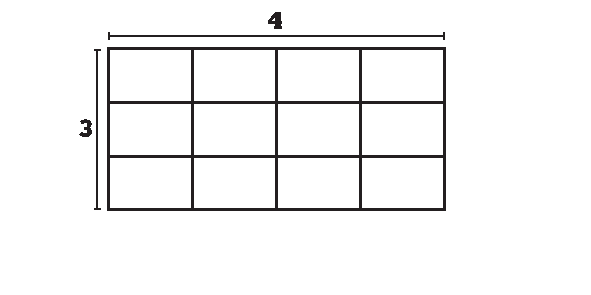
\includegraphics[scale=0.85]{pictures/Kuva2-4-3x4.pdf}
    \end{center}
    
    Kaikki luvut ovat jaollisia itsellään ja luvulla $1$. Esimerkiksi $7=7 \cdot 1=1 \cdot 7$, joten $7$ on jaollinen $1$:llä ja $7$:llä.
    
    \laatikko{
    \emph{Alkuluku} on ykköstä suurempi luku, joka on jaollinen ainoastaan luvulla $1$ ja itsellään.
    }
    
    Esimerkiksi luvut 2, 3, 5, 7, 11, 13, 17 ja 19 ovat alkulukuja.
    
    Kokonaisluvun $n$ tekijöitä, jotka ovat alkulukuja, kutsutaan alkutekijöiksi.
    
    \laatikko{
    \textbf{Aritmetiikan peruslause}
    
    Jokainen ykköstä suurempi kokonaisluku voidaan esittää yksikäsitteisesti alkulukujen tulona.
    }
    
   Aritmetiikan peruslause todistetaan kurssilla Logiikka ja lukuteoria.
    
    Esimerkiksi luku $84$ voidaan kirjoittaa muodossa $2\cdot 2\cdot 3\cdot 7$. Kokeilemalla havaitaan, että 2, 3, ja 7 ovat kaikki alkulukuja. Aritmetiikan peruslauseen nojalla tiedetään, että tämä on ainoa tapa kirjoittaa $84$ alkulukujen tulona -- mahdollista kerrottavien termien järjestyksen vaihtoa lukuunottamatta.
    
    %Kun luku $84$ esitetään muodossa $2\cdot 2\cdot 3\cdot 7$ on tapana sanoa, että se on \emph{jaettu alkutekijöihin}. Alkutekjät esitetään yleensä kasvavassa numerojärjestyksessä. Jos sama luku esiintyy tekijöissä useampaan kertaan, on se yleensä yleensä tapana merkitä potenssina. Tällöin luku $84$ voitaisiin kirjoittaa tekijöihin jaettuna $2^2\cdot 3\cdot 7$ ja luku $96$ muodossa $2\cdot 2\cdot 2\cdot 2\cdot 2\cdot 3=2^5\cdot 3$.
    
    %Luvun alkutekijät voi löytää etsimällä luvulle ensin jonkin esityksen kahden luvun tulona. Näiden kahden luvun ei tarvitse olla alkulukuja. Sen jälkeen sama toistetaan näille kahdelle luvulle ja edelleen aina uusille luvuille, kunnes tulossa on jäljellä vain alkulukuja.
    
    %\begin{esimerkki}
    %Luvun $96$ alkutekijät voi löytää vaikkapa seuraavanlaisella ketjulla: $96 = 2 \cdot 48 = 2 \cdot (2 \cdot 24) = 2 \cdot 2 \cdot (6 \cdot 4) = 2 \cdot 2 \cdot (2 \cdot 3) \cdot (2 \cdot 2)$. Nyt jäljellä on vain alkulukuja ja saatu tulo voidaan kirjoittaa lyhennettynä $96 = 2^5 \cdot 3$.
    %\end{esimerkki}


\subsection*{Lausekkeiden sieventäminen}

Matemaattisia ongelmia ratkaistaessa kannattaa usein etsiä vaihtoehtoisia tapoja jonkin laskutoimituksen, lausekkeen tai luvun ilmaisemiseksi. Tällöin usein korvataan esimerkiksi jokin laskutoimitus toisella laskutoimituksella, josta tulee sama tulos. Näin lauseke saadaan sellaiseen muotoon, jonka avulla ratkaisussa päästään eteenpäin. Kun merkitsemme monimutkaisen lausekkeen lyhyemmin, sitä kutsutaan \emph{sieventämiseksi}. Sieventäminen on ikään kuin sotkuisen kaavan siistimistä selkeämmäksi.

Matematiikassa on tapana ajatella niin, että saman luvun voi kirjoittaa monella eri tavalla. Esimerkiksi merkinnät \begin{align*}
                & 42 \\ & -(-42) \\ & 6 \cdot 7 \\ & (50-29) \cdot 2                                                                                                      
                                                                                                                 \end{align*}
tarkoittavat kaikki samaa lukua. Niinpä missä tahansa lausekkeessa voi luvun $42$ paikalle kirjoittaa merkinnän $(50-29)\cdot 2$, sillä ne tarkoittavat samaa lukua. Tähän lukuun on koottu sääntöjä, joiden avulla laskutoimituksia voi vaihtaa niin, että lopputulos ei muutu.

\laatikko{
Yhteenlaskut voi laskea missä järjestyksessä tahansa

\begin{tabular}{ll}
  $a+b=b+a$\qquad\qquad&(vaihdantalaki)\\
  \\
  $a+(b+c)=(a+b)+c=a+b+c$\qquad\qquad&(liitäntälaki)
\end{tabular} 
}

Esimerkiksi laskemalla voidaan tarkistaa, että $5+7=7+5$ ja että $(2+3)+5=2+(3+5)$.

Nämä säännöt voidaan yhdistää yleiseksi säännöksi, jonka mukaan yhteenlaskun sisällä laskujärjestystä voi vaihtaa miten tahansa.

Tämä sääntö voidaan yleistää koskemaan myös vähennyslaskua, kun muistetaan, että vähennyslasku tarkoittaa oikeastaan vastaluvun lisäämistä. $5-8$ tarkoittaa siis samaa kuin $5+(-8)$, joka voidaan nyt kirjoittaa yhteenlaskun vaihdantalain perusteella muotoon $(-8)+5$ eli $-8+5$ ilman, että laskun lopputulos muuttuu. Tästä seuraa seuraava sääntö:

\laatikko{
Pelkästään yhteen- ja vähennyslaskua sisältävässä lausekkeessa laskujärjestystä voi vaihtaa vapaasti, kun ajattelee miinusmerkin kuuluvan sitä seuraavaan lukuun ja liikkuvan sen mukana.
}

\begin{esimerkki} 
$5-8+7-2=5+(-8)+7+(-2)=(-2)+(-8)+5+7=-2-8+5+7$ 
\end{esimerkki}

Vastaavat säännöt pätevät kerto- ja jakolaskulle samoista syistä.

\laatikko{
Kertolaskut voi laskea missä järjestyksessä tahansa

\begin{tabular}{ll}
  $a\cdot b=b\cdot a$\qquad\qquad&(vaihdantalaki)\\
  \\
  $a\cdot (b\cdot c)=(a\cdot b)\cdot c=a\cdot b\cdot c$\qquad\qquad&(liitäntälaki)
\end{tabular} 
}



\begin{esimerkki}

$5 \cdot 6 = 6 \cdot 5$
 
 $2 \cdot (1+2) = 2 \cdot 1 + 2 \cdot 2$
\end{esimerkki} 

%$2 \cdot (1+2) = 2 \cdot 1 + 2 \cdot 2$

\laatikko{
Pelkästään kerto- ja jakolaskua sisältävässä lausekkeessa laskujärjestystä voi vaihtaa vapaasti, kun ajattelee jakolaskun käänteisluvulla kertomisena.
}

\begin{esimerkki}
$5:8\cdot 7:2=5\cdot\frac18\cdot 7\cdot\frac12=7\cdot \frac12\cdot\frac18\cdot 5=7:2:8\cdot 5$
\end{esimerkki} 

Lisäksi yhteen- ja kertolaskua sisältävällä lausekkeelle pätee seuraava erittäin tärkeä sääntö:

\laatikko{
$a(b+c)=ab+ac$\qquad\qquad(osittelulaki)

Vasemmalta oikealle luettaessa puhutaan sulkujen avaamisesta. Oikealta vasemmalle päin mentäessä puhutaan \emph{yhteisen tekijän ottamisesta}.
}

Aikaisemmin mainittujen laskulakien perusteella osittelulaki voidaan yhdistää koskemaan myös toisin päin olevaa kertolaskun ja yhteenlaskun yhdistelmää, useamman luvun yhteenlaskua, vähennyslaskua ja jakolaskua:

\laatikko{
\begin{itemize}
\item $(b+c)a = a(b+c) = ab+ac = ba+ca$ (Sovellettu vaihdantalakia)
\item $a(b+c+d) = a((b+c)+d) = a(b+c)+ad = ab+ac+ad$ (Sovellettu liitäntälakia)
\item $a(b-c) = a(b+(-c))=ab+a\cdot(-c)=ab-ac$ (Sovellettu vähennyslaskun määritelmää vastaluvun avulla)
\item $(b+c):a = (b+c)\cdot\dfrac1a = b\cdot\dfrac1a+c\cdot\dfrac1a = b:a+c:a$ (Sovellettu jakolaskun ilmaisemista käänteisluvun avulla. Tämä ominaisuus esitellään myöhemmin rationaalilukujen yhteydessä.)
\end{itemize}
}

Esimerkiksi seuraava laskutoimitus on helppo laskea osittelulain avulla: 
     \begin{align*}
	  2574\cdot 542-2574\cdot 541 &= 2574\cdot (542-541)  \\ &= 2574\cdot 1 \\ &= 2574
     \end{align*}


Osittelulakia voidaan käyttää myös tuntemattomia lukuja sisältävien lausekkeiden muokkaamisessa. Esim. $2(x+5)=2x+10$.
    

\subsection*{Tehtäviä}
   
    
        \begin{tehtava}
        Kirjoita laskutoimitukseksi. (Laskuun ei tarvitse merkitä yksikköjä, eli celsiusasteita tai euroja.)


        \begin{enumerate}[a)]
            \item Pakkasta on aluksi $-10~^{\circ}$C, ja sitten se lisääntyy kahdella pakkasasteella.
            \item Pakkasta on aluksi $-20~^{\circ}$C, ja sitten se hellittää (vähentyy) kolme (pakkas)astetta.
            \item Lämpötila on aluksi $17~^{\circ}$C, ja sitten se vähentyy viisi astetta.
            \item Lämpötila on aluksi $5~^{\circ}$C, ja sitten se kasvaa kuusi astetta.
            \item Mies on mafialle $30~000$ euroa velkaa ja menehtyy. Hänen kolme 
                poikaansa jakavat velan tasan keskenään. Kuinka paljon kukin on
                velkaa mafialle? Merkitse velkaa negatiivisella luvulla.
        \end{enumerate}
        
        \begin{vastaus}
            \begin{enumerate}[a)]
                \item $-10+(-2)=-12$
                \item $-20-(-3)=-17$
                \item $17-5=12$
                \item $5+6=11$
                \item $\dfrac{-30~000}{3}=10~000$
            \end{enumerate}
        \end{vastaus}
    \end{tehtava}
    
    \begin{tehtava}
    Laske.
    \begin{enumerate}[a)]
        \item $11+(-14)$
        \item $-8-(-4)$
        \item $-9-(+7)$
        \item $-(-8)+(5)-(-(-11))$
        \item $-8:(-4)$
        \item $(-8):(-4)$
        \item $(-5)\cdot 12$
    \end{enumerate}
        \begin{vastaus}
        \begin{enumerate}[a)]
            \item $2$
            \item $-3$
            \item $-4$
            \item $-16$
            \item $2$
            \item $2$
            \item $2$
            \item $-60$
        \end{enumerate}
        \end{vastaus}
    \end{tehtava}

    \begin{tehtava}
        Laske.
        \begin{enumerate}[a)]
            \item $3+5$
            \item $10-5-6+1$
            \item $2 \cdot 2 - 1$
            \item $-9 - 5 \cdot (-2) + 3$
            \item $10 \cdot (5 - 2)$
            \item $(2-5)(5 - 1) + 1$
            \item $-9 - 2 \cdot ( 3 - 2 \cdot (3\cdot2 - 1))$
        \end{enumerate}

        \begin{vastaus}
            \begin{enumerate}[a)]
                \item $3$
                \item $0$
                \item $3$
                \item $4$
                \item $30$
                \item $-11$
                \item $5$
            \end{enumerate}
        \end{vastaus}
    \end{tehtava}

    \begin{tehtava}
    Mitkä seuraavista luvuista ovat jaollisia luvulla $4$? Jos luku $a$ on jaollinen luvulla $4$, kerro, millä kokonaisluvulla $b$ pätee $a = 4 \cdot b$.\\
    a) $1$ \quad b) $12$  \quad c) $13$ \quad d) $2$ \quad e) $-20$ \quad f) $0$
    
    \begin{vastaus}
    \begin{enumerate}[a)]
        \item Ei ole jaollinen luvulla $4$
      \item On jaollinen luvulla $4$, $12 = 4 \cdot 3$
      \item Ei ole jaollinen luvulla $4$
      \item Ei ole jaollinen luvulla $4$
      \item On jaollinen luvulla $4$, $-20 = 4 \cdot (-5)$
      \item On jaollinen luvulla $4$, $0 = 4 \cdot 0$ 
    \end{enumerate}
    \end{vastaus}
    \end{tehtava}
    
    \begin{tehtava}
      Mitkä seuraavista luvuista ovat alkulukuja? Jos luku ei ole alkuluku, esitä se joidenkin kahden kokonaisluvun (jotka eivät ole $1$ ja luku itse) tulona.\\
    a) $6$ \quad b) $11$ \quad c) $29$ \quad d) $-27$ \quad e) $-11$ \quad f) $0$ 
    
    \begin{vastaus}
    \begin{enumerate}[a)]
    	\item Ei ole alkuluku, esim. $6 = 2 \cdot 3$
    	\item On alkuluku
    	\item On alkuluku
    	\item Ei ole alkuluku, esim. $27 = 3 \cdot (-9)$
    	\item Ei ole alkuluku, esim. $-11 = (-1) \cdot 11$ Huom. alkuluvut ovat suurempia kuin yksi (ja siis positiivisia)
    	\item Ei ole alkuluku, esim. $0 = 6 \cdot 0$
    \end{enumerate}
    \end{vastaus}
    \end{tehtava}
    
    
    \begin{tehtava}
    Jaa seuraavat luvut alkutekijöihin.\\
    a) $12$ \quad b) $15$ \quad c) $28$ \quad d) $30$ \quad e) $64$ \quad f) $90$ \quad g) $100$
    
    \begin{vastaus}
    \begin{enumerate}[a)]
    	\item $12 = 2^2 \cdot 3$
    	\item $15 = 3 \cdot 5$
    	\item $28 = 2^2 \cdot 7$
    	\item $30 = 2 \cdot 3 \cdot 5$
    	\item $64 = 2^6$
    	\item $90 = 2 \cdot 3^2 \cdot 5$
    	\item $100 = 2^2 \cdot 5^2$
    \end{enumerate}
    \end{vastaus}
    \end{tehtava}
 \addcontentsline{toc}{section}{Kokonaisluvut}

\chapter{Luvut ja laskutoimitukset}
    \section{Rationaaliluvut}
    \label{rationaaliluvut}
    
Lukumäärää esittävät luvut 0, 1, 2, 3, ... muodostavat \termi{luonnollinen luku}{luonnollisten lukujen} joukon $\mathbb{N}$.
Joukkoja merkitään listaamalla niiden alkiot aaltosuluissa, eli merkitään
\[\mathbb{N}=\{0, 1, 2, 3, \ldots \} \]

Kun luonnollisten lukujen joukkoa täydennetään luonnolisten lukujen vastaluvuilla, saadaan \termi{kokonaisluku}{kokonaislukujen} joukko $\mathbb{Z}$.

\[\mathbb{Z}=\{\ldots, -3, -2, -1, 0, 1, 2, 3, \ldots \} \]

\termi{rationaaliluku}{Rationaaliluvulla} tarkoitetaan lukua, joka voidaan esittää kahden kokonaisluvun osamääränä. Esimerkiksi $\frac{2}{3}$ on rationaaluku samoin $0,25=\frac{1}{4}$. Myös kaikki kokonaisluvut ovat rationaalilukuja, sillä ne voidaan esittää osamäärinä: esimerksi $5=\frac{5}{1}$. Rationaalilukujen joukkoa
    merkitään symbolilla $\mathbb{Q}$.

\[\mathbb{Q}= \text{ rationaalilukujen joukko} \]    
    
     Rationaaliluvun esitystä kokonaislukujen osamääränä
    $\frac{a}{b}$ kutsutaan \termi{murtoluku}{murtoluvuksi}. Luku $a$ on murtoluvun
    \termi{osoittaja}{osoittaja} ja luku $b$ on
    \termi{nimittäjä}{nimittäjä}. Määritelmän mukaan kaikki rationaaliluvut
    voidaan esittää murtolukuina. Esitystapoja on useita: $\frac{1}{2}=\frac{10}{20}$ ja niin edelleen.

Luvun kuulumista johonkin joukkoon voidaan merkitä symbolilla $\in$,
esimerkiksi $-2 \in \mathbb{Z}$. Jos luku ei kuulu johonkin joukkoon, merkitään vastaavasti $\notin$, esimerkiksi $-2 \notin \mathbb{N}$.

Edellä esitellyt joukot $\mathbb{N}$, $\mathbb{Z}$ ja 
$\mathbb{Q}$ ovat sisäkkäisiä: kaikki luonnolliset luvut ovat kokonaislukuja, ja kaikki kokonaisluvut rationaalilukuja.

    
%         Nimitysten rationaaliluku ja murtoluku erona on, että %rationaaliluvut
%    ovat lukujen muodostama joukko, kun taas murtoluvut ovat lukujen %esitystapa.
%    Vaihtoehtoinen esitystapa rationaaliluvuille on %\termi{desimaaliluvut}{desimaaliluvut},
%    esimerkiksi murtoluku $\frac{1}{2}$ ja desimaaliluku $0,5$
%    esittävät samaa rationaalilukua.
    
%    \laatikko{
%        Murtoluku on osamäärä
%        \[
%        \frac{a}{b}
%        \]
%        missä $a$ ja $b$ ovat kokonaislukuja ja $b \neq 0$. 
%    }
\subsection*{Murtolukujen laskusäännöt}

\begin{esimerkki}
        Murtolukujen yhteenlasku. Laske
        \[
        \frac{1}{2} + \frac{1}{6} + \frac{2}{6}.
        \]
        
        \textbf{Ratkaisu.}
        Lavennetaan nimittäjät samannimisiksi ja lasketaan osoittajat yhteen:
        %lisätäänkö lavennusmerkki? teknisesti hankala? käytetäänkö maailmalla? opiskelijoille kuitenkin tuttu
        \begin{align*}
            \frac{1}{2} + \frac{1}{6} + \frac{2}{6} &=\frac{3\cdot 1}{3\cdot 2} + \frac{1}{6} + \frac{2}{6}\\
            										&=\frac{3}{6} + \frac{1}{6} + \frac{2}{6}\\
           											&= \frac{3+1+2}{6}\\
           											&= \frac{6}{6} = 1.
        \end{align*}
    \end{esimerkki}

\laatikko{
    Jos murtolukujen
    nimittäjät ovat samat, voidaan murtoluvut laskea yhteen laskemalla
    osoittajat yhteen.
    \[
    \frac{a}{c} + \frac{b}{c} = \frac{a+b}{c}
    \]
}

    Murtolukuja, joiden nimittäjät ovat samat, sanotaan \emph{samannimisiksi}.
    Jos yhteenlaskettavien murtolukujen nimittäjät eivät ole samat, murtoluvut
    \emph{lavennetaan} ensin samannimisiksi ja sitten osoittajat lasketaan yhteen.
    Jos siis $\frac{a}{b}$ ja $\frac{c}{d}$ ovat murtolukuja, lasketaan

\laatikko{
    \[
    \frac{a}{b} + \frac{c}{d} = \frac{ad}{bd} + \frac{bc}{bd} = \frac{ad+bc}{bd}
    \]
    Tässä $\frac{a}{b}$ lavennetaan $d$:llä ja $\frac{c}{d}$ lavennetaan
    $b$:llä, jolloin saadaan kaksi samannimistä murtolukua, joiden kummankin
    nimittäjä on yhteenlaskettavien nimittäjien tulo $bd$.
 }    

\begin{esimerkki}
        Murtolukujen kertolaskussa osoittajat ja nimittäjät kerrotaan keskenään.
      \[
        \frac{3}{4}\cdot \frac{6}{5}= \frac{3\cdot 6}{4\cdot 5}= \frac{18}{20}=\frac{9}{10}
        \]
    \end{esimerkki}
\laatikko{
    Murtolukujen $\frac{a}{b}$ ja $\frac{c}{d}$ tulo lasketaan kertomalla lukujen osoittajat ja nimittäjät keskenään:
    \[
    \frac{a}{b}\cdot \frac{c}{d} = \frac{a\cdot c}{b\cdot d} = \frac{ac}{bd}
    \]
}

%\missingfigure{tähän Sampon paperille suunnittelema havainnollistus kertolaskusäännöstä}
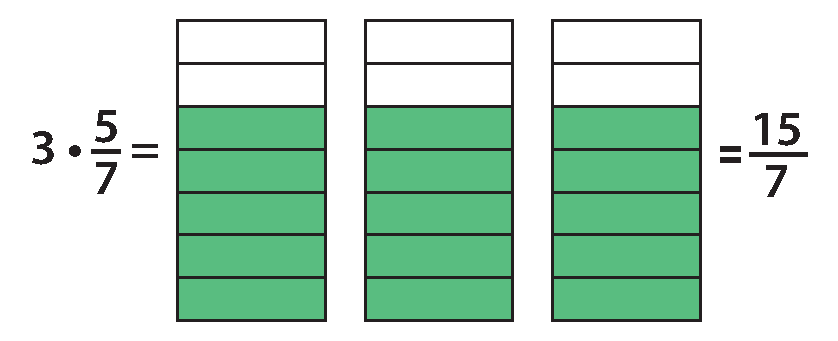
\includegraphics[scale=0.4]{pictures/Kuva3-1-1.pdf}
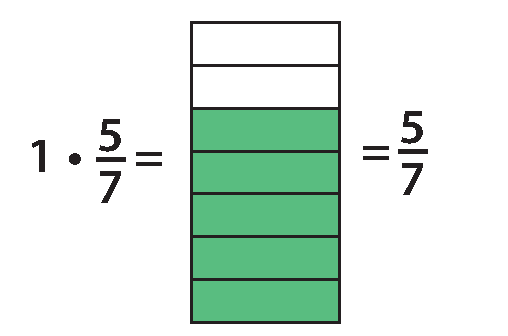
\includegraphics[scale=0.4]{pictures/Kuva3-1-2.pdf}
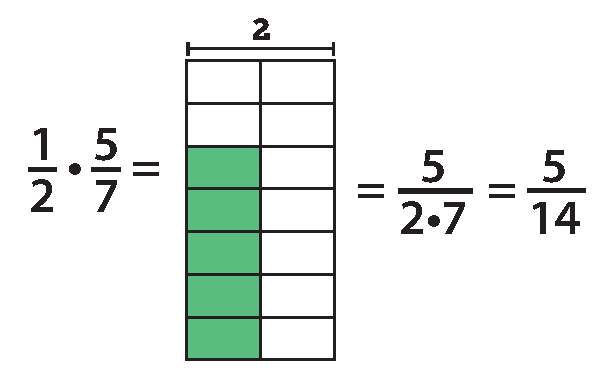
\includegraphics[scale=0.4]{pictures/Kuva3-1-3.pdf}
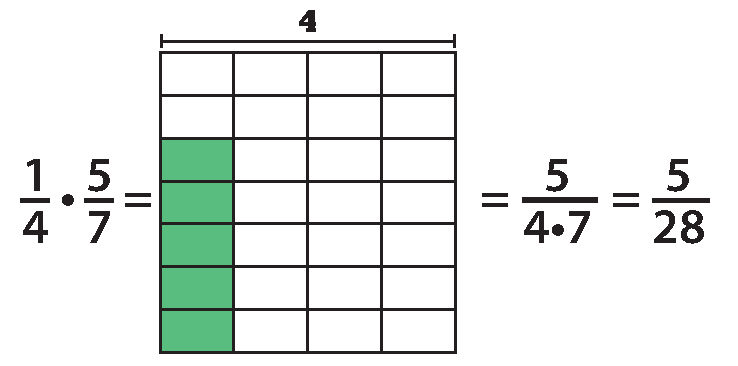
\includegraphics[scale=0.4]{pictures/Kuva3-1-4.pdf}
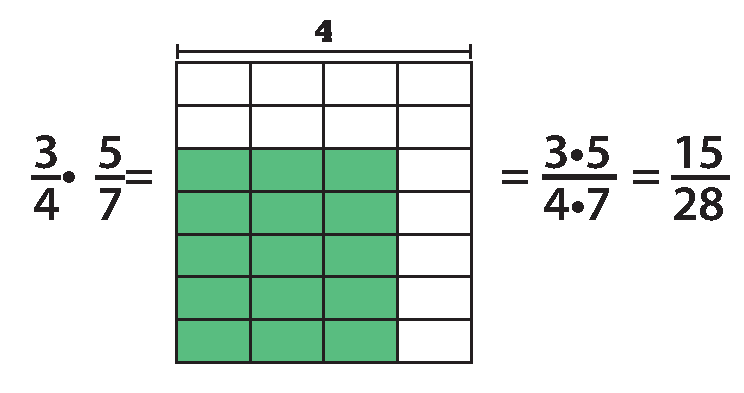
\includegraphics[scale=0.4]{pictures/Kuva3-1-5.pdf}

\begin{esimerkki}
	Luvun $5$ \emph{käänteisluku} on $\frac{1}{5}$, koska
	\[
	 5\cdot \frac{1}{5}=1.
	\]
	Vastaavasti luvun $-\frac{2}{3}$ käänteisluku on $-\frac{3}{2}$, koska
	\[
	 -\frac{2}{3}\cdot (-\frac{3}{2})=1.
	\]

\end{esimerkki}
\laatikko{
    Rationaaliluvun $a$ ($a\neq 0$) \emph{käänteisluku} on  $\frac{1}{a}$, sillä
    \[
    a\cdot \frac{1}{a} = 1.
    \]
    Vastaavasti rationaaliluvun $\frac{a}{b}$ ($a\neq 0$ ja $b\neq 0$) käänteisluku on $\frac{b}{a}$, sillä
    \[
    \frac{a}{b}\cdot \frac{b}{a} = 1.
    \]    

  %  Murtolukujen $p=\frac{a}{b}$ ja $q=\frac{c}{d}\neq 0$ \emph{osamäärä} $p : q$ saadaan, kun kerrotaan luku $p$ luvun $q$ käänteisluvulla,
 %   \[
 %\frac{p}{q} = p\cdot q^{-1} = \frac{a}{b}\cdot\Big(\frac{c}{d}\Big)^{-1} = \frac{a}{b}\cdot \frac{d}{c}
 %   = \frac{ad}{bc}.
 %  \]
 }
    \textbf{Kun vertailet kahta murtolukua, lavenna ne ensin samannimisiksi.}
    
    \begin{esimerkki}
        Salamipizza jaetaan kuuteen ja tonnikalapizza neljään yhtä suureen
        siivuun. Vesa saa kaksi siivua salamipizzaa ja yhden siivun tonnikalapizzaa.
        Minttu saa kaksi siivua tonnikalapizzaa. Kumpi saa enemmän pizzaa, jos
        molemmat pizzat ovat saman kokoisia?
        
        \begin{center}        
          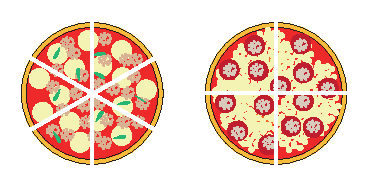
\includegraphics[scale=1.0]{pictures/Kuva3-1-6-pizzat.pdf}
        \end{center}

        \textbf{Ratkaisu.}
        
        Huomataan, että $12 = 3\cdot 4 = 2\cdot 6$. Luvut kannattaa
        pizzan kokonaismäärän laskemista varten laventaa niin, että
        nimittäjänä on luku $12$.
        Vesan saama määrä pizzaa on
        \begin{align*}
           \frac{2}{6} + \frac{1}{4} &= \frac{2\cdot 2}{2\cdot 6} + \frac{3\cdot 1}{3\cdot 4} \\ 
	       							 &= \frac{4}{12}+\frac{3}{12} \\ 
	       							 &= \frac{7}{12}.
        \end{align*}
        
        Mintun saama määrä pizzaa on
        \[
            \frac{2}{4} =
            \frac{3\cdot 2}{3\cdot 4} =
            \frac{6}{12}.
        \]
        Koska $6/12 < 7/12$, Vesa saa enemmän.
    \end{esimerkki}
    
    Kaikki rationaaliluvut voidaan esittää murtolukumuodossa, mutta myös
    kokonaisluvut voidaan esittää murtolukuina asettamalla murtoluvun
    nimittäjäksi yksi. Tätä voidaan käyttää, kun lasketaan yhteen
    kokonaislukuja ja murtolukuja.
    
    \begin{esimerkki}
        Laske
        \[
            2 + \frac{1}{3}.
        \]
        
        \textbf{Ratkaisu.}
        
%        Kirjoitetaan aluksi
%        \[
%            2=\frac{2}{1}.
%        \]
		Kirjoitetaan lausekkeen kokonaisluku $2$ murtolukuna, jonka
		jälkeen voidaan murtoluvut voidaan laventaa samannimisiksi
		ja laskea yhteen:
        \begin{align*}
           2 + \frac{1}{3} &= \frac{2}{1} + \frac{1}{3}  \\ 
	       				   &= \frac{3 \cdot 2}{3 \cdot 1} + \frac{1}{3} \\ 
	       				   &= \frac{6+1}{3} \\ 
	       				   &= \frac{7}{3}.
        \end{align*}
    \end{esimerkki}
    

    
%%%anonyymiltä lahjoittajalta

\begin{tehtavasivu}

\subsubsection*{Opi perusteet}

%     vanha sivulaatikko
%    \laatikko{
%	Laskujärjestys:
%        \begin{enumerate}
%            \item Sulut
%            \item Potenssilaskut
%            \item Kerto- ja jakolaskut vasemmalta oikealle
%            \item Yhteen- ja jakolaskut vasemmalta oikealle
%        \end{enumerate}
%    }

\begin{tehtava}
Supista. \quad
a) $\frac{15}{20}$ \qquad b) $\frac{14}{21}$ \qquad c) $\frac{12}{20}$
\begin{vastaus}
a) $\frac{3}{4}$ \qquad b) $\frac{2}{3}$\qquad c) $\frac{3}{5}$
\end{vastaus}
\end{tehtava}

\begin{tehtava}
Lavenna samannimisiksi
\begin{alakohdat}
\alakohta{$\frac{2}{3}$ ja $\frac{4}{5}$} 
\alakohta{$\frac{5}{6}$ ja $\frac{7}{9}$}
\alakohta{$\frac{2}{3}$ ja $\frac{7}{2}$}
\end{alakohdat}
\begin{vastaus}
\begin{alakohdat}
\alakohta{$\frac{10}{15}$ ja $\frac{12}{15}$}
\alakohta{$\frac{15}{18}$ ja $\frac{14}{18}$}
\alakohta{$\frac{4}{6}$ ja $\frac{21}{6}$}
\end{alakohdat}
\end{vastaus}
\end{tehtava}

\begin{tehtava}
Laske.
	\begin{alakohdat}
		\alakohta{$\frac{3}{11}+\frac{5}{11}$}
		\alakohta{$\frac{4}{5}-\frac{1}{5}$}
		\alakohta{$\frac{2}{3}+\frac{1}{6}$}
		\alakohta{$ \frac{11}{12}-\frac{5}{6}$}
	\end{alakohdat}
	\begin{vastaus}
		\begin{alakohdat}
			\alakohta{$\frac{8}{11}$}
			\alakohta{$\frac{3}{5}$}
			\alakohta{$\frac{5}{6}$}
			\alakohta{$\frac{1}{12}$}
		\end{alakohdat}
	\end{vastaus}
\end{tehtava}

\begin{tehtava}
Muuta sekamurtoluvuksi 
%täsmällisemmin sekamurtolukumuotoon, mutta pienellä piirillä 
% ajateltiin, että tämä epätäsmällinen muotoilu parempi
\begin{alakohdat}
\alakohta{$\frac{15}{2}$} 
\alakohta{$\frac{9}{4}$}
\alakohta{$\frac{23}{7}$}
\end{alakohdat}
\begin{vastaus}
\begin{alakohdat}
\alakohta{$7\frac{1}{2}$}
\alakohta{$2\frac{1}{4}$}
\alakohta{$3\frac{2}{7}$}
\end{alakohdat}
\end{vastaus}
\end{tehtava}

\begin{tehtava}
Muunna murtoluvuksi 
\begin{alakohdat}
\alakohta{$3\frac{2}{5}$}
\alakohta{$4\frac{1}{3}$}
\alakohta{$2\frac{6}{7}$}
\end{alakohdat}
\begin{vastaus}
\begin{alakohdat}
\alakohta{$\frac{17}{5}$}
\alakohta{$\frac{13}{12}$}
\alakohta{$\frac{20}{7}$}
\end{alakohdat}
\end{vastaus}
\end{tehtava}

\begin{tehtava}
Laske.
	\begin{alakohdat}
		\alakohta{$1\frac{2}{9}+\frac{5}{9}$}
		\alakohta{$\frac{1}{3}+2\frac{1}{3}$}
		\alakohta{$2+\frac{5}{4}$}
		\alakohta{$ \frac{3}{2}-\frac{5}{6}$}
	\end{alakohdat}
	\begin{vastaus}
		\begin{alakohdat}
			\alakohta{$\frac{16}{9}$}
			\alakohta{$\frac{8}{3}$}
			\alakohta{$\frac{13}{4}$}
			\alakohta{$\frac{2}{3}$}
		\end{alakohdat}
	\end{vastaus}
\end{tehtava}

\begin{tehtava}
Laske.
	\begin{alakohdat}
		\alakohta{$\frac{2}{3}\cdot \frac{4}{5}$}
		\alakohta{$\frac{3}{5} \cdot \frac{5}{4}$}
		\alakohta{$3\cdot \frac{2}{7}$}
		\alakohta{$\frac{4}{5}\cdot 5$}
	\end{alakohdat}
	\begin{vastaus}
		\begin{alakohdat}
			\alakohta{$\frac{8}{15}$}
			\alakohta{$\frac{15}{20}=\frac{3}{4}$}
			\alakohta{$\frac{6}{7}$}
			\alakohta{$4$ (koska $\frac{20}{5}=4$)}
		\end{alakohdat}
	\end{vastaus}
\end{tehtava}


\begin{tehtava}
a) $\frac{2}{3} : \frac{7}{11}$ \qquad b) $\frac{4}{3}:(\frac{-13}{4})$ \qquad c) $\frac{7}{8}:4$
\begin{vastaus}
a) $1\frac{1}{21}$ \qquad b) $-\frac{16}{39}$ \qquad c) $\frac{7}{32}$
\end{vastaus}
\end{tehtava}

\subsubsection*{Hallitse kokonaisuus}

\begin{tehtava}
Laske murtolukujen $\frac{5}{6}$ ja $-\frac{2}{15}$ \\ a) summa \qquad b) erotus \qquad c) tulo \qquad d) osamäärä.
\begin{vastaus}
a) $\frac{7}{10}$ \qquad b) $\frac{29}{30}$ \qquad c) $-\frac{1}{9}$ \qquad d) $-6\frac{1}{4}$
\end{vastaus}
\end{tehtava}

\begin{tehtava}
a) $\frac{5}{8}\cdot(\frac{3}{5}+\frac{2}{5})$ \qquad b) $\frac{1}{3}+\frac{1}{4}\cdot\frac{6}{5}$
\begin{vastaus}
a) $\frac{5}{8}$ \qquad b) $\frac{19}{30}$
\end{vastaus}
\end{tehtava}

\begin{tehtava}
a) $\dfrac{\frac{1}{2}:\frac{3}{2}}{\frac{3}{2}+\frac{1}{3}}$ \qquad b) $\dfrac{\frac{2}{3}+\frac{3}{4}}{\frac{5}{6}-\frac{7}{12}}$.
\begin{vastaus}
a) $\frac{2}{11}$ \qquad b) $5\frac{2}{3}$
\end{vastaus}
\end{tehtava}

\begin{tehtava} 
        Laatikossa on palloja, joista kolmasosa on mustia, neljäsosa
        valkoisia ja viidesosa harmaita. Loput palloista ovat 		 	punaisia.
        Kuinka suuri osuus palloista on punaisia?
        
        \begin{vastaus}
            $1-(\frac{1}{3}+\frac{1}{4}+\frac{1}{5})
            = \frac{60}{60}-\frac{20}{60}-\frac{15}{60}-\frac{12}{60}
            = \frac{60}{60}-\frac{47}{60}
            = \frac{13}{60}$
        \end{vastaus}
    \end{tehtava}

\begin{tehtava}
Laske lausekkeen $\frac{x}{2-3x}$ arvo, kun $x$ on \\ a) 4 \qquad b) $-\frac{1}{2}$ \qquad c) $\frac{7}{10}$.
\begin{vastaus}
a) $-\frac{2}{5}$ \qquad b) $-\frac{1}{7}$ \qquad c) $-7$
\end{vastaus}
\end{tehtava}


\subsubsection*{Lisää tehtäviä}

\begin{tehtava}
Laske lausekkeen $\frac{x+y}{2x-y}$ arvo, kun \\ a) $x=\frac{1}{2}$ ja $y= \frac{1}{4}$ \qquad b) $x=\frac{1}{4}$ ja $y= -\frac{3}{8}$.
\begin{vastaus}
a) $1$ \qquad b) $-\frac{1}{7}$
\end{vastaus}
\end{tehtava}


 %   Yksi prosentti tarkoittaa yhtä sadasosaa: $1~\% = \frac{1}{100}$
 
 %TODO pitäisikö selittää leipätekstissä ja antaa joku esimerkki?
    
        \begin{tehtava}
            \begin{enumerate}[a)]
        	\item $\frac{3}{5} + \frac{1}{5}$
        	\item $\frac{5}{7} + \frac{4}{7}$
        	\item $2 + \frac{2}{3}$
        	\item$3 + \frac{3}{5} + \frac{2}{5}$   
            \end{enumerate}
            \begin{vastaus}
        		\begin{enumerate}[(a)]
        			\item $\frac{4}{5}$
        			\item $\frac{9}{7} = 1 \frac{2}{7}$
        			\item $2 \frac{2}{3} = \frac{8}{3}$
        			\item $4$
        		\end{enumerate}
            \end{vastaus}
        \end{tehtava}
        
        \begin{tehtava}
        
        \begin{enumerate}[a)]
        	\item $\frac{6}{2} + \frac{3}{5}$
        	\item $\frac{7}{8} - \frac{1}{4}$
        	\item $2 \frac{1}{3} + \frac{4}{6}$
        	\item $4 \frac{7}{2} - 6 \frac{5}{4}$
        \end{enumerate}
            \begin{vastaus}		
        		\begin{enumerate}[a)]
        			\item $\frac{18}{5}$
        			\item $\frac{5}{8}$
        			\item $3$
        			\item $-\frac{41}{6}$ 
        		\end{enumerate}
            \end{vastaus}
        \end{tehtava}
        
        \begin{tehtava}
        
        \begin{enumerate}[a)]
        	\item $2 \cdot \frac{2}{5}$
        	\item $2 \cdot \frac{2}{3}$
        	\item $\frac{5}{4} \cdot 2 \cdot 3$
        	\item $\frac{\frac{3}{7}}{4}$ 
        \end{enumerate}
            \begin{vastaus}
        		\begin{enumerate}[a)]
        			\item $\frac{4}{5}$
        			\item $\frac{4}{3} = 1 \frac{1}{3}$
        			\item $\frac{15}{2} = 7 \frac{1}{2}$
        			\item $\frac{3}{28}$
        		\end{enumerate}
            \end{vastaus}
        \end{tehtava}
        
        \begin{tehtava}
        
        \begin{enumerate}[a)]
        	\item $\frac{1}{3} \cdot \frac{6}{5}$
        	\item $\frac{5}{4} \cdot (-\frac{2}{3})$ 
        	\item $\frac{2}{5} (2 - \frac{3}{4})$
        	\item $(\frac{5}{6} - \frac{1}{3})(\frac{7}{4} - \frac{3}{2})$
        \end{enumerate}
            \begin{vastaus}		
        		\begin{enumerate}[a)]
        			\item $\frac{2}{5}$
        			\item $-\frac{5}{6}$
        			\item $\frac{1}{2}$
        			\item $\frac{1}{8}$ 
        		\end{enumerate}
            \end{vastaus}
        \end{tehtava}
        
        \begin{tehtava}
        
        \begin{enumerate}[a)]
        	\item $\displaystyle \frac{\frac{3}{7} + \frac{5}{4}}{3}$
        	\item $\displaystyle \frac{\frac{10}{8}}{\frac{5}{2}}$
        	\item $\displaystyle \frac{\frac{1}{3} - \frac{5}{10}}{\frac{3}{4} + \frac{1}{2}}$
        	\item $\displaystyle 3\frac{\frac{4}{2} + \frac{10}{4}}{\frac{3}{2} - \frac{2}{3}}$
        \end{enumerate}
            \begin{vastaus}		
        		\begin{enumerate}[a)]
        			\item $\frac{47}{28}$
        			\item $\frac{1}{2}$
        			\item $-\frac{1}{3}$
        			\item $\frac{54}{5}$
        		\end{enumerate}
            \end{vastaus}
        \end{tehtava}
    
    \begin{tehtava} %syvteht
        Pontus, Viljami, Jarkko-Kaaleppi, Simo ja Milla leipoivat lanttuvompattipiirakkaa.
        Pontus kuitenkin söi piirakasta kolmanneksen ennen muita, ja loput piirakasta
        jaettiin muiden kanssa tasan. Kuinka suuren osan muut saivat?
        
        \begin{vastaus}
            Muut saivat piirakasta kuudesosan.
        \end{vastaus}
    \end{tehtava}
    
    \begin{tehtava} %perusteht
        Huvipuiston sisäänpääsylippu maksaa 20 euroa, ja lapset pääsevät
        sisään puoleen hintaan.
	\begin{enumerate}[a)]
		\item Kuinka paljon kolmen lapsen yksinhuoltajaperheelle maksaa päästä sisään?
		\item Kuinka paljon sisäänpääsy maksaa perheelle avajaispäivänä,
		kun silloin sisään pääsee 25~\% halvemmalla?
        \end{enumerate}
        \begin{vastaus}
	\begin {enumerate}[a)]
         \item 50 euroa 
           \item 50 euroa 
	\item 37,50 euroa
\end{enumerate} 
       \end{vastaus}
    \end{tehtava}  
  
    \begin{tehtava}
        Laske 
        $\frac{10}{9}\cdot \frac{9}{8}\cdot \frac{8}{7}\cdot \frac{7}{6}\cdot \frac{6}{5}
            \cdot \frac{5}{4}\cdot \frac{4}{3}\cdot \frac{3}{2}$.
        
        \begin{vastaus}
            $\frac{10}{2}=5$.
        \end{vastaus}        
    \end{tehtava}
    
    \begin{tehtava}
    	Eräässä kaupassa on käynnissä loppuunmyynti, ja kaikki tuotteet
        myydään puoleen hintaan. Lisäksi kanta-asiakkaat saavat aina
        viidenneksen alennusta tuotteiden senhetkisestä hinnasta.
    	Paljonko kanta-asiakas maksaa nyt tuotteesta, joka normaalisti
        maksaisi 40 euroa?
    	\begin{vastaus}
    	$40\cdot \frac{1}{2} \cdot \frac{4}{5}=40\cdot \frac{4}{10}= 16$. 
    	\end{vastaus}
    \end{tehtava}
    
    \begin{tehtava}
        Kokonaisesta kakusta syödään maanantaina iltapäivällä puolet, ja jäljelle
        jääneestä palasta syödään tiistaina iltapäivällä taas puolet.
        Jos kakun jakamista ja syömistä jatketaan samalla tavalla koko viikko,
        kuinka suuri osa alkuperäisestä kakusta on
        jäljellä seuraavana maanantaiaamuna?
        
        \begin{vastaus}
            Toisena päivänä aamulla kakkua on jäljellä puolet, kolmantena
            päivänä aamulla
                $1-\left(\frac{1}{2} + \frac{1}{4}\right) = \frac{1}{4}$, 
            neljäntenä päivänä
                $1-\left(\frac{1}{2} + \frac{1}{4} + \frac{1}{8}\right)
                = \frac{1}{8}$, jne.
            Siis seitsemän päivän jälkeen kakkua on jäljellä
                $1-\left(\frac{1}{2} + \frac{1}{4} + \frac{1}{8} +
                \frac{1}{16} + \frac{1}{32} + \frac{1}{64} + \frac{1}{128}\right)
                = \frac{1}{128}$.  
        \end{vastaus}
    \end{tehtava}

    \begin{tehtava} %syvteht
Ratkaise lausekkeen $\frac{1}{n}-\frac{1}{m}$ arvo, kun tiedetään, että $n = \frac{1}{6}$ ja $m=n+1$.
        \begin{vastaus}
            $5 \frac{1}{7}$
        \end{vastaus}
    \end{tehtava}


\begin{tehtava}
a) $\frac{4}{9} : \frac{1}{5}$ \qquad b) $\frac{2}{7}:\frac{5}{9}$ \qquad c) $\frac{2}{3}:\frac{4}{3}$
\begin{vastaus}
a) $\frac{20}{9}$ \qquad b) $\frac{18}{35}$ \qquad c) $\frac{1}{2}$
\end{vastaus}
\end{tehtava}

\begin{tehtava}
$\star$ Fibonaccin luvut 0, 1, 1, 2, 3, 5, 8, 13, 21, $\ldots$ määritellään seuraavasti: Kaksi ensimmäistä
Fibonaccin lukua ovat 0 ja 1, ja siitä seuraavat saadaan kahden
edellisen summana: 
\[ 0+1=1, \quad 1+1=2, \quad 1+2 = 3, \quad 2+3=5 \] 
ja niin edelleen. 
Tutki, miten Fibonaccin luvut liittyvät lukuihin
\[ \frac{1}{1+1}, \quad \frac{1}{1+\frac{1}{1+1}}, \quad
\frac{1}{1+\frac{1}{1+\frac{1}{1+1}}}, \quad 
\frac{1}{1+\frac{1}{1+\frac{1}{1+\frac{1}{1+1}}}}, \quad \ldots\]
\begin{vastaus}
Luvut ovat sievennettynä peräkkäisten Fibonaccin
lukujen osamääriä:
\[\frac{1}{2}, \ \frac{2}{3}, \ \frac{3}{5}, \frac{5}{8} \ldots  \]
\end{vastaus}
\end{tehtava}


\end{tehtavasivu}
    \section{Potenssi}
    
    Jos $a$ on reaaliluku ja $n$ on positiivinen kokonaisluku, potenssilla $a^n$ tarkoitetaan tuloa
    \[
        a^n = \underbrace{a\cdot \ldots \cdot a}_{n\text{ kpl}}. 
    \]
Lukua $a$ kutsutaan potenssin \emph{kantaluvuksi} ja lukua $n$ \emph{eksponentiksi}. Merkinnällä $2^4$ siis tarkoitetaan tuloa $2\cdot 2\cdot 2\cdot 2$. Siten
        \[
            2^4=2\cdot 2\cdot 2\cdot 2=16.
        \]
Luvun toista potenssia $a^2$ kutsutaan myös luvun $a$ \emph{neliöksi} ja kolmatta potenssia $a^3$ sen \emph{kuutioksi}. Luvun $a>0$ neliö on sellaisen neliön pinta-ala, jonka sivun pituus on $a$. Vastaavasti, jos kuution särmän pituus on $a$, on $a^3$ kyseisen kuution tilavuus.  
            
    \begin{esimerkki}
        Potenssien sieventäminen.
        \begin{enumerate}[a)]
            \item $(-2)^3 = (-2)\cdot (-2)\cdot (-2) = -8$
            \item $(-2)^4 = (-2)\cdot (-2)\cdot (-2)\cdot (-2) = 16$
            \item $-2^4   = -(2^4) = -(2\cdot 2\cdot 2\cdot 2) = -16$
            \item $2^2\cdot 2^3 =
                \underbrace{2\cdot 2}_{\text{$2$ kpl}}\cdot \underbrace{2\cdot
                2\cdot 2}_{\text{$3$ kpl}} = \underbrace{2\cdot 2\cdot 2\cdot 2\cdot 2}_{\text{$5$ kpl}}=2^5 = 32$
            \item $\displaystyle\frac{2^4\cdot 2^2}{2^3} =
                \frac{2\cdot 2\cdot 2\cdot \cancel{2} \cdot \cancel{2}\cdot
                \cancel{2}}{\cancel{2}\cdot \cancel{2}\cdot \cancel{2}} = 2^3 = 8$
        \end{enumerate}
    \end{esimerkki}
    
\subsection*{Potenssien laskusäännöt}
    
    Samankantaisten potenssien kertolasku
	\[
a^3\cdot a^4=\underbrace{a\cdot a\cdot a}_{\text{3 kpl}}\cdot \underbrace{a\cdot a\cdot a\cdot a}_{\text{4kpl}}=a^{\mathbf{3+4}}=a^7
    	\]
    Samankantaisten potenssien jakolasku
	\[
\frac{a^7}{a^4}=\frac{a\cdot a\cdot a\cdot \cancel{a}\cdot \cancel{a}\cdot \cancel{a}\cdot \cancel{a}}	{\cancel{a}\cdot \cancel{a}\cdot \cancel{a}\cdot \cancel{a}}=a^{\mathbf{7-4}}=a^3
    	\]
    Potenssin potenssi
	\[
(a^2)^3=\underbrace{a^2\cdot a^2\cdot a^2}_{3\text{ kpl}}=\underbrace{a\cdot a\cdot a\cdot a\cdot a\cdot a}_{2\cdot 3=6\text{ kpl}}=a^{\boldsymbol{{2\cdot 3}}}=a^6
\]
    Tulon potenssi
	\[
(ab^5)^3=ab^5\cdot ab^5\cdot ab^5=a\cdot a\cdot a\cdot b^5\cdot b^5\cdot b^5=a^{\mathbf{1\cdot 3}}\cdot b^{\mathbf{5\cdot 3}}=a^3b^{15}
	\]
     Osamäärän potenssi
	\[
	\left(\frac{a^9}{b^7}\right)^3=\frac{a^9}{b^7}\cdot \frac{a^9}{b^7}\cdot \frac{a^9}{b^7}=\frac{a^9\cdot a^9\cdot a^9}{b^7\cdot b^7\cdot b^7}=\frac{a^{\mathbf{9\cdot 3}}}{b^{\mathbf{7\cdot 3}}}=\frac{a^{27}}{a^{21}}
	\]

    Potensseille pätevät seuraavat laskusäännöt.
    
    \laatikko{
        \textbf{Potenssien laskusääntöjä}
    
        Olkoot $m$ ja $n$ kokonaislukuja ja $a$ reaaliluku.
        
        \begin{tabular}{ll}
            $a^m\cdot a^n            = a^{m+n}$ & Samakantaisten potenssien tulo\\ % Kielitoimiston sanakirjan mukaan samakantainen, ei samankantainen
            $\displaystyle \frac{a^m}{a^n}= a^{m-n}$ & Samakantaisten potenssien osamäärä ($a\neq 0$)\\
            $(a\cdot b)^n            = a^n\cdot b^n$ & Tulon potenssi\\
            $\displaystyle \left (\frac{a}{b}\right)^n = \frac{a^n}{b^n}$ & Osamäärän potenssi ($b\neq 0$)\\ 
            $(a^m)^n                 = a^{m\cdot n}$ & Potenssin potenssi\\
        \end{tabular}
    }
    
\subsection*{Negatiivinen luku ja nolla eksponenttina}
    
    Sievennetään osamäärä $\frac{a^3}{a^5}$ kahdella eri tavalla. Supistamalla yhteiset tekijät lopputulos
    
    \begin{equation*}
        \frac{a^3}{a^5} =
        \frac{\cancel{a}\cdot \cancel{a}\cdot \cancel{a}}{a\cdot a\cdot
        \cancel{a}\cdot \cancel{a}\cdot \cancel{a}} = 
        \frac{1}{a\cdot a}=\boldsymbol{\frac{1}{a^2}}
    \end{equation*}
    
    on erinäköinen, kuin käyttämällä potenssien laskusääntöjä
    
    \begin{equation*}
        \frac{a^3}{a^5} = a^{3-5}=\boldsymbol {a^{-2}}{.}
    \end{equation*}
    
    Koska lähtötilanne on molemmissa tapauksissa sama, voidaan määritellä, että
    
    \begin{equation*}
        a^{-2} = \frac{1}{a^2}
    \end{equation*}
  
    \laatikko{
        \textbf {Negatiivinen eksponentti} (kun $a\neq 0$)
        \begin{equation*}
        	a^{-n} = \frac{1}{a^n}
        \end{equation*}
    }
    
    Kun eksponenttina on nolla, on tuloksena aina luku $1$ kaikilla nollasta poikkeavilla kantaluvuilla. 
    Esimerkiksi
    \[
        \frac{a^3}{a^3}=\frac{\cancel{a}\cdot \cancel{a}\cdot \cancel{a}}{\cancel{a}\cdot \cancel{a}\cdot \cancel{a}}=1,
    \]
    mutta sama lasku voidaan laskea myös toisella tavalla: $\frac{a^3}{a^3}=a^{3-3}=a^0$.
  
    \laatikko{
        \textbf{Eksponenttina nolla} (kun $a\neq 0$)
        \begin{equation*}
            a^{0}=1
        \end{equation*}
    }

Merkintää $0^0$ ei ole määritelty.    

%    \subsection*{Laskujärjestys}
%    
%    \laatikko{
%        \begin{enumerate}
%            \item Sulut
%            \item Potenssilaskut
%            \item Kerto- ja jakolaskut vasemmalta oikealle
%            \item Yhteen- ja jakolaskut vasemmalta oikealle
%        \end{enumerate}
%    }
%   

\paragraph*{Huomautus laskujärjestyksestä}

Mikäli potensseja on monta päällekkäin (eli eksponenttina on potenssilauseke),
laskeminen aloitetaan ylimmästä potenssista. Esimerkiksi
\[2^{3^2}= 2^9 = 512. \]
Laskujärjestystä voidaan muuttaa suluilla:
\[(2^3)^2=8^2=64. \]

\subsection*{Tehtäviä}

\paragraph*{Opi perusteet}

    \begin{tehtava}
        Laske. \quad
        a) $(-2)\cdot(-2)\cdot(-2)$ \qquad
        b) $(-1)\cdot(-1)\cdot(-1)\cdot(-1)$

        \begin{vastaus}
            a) $ -8$ \qquad
            b) $1$
        \end{vastaus}
    \end{tehtava}

    \begin{tehtava}
        Sievennä. \quad
        a) $a\cdot a\cdot a$ \quad
        b) $a\cdot a\cdot a\cdot b\cdot b\cdot b\cdot b$ \quad
        c) $a\cdot b\cdot a\cdot b\cdot a\cdot b\cdot a$
        
        \begin{vastaus}
            a) $a^3$ \qquad
            b) $a^3b^4$ \qquad
            c) $a^4b^3$
        \end{vastaus}
    \end{tehtava}


    \begin{tehtava}
        Laske. \quad
        a) $2^3\cdot2^3$ \qquad
        b) $4^3$ \qquad
        c) $(2^2)^3$ \qquad
        d) $2^{2+2+2}$

        \begin{vastaus}
            a) $64$ \qquad
            b) $64$ \qquad
            c) $64$ \qquad
            d) $64$
        \end{vastaus}
    \end{tehtava}

\begin{tehtava}
        Sievennä. \quad \
        a) $a^3\cdot a^2\cdot a^5$ \quad \
        b) $(a^3)^2$ \quad \
        c) $(a^2a^3)^4$ \quad \
        d) $a^{7-2}$

        \begin{vastaus}
            a) $a^{10}$ \qquad
            b) $a^6$ \qquad
            c) $a^{20}$ \qquad
            d) $a^5$
        \end{vastaus}
    \end{tehtava}

  \begin{tehtava}
        Laske. \quad
        a) $\displaystyle \frac{2^3}{2^2}$ \quad \
        b) $\displaystyle \frac{2^4}{2^2}$ \quad \
        c) $\displaystyle \frac{2^3}{2^1}$ \quad \
        d) $\displaystyle \frac{2^3}{2^0}$ \quad \
        e) $\displaystyle \frac{2^3}{2^4}$ \quad \
        f) $\displaystyle \frac{2^3}{2^5}$
        
        \begin{vastaus}
            a) $2$ \qquad
            b) $4$ \qquad
            c) $4$ \qquad
            d) $8$ \qquad
            e) $\frac{1}{2}$ \qquad
            f) $\frac{1}{4}$
        \end{vastaus}
    \end{tehtava}

\paragraph*{Hallitse kokonaisuus}

Sievennä.

 \begin{tehtava}
        %Sievennä. \quad
        a) $(1\cdot a)^3$ \qquad
        b) $(a\cdot 2)^2$ \qquad
        c) $(-2abc)^3$ \qquad
        d) $(3a)^4$

        \begin{vastaus}
            a) $a^3$ \qquad
            b) $4a^2$ \qquad
            c) $-8a^3b^3c^3$ \qquad
            d) $91a^4$
        \end{vastaus}
    \end{tehtava}


 \begin{tehtava}
        %Sievennä. \quad
        a) $a^3\cdot b^2\cdot a^5$ \qquad 
        b) $(-ab^3)^2$ \qquad 
        c) $(a^5a^4)^3$ \qquad 
        d) $10^{2^3}$

        \begin{vastaus}
            a) $a^8b^2$ \qquad
            b) $a^2b^6$ \qquad
            c) $a^{15}b^{12}$ \qquad
            d) $10^8 = 100~000~000$
        \end{vastaus}
    \end{tehtava}

    \begin{tehtava}
        %Sievennä. \quad
        a) $(-a)\cdot(-a)$ \qquad
        b) $(-a)\cdot(-a)\cdot(-b)^3$ \qquad
        c) $(-a^2)\cdot(-a)^2$

        \begin{vastaus}
            a) $a^2$ \qquad
            b) $-a^2b^3$ \qquad
            c) $-a^4$
        \end{vastaus}
    \end{tehtava}

 \begin{tehtava}
        %Sievennä. \quad
        a) $b^3(ab^0)^2$ \qquad
        b) $(ab^3)^0$ \qquad
        c) $(aa^4)^3a^2$ \qquad
        d) $a^3(b^2a)^5$

        \begin{vastaus}
            a) $a^2b^3$ \qquad
            b) $1$ \qquad
            c) $a^{17}$ \qquad
            d) $a^8b^{10}$
        \end{vastaus}
    \end{tehtava}

 \begin{tehtava}
        %Sievennä. \quad
        a) $(\frac{1}{2})\cdot(\frac{1}{2})$ \qquad
        b) $(-\frac{ab^2}{a^2b})^3$ \qquad
        c) $(-a^4b^4)^2$ \qquad
        d) $\left((\frac{a}{b})^4\right)^2$
        
        \begin{vastaus}
            a) $\frac{1}{4}$ \qquad
            b) $-\frac{b^3}{a^3}$ \qquad
            c) $a^8b^8$ \qquad
            d) $\frac{a^8}{b^8}$
        \end{vastaus}
    \end{tehtava}
    
    \begin{tehtava}
        %Sievennä. \quad
        a) $\frac{6a^9}{3a^2}$ \qquad
        b) $(\frac{a^2b^{-2}}{a^2b})^{-3}$ \qquad
        c) $\frac{5a^2}{-15a}$ \qquad
        d) $\left(-(\frac{10^3}{100b})^2 b^{-1} \right )^2$
        
        \begin{vastaus}
            a) $2a^7$ \qquad
            b) $b^9$ \qquad
            c) $-\frac{1}{3}a = -\frac{a}{3}$ \qquad
            d) $\frac{10~000}{b^6}$
        \end{vastaus}
    \end{tehtava}

\begin{tehtava}
$\boldsymbol{[\star]}$ Tetraatio on lyhennysmerkintä ''potenssitornille'',
jossa esiintyy vain yhtä lukua. Se määritellään seuraavasti.
\[^na = \underbrace{{a^{a^{a^{\mathstrut^{.^{.^{.^{a}}}}}}}}}_{n\textrm{ kpl }}. \]
Laske \quad a) $^42$  \quad b) $^35$. \quad c) Ratkaise yhtälö $^x2= 16$.
\begin{vastaus}
a) $^42 = 2^{2^{2^2}}=2^{2^4}=2^{16}=65\ 536$ \
b) $^35 = 5^{5^5} = 5^{25} \approx 2,98 \cdot 10^{17}$. \\
c) Kokeilemalla $x =3$.
\end{vastaus}
\end{tehtava}

\paragraph*{Sekalaisia tehtäviä}

%%%%%%%%%%%%%%%%%%%%%%%%%%%%%%%%%%
      Sievennä.
    
    \begin{tehtava}
        %Sievennä \quad
        a) $a^2\cdot a^3$ \qquad
        b) $a^3a^2$ \qquad
        c) $a^2 a$ \qquad
        d) $a a^2 a$ \qquad
        e) $a^2a^1a^3$
        
        \begin{vastaus}
            a) $a^5$ \qquad
            b) $a^5$ \qquad
            c) $a^3$ \qquad
            d) $a^4$ \qquad
            e) $a^6$
        \end{vastaus}
    \end{tehtava}
    
    \begin{tehtava}
        %Sievennä \quad
        a) $a^0$ \qquad
        b) $a^0a^0$ \qquad
        c) $a a^1$ \qquad
        d) $aa^0$ \qquad
        e) $a^0a^1$
        
        \begin{vastaus}
            a) $1$ \quad ($a\neq0$, koska $0^0$ ei ole määritelty) \qquad
            b) $1$ \qquad
            c) $a$ \qquad
            d) $a^2$ \qquad
            e) $a$
        \end{vastaus}
    \end{tehtava}
    
    \begin{tehtava}
        %Sievennä \quad
        a) $a^1 a a^2$ \qquad
        b) $aaaa$ \qquad
        c) $a^3ba^2$ \qquad
        d) $aba^0ba^1$
        
        \begin{vastaus}
            a) $ a^4$ \qquad
            b) $a^4$ \qquad
            c) $a^5b$ \qquad
            d) $a^2b^2$
        \end{vastaus}
    \end{tehtava}
    % teht 5
       

    \begin{tehtava}
        %Sievennä \quad
        a) $-a\cdot(-a)$ \qquad
        b) $-a\cdot(-a)\cdot(-b)$ \qquad
        c) $-a^2\cdot(-a^2)$
    
        \begin{vastaus}
            a) $a^2$ \qquad
            b) $-a^2b$ \qquad
            c) $a^4$
        \end{vastaus}
    \end{tehtava}

    \begin{tehtava}
        %Sievennä \quad
        a) $-a^3\cdot(-a^2)$ \qquad
        b) $a\cdot(-a)\cdot(-b)$ \qquad
        c) $a^2\cdot(-a^2)$
        
        \begin{vastaus}
            a) $a^5$ \qquad
            b) $a^2b$ \qquad
            c) $-a^4$
        \end{vastaus}
    \end{tehtava}

    %teht. 10
    \begin{tehtava}
        %Sievennä \quad
        a) $0^3\cdot0^3\cdot0^3$ \qquad
        b) $3^1$ \qquad
        c) $2^{2+3}$ \qquad
        d) $2^{6-4}$ \qquad
        e) $5^0$

        \begin{vastaus}
            a) $0$ \qquad
            b) $3$ \qquad
            c) $32$ \qquad
            d) $4$ \qquad
            e) $1$
        \end{vastaus}
    \end{tehtava}
    \begin{tehtava}
        %Sievennä \quad
        a) $(a^3)^1$ \qquad
        b) $(a^6)^2$ \qquad
        c) $(a^2)^4$ \qquad 
        d) $(a^1)^3$ \qquad
        e) $(a^0)^5$

        \begin{vastaus}
            a) $a^3$ \qquad
            b) $a^{12}$ \qquad
            c) $a^8$ \qquad
            d) $a^3$ \qquad
            e) $1$
        \end{vastaus}
    \end{tehtava}
    
       \begin{tehtava}
        %Sievennä \quad
        a) $(1^3\cdot 2^2)^2$ \qquad
        b) $(1^2\cdot 2^3)^2$ \qquad
        c) $(2^2a^4)^2$ \qquad
        d) $b(3b)^3$

        \begin{vastaus}
            a) $16$ \qquad
            b) $64$ \qquad
            c) $16a^8$ \qquad
            d) $27b^4$
        \end{vastaus}
    \end{tehtava}
    
    \begin{tehtava}
        %Sievennä \quad
        a) $(a^3b^2)^2$ \qquad
        b) $a(a^2b^3)^4$ \qquad
        c) $(b^2a^4)^5$ \qquad
        d) $b(2ab^2)^3$
        
        \begin{vastaus}
            a) $a^6b^4$ \qquad
            b) $a^9b^{12}$ \qquad
            c) $a^{20}b^{10}$ \qquad
            d) $8a^3b^7$
        \end{vastaus}
    \end{tehtava}
      
    \begin{tehtava}
        %Sievennä \quad
        a) $\frac{a^3}{a^2}$ \qquad
        b) $\frac{a^4}{a^2}$ \qquad
        c) $\frac{a^3}{a^1}$ \qquad
        d) $\frac{a^3}{a^0}$ \qquad
        e) $\frac{a^3}{a^4}$ \qquad
        f) $\frac{a^3}{a^5}$
        
        \begin{vastaus}
            a) $a$ \qquad
            b) $a^2$ \qquad
            c) $a^2$ \qquad
            d) $a^3$ \qquad
            e) $a^{-1} = \frac{1}{a}$ \qquad
            f) $a^{-2} = \frac{1}{a^2}$
        \end{vastaus}
    \end{tehtava}
    
    %teht. 20
    \begin{tehtava}
        %Sievennä \quad
        a) $\frac{a^2b^2}{ab}$ \qquad
        b) $\frac{a^2b}{a^2}$ \qquad
        c) $\frac{a^3}{a^3}$ \qquad
        d) $\frac{1}{a^0}$ \qquad
        e) $\frac{ab^3}{-b^4}$
        
        \begin{vastaus}
            a) $ab$ \qquad
            b) $b$ \qquad
            c) $1$ \qquad
            d) $1$ \qquad
            e) $-\frac{a}{b}$
        \end{vastaus}
    \end{tehtava}
    
   
    
    \begin{tehtava}
         Sievennä ja kirjoita potenssiksi, jonka eksponentti on positiivinen.\\
        a) $a^{-3}$ \qquad
        b) $\frac{a}{a^3}$ \qquad
        c) $a^{-2}\cdot a^5$ \qquad
        d) $\frac{b}{a^4}b^{-4}$ \qquad
        e) $\frac{a^3}{a^{-5}}$
        
        \begin{vastaus}
            a) $\frac{1}{a^3}$ \qquad
            b) $\frac{1}{a^2}$ \qquad
            c) $a^3$ \qquad
            d) $\frac{}{a^4b^3}$ \qquad
            e) $a^8$
        \end{vastaus}
    \end{tehtava}
    
    
    
    \begin{tehtava}
        Esitä ilman sulkuja ja sievennä. \\
        a) $(\frac{1}{2})^2$ \qquad
        b) $(\frac{1}{3})^3$ \qquad
        c) $(\frac{a}{b})^4$ \qquad
        d) $(\frac{a^2}{b^3})^2$ \qquad
        e) $\left(\frac{a^2}{ab^2}\right)^2$
        
        \begin{vastaus}
            a) $\frac{1}{4}$ \qquad
            b) $\frac{1}{27}$ \qquad
            c) $\frac{a^4}{b^4}$ \qquad
            d) $\frac{a^4}{b^6}$ \qquad
            e) $\frac{a^2}{b^4}$
        \end{vastaus}
    \end{tehtava}
    % FIXME alla olevat on muotoiltu erilailla (yksi alikohta per rivi).
% Mahtunee samalle riville.
% Lisäksi tässä on duplikaatteja (esim. aaaa:n sievennys on sekä yllä että alla). 
   	Sievennä.
    \begin{tehtava}%perteht
        %Sievennä
		\begin{enumerate}[a)]
        	\item $2^3 $ 
        	\item $aaaa$ 
        	\item $a^3a^2$ 
        	\item $0^4$
		\end{enumerate}        
        \begin{vastaus}
        \begin{enumerate}[a)]
            \item $8$ 
            \item $a^4$ 
            \item $a^5$ 
            \item $0$
        \end{enumerate}
        \end{vastaus}
    \end{tehtava}

    \begin{tehtava}%perteht
        %Sievennä
        \begin{enumerate}[a)]
        	\item $a^2a^5 $ 
        	\item $\frac{a^5}{a^3}$ 
        	\item $(a^3)^2$ 
        	\item $12^0$
		\end{enumerate}        
        \begin{vastaus}
        \begin{enumerate}[a)]
            \item $a^7$ 
            \item $a^2$ 
            \item $a^6$ 
            \item $1$
        \end{enumerate}
        \end{vastaus}
    \end{tehtava}    
    
    %soveltavia tehtäviä
        
    \begin{tehtava}%sovteht
        %Sievennä
        \begin{enumerate}[a)]
        	\item $a^2(-a^4) $ 
        	\item $(ab^2)^0$ 
        	\item $(3a)^3$ 
        	\item $(a^5b^3)^3$
		\end{enumerate}        
        \begin{vastaus}
        \begin{enumerate}[a)]
            \item $-a^6$ 
            \item $1$ 
            \item $27a^3$ 
            \item $a^{15}b^9$
        \end{enumerate}
        \end{vastaus}
    \end{tehtava} 
    
    \begin{tehtava}%sovteht
        %Sievennä
        \begin{enumerate}[a)]
        	\item $\frac{2^7}{2^9}$ 
        	\item $\frac{a^3}{a}$ 
        	\item $\left(\frac{1}{3}\right)^2$ 
        	\item $\left(\frac{a^{-2}}{ab^4}\right)^4$
		\end{enumerate}        
        \begin{vastaus}
        \begin{enumerate}[a)]
            \item $\frac{1}{4}$ 
            \item $a^2$ 
            \item $\frac{1}{9} $ 
            \item $ \left(\frac{1}{a^{12}b^{16}}\right)$ tai $a^{-12}b^{-16}$
        \end{enumerate}
        \end{vastaus}
    \end{tehtava}     

    \section{Luvun desimaaliesitys}

\emph{Desimaaliluvut} on \emph{kymmenjärjestelmään} perustava tapa lukuja.

$123,456$ on esimerkki desimaaliluvusta. Pilkun jälkeen tulevat numerot tarkoittaavat kymmenesosia, sadasosia ja niin edelleen.

\begin{alakohdat}
	\alakohta{$123$ on sen \emph{kokonaisosa}.}
	\alakohta{Kokonaisluku erotetaan loppuosasta \emph{desimaalierottimella}, joka on suomen kielessä pilkku (,).}
	\footnote{Useissa englanninkielisissä maissa käytetään desimaalierottimena pistettä (.) ja pilkku on tuhaterotin. Esimerkiksi yhdysvaltalaisessa kirjassa merkintä \$ 1,000.50 tarkoittaa tuhatta dollaria ja 50 senttiä. Suomen kielessä tuhaterotin on välilyönti.}
	\alakohta{Osaa $456$ kutsutaan luvun \emph{desimaaliosaksi}.}
\end{alakohdat}

\laatikko{

Esimerkkinä annettu desimaaliluku tulkitaan seuraavasti:
\begin{equation*}
123,456 = 1 \cdot 10^2 + 2 \cdot 10^1 + 3 \cdot 10^0 + 4 \cdot 10^{-1} + 5 \cdot 10^{-2} + 6 \cdot 10^{-3}
\end{equation*}

\begin{center}
 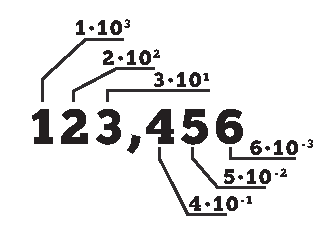
\includegraphics{pictures/Kuva5-1-desimaali-potenssit.pdf}
\end{center}
}

%Kymmenjärjestelmä saa nimensä siitä, että jokainen luvussa esiintyvä %numero kertoo sen paikkaa vastaavien kymmenen potenssien määrän.

\subsubsection*{Murtoluvun muuttaminen desimaaliluvuksi}

Murtoluku on tapa merkitä jakolaskua. Jakolaskun tuloksen esittämiseksi desimaalilukuna
käytetään peruskoulun alaluokilla opetettavaa jakokulmaa. Jakokulman ajatus on yksinkertaisesti kokeilla, kuinka monta jakajaa, sen kymmenesosaa, sadasosaa ja niin
edelleen jaettavaan mahtuu. Jakokulmat voi laskea käsin, laskin tekee saman nopeammin.

\begin{esimerkki}
Muutetaan $\frac{21}{4}$ desimaaliluvuksi laskemalla jakolasku $21 : 4$ jakokulmassa.

\[ 
\begin{array}{cccccc}
 & \underline{ \ \ } & \underline{5}, & \underline{2} & \underline{5} \\
 4 & \!\!|\,2 & 1, & 0 & 0 \\
 \underline{-} & \underline{2}& \underline{0} \\
 & & 1 &0 \\
 & \underline{-} &\underline{ \ \ }  & \underline{8} \\
 & & & 2 & 0 \\
 & & \underline{-} & \underline{2} & \underline{0} \\
 & &  & & 0
\end{array}
\]
Siis $\dfrac{21}{4} = 5,25$.
\end{esimerkki}

Vastaavasti laskien saadaan $\dfrac{3}{11}=0,272727\ldots \ $ :
\[ 
\begin{array}{cccccc}
 & \underline{ 0}, & \underline{2} & \underline{7} & \underline{2} & 
 \underline{\ldots} \\
 11 & \!\!|\,3, & 0 & 0 & 0 & \ldots \\
 \underline{-} & \underline{2}& \underline{2} \\
 & & \boldsymbol{8} &0 \\
 & \underline{-} &\underline{ 7 }  & \underline{7} \\
 & & & \boldsymbol{3} & 0 \\
 & & \underline{-} & \underline{2} & \underline{2} \\
 & &  & & \boldsymbol{8} & 0 \\
 & & & & & \ddots
\end{array}
\]
Koska jakojäännökset 3 ja 8 toistuvat loputtomiin, tämä desimaaliluku
ei ole päättyvä. Siinä on \emph{jakso}: numerosarja 27 toistuu.
Jaksoa voidaan merkitä yläviivan avulla seuraavasti:
\[ 0,27272727\ldots = 0,\overline{27}. \]

{\bf Kaikkien murtolukujen desimaaliesitykset ovat joko päättyviä tai jaksollisia.}
Vähennyslaskuissa syntyvät jakojäännökset ovat nimittäin aina jakajaa pienempiä, ja siksi
ne alkavat väistämättä toistaa itseään, ellei jako jossakin vaiheessa mene tasan.
Koska eri vaihtoehtoja jakojäännöksiksi on yksi jakajaa vähemmän,
jakson pituus on suurimmillaan yhden verran jakajaa pienempi. Esimerkiksi luvulla
$\dfrac{1}{7}=0,\overline{142857}$ jakso on pisin mahdollinen, $7-1=6$ numeron mittainen.

\laatikko{
Tässä on joitain murtolukujen desimaaliesityksiä, jotka on hyvä osata
\begin{alakohdat}
	\alakohta{$ \frac{1}{10} = 0,1$}
	\alakohta{$ \frac{1}{100} = 0,01$}
	\alakohta{$ \frac{1}{2} = 0,5$}
	\alakohta{$ \frac{1}{4} = 0,25$}
	\alakohta{$ \frac{3}{4} = 0,75$}
\end{alakohdat}
}

\subsubsection*{Desimaaliluvun muuttaminen murtoluvuksi}

\paragraph*{Päättyvät desimaaliluvut}

Päättyvät desimaaliluvut voidaan muuttaa murtoluvuiksi muuttamalla kukin
desimaali erikseen murtoluvuksi ja laskemalla syntyneet luvut yhteen.

\begin{esimerkki}
$21,37 = 21+ \frac{3}{10}+\frac{7}{100} =
\frac{2100}{100}+\frac{30}{100}+\frac{7}{100}
 = \frac{2100+30+7}{100} = \frac{2137}{100}.$
\end{esimerkki}

Tämä on turhan työlästä, ja paljon helpommalla päästäänkin kun lavennetaan luku ''niin monella kympillä, kuin siinä on numeroita desimaalipilkun jälkeen''. Täsmällisemmin sanottuna luvulla $10^n$, jossa $n$ on pilkun jälkeen tulevien numeroiden määrä.

\begin{esimerkki}
$21,47 = 21,37 \cdot  \frac{100}{100} = \frac{21,37 \cdot 100}{100} = \frac{2137}{100}$
\end{esimerkki}

%\begin{esimerkki}
%$0,007 = 0,007 \cdot 1 = 0,007 \cdot \frac{10^3}{10^3} = \frac{0,007 \cdot 1000}{1000} = %\frac{7}{1000}$
%\end{esimerkki}

%Menetelmän toimivuus kaikkien desimaalilukujen tapauksessa voidaan todistaa %tarkastelemalla desimaaliluvun määritelmää, mutta jätetään tässä tekemättä.

\paragraph*{Jaksolliset desimaaliluvut}

Minkä tahansa jaksollisen desimaaliluvun voi muuttaa murtoluvuksi seuraavalla tempulla.
Muutetaan esimerkiksi $0,575757\ldots$ murtoluvuksi. Jos merkitään
\[
\begin{array}{rcll}
x &=& \ \, 0,575757 \ldots\ , &\textrm{saadaan sadalla kertomalla} \\
100x &=& 57,575757 \ldots \ , &\textrm{joiden erotuksena} \\
100x - x &=& 57,57 \ldots - 0,57 \ldots \ , & \textrm{eli} \\
99x &=& 57, & \textrm{josta saadaan} \\
x &=& \frac{57}{99} = \frac{19}{33}.
\end{array}
\]
Siis $0,575757\ldots = \frac{19}{33}$. Menetelmä toimii kaikille jaksollisille
desimaaliluvuille: kerrotaan vain sopivalla luvun 10 potenssilla, jotta jakso
katoaa vähennyslaskussa.

\laatikko{
Nämä kannattaa muistaa:
\begin{alakohdat}
	\alakohta{$ \frac{1}{3} = 0,3333 \ldots$}
	\alakohta{$ \frac{2}{3} = 0,6666 \ldots$}
\end{alakohdat}
}

\begin{tehtavasivu}

\begin{tehtava}
Laske ja totea murtolukujen 
 $ \frac{1}{10} = 0,1$ , 
$ \frac{1}{100} = 0,01$ , 
 $ \frac{1}{2} = 0,5$ , 
$ \frac{1}{4} = 0,25$ , 
$ \frac{3}{4} = 0,75$
desimaaliesitysten paikkansapitävyys.
\end{tehtava}

\begin{tehtava}
Muuta murtoluvuksi.
%selkeys voitti täsmällisyyden ei siis murtolukumuotoon
	\begin{alakohdat}
		\alakohta{$43{,}532$}
		\alakohta{$5{,}031$}
		\alakohta{$0{,}23$}
		\alakohta{$0{,}3002$}
		\alakohta{$0{,}101$}
	\end{alakohdat}
\begin{vastaus}
	\begin{alakohdat}
		\alakohta{$ \frac{43532}{1000}$}
		\alakohta{$ \frac{5031}{1000}$}
		\alakohta{$ \frac{23}{100}$}
		\alakohta{$ \frac{3002}{1000}$}
		\alakohta{$ \frac{101}{1000}$}
	\end{alakohdat}
\end{vastaus}
\end{tehtava}

\begin{tehtava}%sovteht tai vaikea tehtävä? sivevennyksen takia
Muuta murtoluvuksi ja sievennä.
%selkeys voitti täsmällisyyden ei siis murtolukumuotoon
	\begin{alakohdat}
		\alakohta{$0{,}01$}
		\alakohta{$0{,}0245$}
		\alakohta{$0{,}004$}
		\alakohta{$0{,}001004$}
	\end{alakohdat}
\begin{vastaus}
	\begin{alakohdat}
		\alakohta{$ \frac{1}{100}$}
		\alakohta{$ \frac{49}{200}$}
		\alakohta{$ \frac{1}{250}$}
		\alakohta{$ \frac{251}{250~000}$}
	\end{alakohdat}
\end{vastaus}
\end{tehtava}

\begin{tehtava}
Muuta murtoluvuksi.
	\begin{alakohdat}
		\alakohta{$0,77777\ldots$}
		\alakohta{$0,151515 \ldots$}
		\alakohta{$2,05\overline{631}$}
		\alakohta{$0,99999\ldots$}
	\end{alakohdat}
\begin{vastaus}
	\begin{alakohdat}
		\alakohta{$\frac{7}{9}$ }
		\alakohta{$\frac{15}{99}=\frac{5}{33}$}
		\alakohta{$\frac{205\ 426}{99\ 900} = \frac{102\ 713}{49\ 950}$}
		\alakohta{$\frac{9}{9} = 1$}
	\end{alakohdat}
\end{vastaus}
\end{tehtava}

\begin{tehtava}
Muuta desimaaliluvuksi.
	\begin{alakohdat}
		\alakohta{$\frac{151}{250}$}
		\alakohta{$\frac{251}{625}$}
		\alakohta{$\frac{386}{1\ 250}$}
		\alakohta{$\frac{493}{500}$}
	\end{alakohdat}
\begin{vastaus}
	\begin{alakohdat}
		\alakohta{$0,604$}
		\alakohta{$0,4016$}
		\alakohta{$0,3088$}
		\alakohta{$0,986$}
	\end{alakohdat}
\end{vastaus}
\end{tehtava}

\begin{tehtava}
Muuta desimaaliluvuksi.
	\begin{alakohdat}
		\alakohta{$\frac{42}{11}$}
		\alakohta{$\frac{37}{13}$}
		\alakohta{$\frac{38}{99}$}
		\alakohta{$\frac{14}{15}$}
	\end{alakohdat}
\begin{vastaus}
	\begin{alakohdat}
		\alakohta{$3,\overline{81}$}
		\alakohta{$2,\overline{846153}$}
		\alakohta{$0,\overline{38}$}
		\alakohta{$0,9\overline{3}$}
	\end{alakohdat}
\end{vastaus}
\end{tehtava}

\begin{tehtava}
	Tunnissa on 60 sekuntia ja minuutissa on 60 sekuntia. Muuta seuraavat ajat tunneiksi.
	\begin{alakohdat}
		\alakohta{73 minuuttia}
		\alakohta{649 sekuntia}
		\alakohta{15 minuuttia ja 50 sekuntia}
		\alakohta{42 minuuttia ja 54 sekuntia}
	\end{alakohdat}
	\begin{vastaus}
		\begin{alakohdat}
			\alakohta{1,21666... tuntia}
			\alakohta{0,1802777... tuntia}
			\alakohta{0,263888... tuntia}
			\alakohta{0,715 tuntia}
		\end{alakohdat}
	\end{vastaus}
\end{tehtava}

\end{tehtavasivu}

\laatikko{
Joissain yhteyksissä käytetään muitakin \emph{lukujärjestelmiä} kuin kymmenjärjestelmää. Esimerkiksi tietokoneet käyttävät kaksikantajärjestelmää eli \emph{binäärijärjestelmää}. Binäärijärjestelmässä jokainen luvun numero kertoo sen paikkaa vastaavan kakkosen potenssien määrän kymmenen potenssien sijasta.

Binäärijärjestelmässä esitetty luku merkitään yleensä kirjoittamalla pieni kakkonen luvun jälkeen, esim. $10,01_2$.
}

\begin{esimerkki}
$10,01_2 = 1 \cdot 2^1 + 0 \cdot 2^0 + 0 \cdot 2^{-1} + 1 \cdot 2^{-2} = 2,25_{10}$
\end{esimerkki}

\begin{tehtavasivu}

\begin{tehtava}
Muunna seuraavat binääriluvut kymmenjärjestelmään.
	\begin{alakohdat}
		\alakohta{$101,0_2$}
		\alakohta{$1,00101_2$}
		\alakohta{$100101,1101_2$}
	\end{alakohdat}
\begin{vastaus}
	\begin{alakohdat}
		\alakohta{$5,0_{10}$}
		\alakohta{$1,15625_{10}$}
		\alakohta{$37.8125_{10}$}
	\end{alakohdat}
\end{vastaus}
\end{tehtava}

\begin{tehtava}
Muunna seuraavat luvut binäärijärjestelmään.
	\begin{alakohdat}
		\alakohta{$7,0_{10}$}
		\alakohta{$2,5_{10}$}
		\alakohta{$11,1875_{10}$}
	\end{alakohdat}
\begin{vastaus}
	\begin{alakohdat}
		\alakohta{$111,0_2$}
		\alakohta{$10,1_2$}
		\alakohta{$1011,0011_2$}
	\end{alakohdat}
\end{vastaus}
\end{tehtava}

\end{tehtavasivu}

    \section{Reaaliluvut}

Kaikki käyttämämme luvut eivät ole rationaalilukuja. Esimerkiksi $\sqrt{2}$ ei ole esitettävissä murtolukuna. Se tulee kuitenkin vastaan esimerksi suorakulmaisessa kolmiossa, jonka kateetit ovat pituudeltaan 1.

\laatikko{ TÄHÄN KUVA suorakulmaisesta kolmiosta, jonka sivut ovat
$1$, $1$ ja $\sqrt{2}$}

Luku $\sqrt{2}$ on \termi{irrationaaliluku}{irrationaaliluku}. Toinen tuttu peruskoulusta tuttu irrationaaliluku on ympyrän kehän pituuden suhde halkaisijaan: $\pi$. Irrationaaliluvut voidaan sijoittaa
lukusuoralle rationaalilukujen tapaan.

\begin{kuva}
lukusuora.pohja(1.3, 3.3, 11)
for i in range(13, 34):
	lukusuora.kohta(i / 10., "\\footnotesize " + str(i // 10) + "," + str(i % 10), nimi_ylos = False)
with vari("red"):
	lukusuora.kohta(pi, r"$\pi$")
	lukusuora.kohta(sqrt(2), r"$\sqrt{2}$")
\end{kuva}



Rationaalilukuja ja irrationaalilukuja kutsutaan yhdessä \emph{reaaliluvuiksi}. Reaalilukujen joukkoja merkitään $\R$.
Havainnollisesti reaalilukujen joukko sisältää kaikki lukusuoran luvut.

Rationaaliluvut eivät täytä koko koko reaalilukusuoraa, mutta niitä on niin tiheässä, että jokaisen kahden eri reaaliluvun välissä on rationaalilukuja. Jokaiselle irrationaaliluvulle voidaan löytää mielivaltaisen lähellä olevia rationaalilukuarvioita. Tätä kutsutaan irrationaalilukujen approksimoinniksi rationaaliluvuilla. Esimerkiksi lukua $\pi$ voidaan halutusta tarkkuudesta riippuen approksimoida rationaaliluvuilla
\[
3; \quad 3,1; \quad 3,14; \quad 3,142; \quad 3,1416; \quad 3,14159; \quad 3,141593; \quad \ldots 
\]

tai lukua $\sqrt{2}$ rationaaliluvuilla
\[
1; \quad \frac{3}{2}; \quad \frac{5}{4}; \quad \frac{11}{8}; \quad \frac{23}{16}; \quad \frac{45}{32}; \quad \ldots 
\]

\begin{kuva}
lukusuora.pohja(1, 1.5, 11)
lukusuora.kohta(1, r"\footnotesize $1$", nimi_ylos = False)
lukusuora.kohta(3./2, r"\footnotesize $\frac{3}{2}$", nimi_ylos = False)
lukusuora.kohta(5./4, r"\footnotesize $\frac{5}{4}$", nimi_ylos = False)
lukusuora.kohta(11./8, r"\footnotesize $\frac{11}{8}$", nimi_ylos = False)
lukusuora.kohta(23./16, r"\footnotesize $\frac{23}{16}$", nimi_ylos = False)
lukusuora.kohta(45./32, r"\footnotesize $\frac{45}{32}$", nimi_ylos = False)
with vari("red"):
	lukusuora.kohta(sqrt(2), r"$\sqrt{2}$")
\end{kuva}

\laatikko{
Kaikki rationaalilukuja koskevat laskusäännöt pätevät myös reaaliluvuille.
}

Väite on uskottava, sillä reaalilukuja voi aina approksimoida mielivaltaisen tarkasti rationaaliluvuilla. Väitteen tarkempi perusteleminen ei tämän kurssin työkaluilla vielä onnistu.

Siinä missä rationaalilukujen desimaaliesitykset ovat päättyviä tai jaksollisia, ovat irrationaalilukujen desimaaliesitykset päättymättömiä ja
jaksottomia. Monissa tapauksissa on hyvin vaikeaa osoittaa luku irrationaaliseksi. Tällöin vaaditaan keinoja, jotka eivät kuulu tämän kurssin laajuuteen.

Luvun
\[\sqrt{2} \approx 1,414213562373095048801688724209\ldots\]
desimaaliesityksessä on kyllä toistuvia kohtia, esimerkiksi numeropari $88$ esiintyy kahdesti. Siinä ei kuitenkaan ole jaksoa, jonka luvut toistuisivat yhä uudestaan
samassa järjestyksessä, kuten luvussa $3,80612312312312\ldots$.

Reaalilukujen ominaisuuksista kerrotaan lisää liitteessä \ref{aksioomat}.


Reaalilukujen myötä kaikki lukiokursseissa esiintyvät lukujoukot on nyt esitelty. Ne on lueteltu seuraavassa:
\begin{center}\begin{tabular}{l|c|l}
Joukko & Symboli & Mitä ne ovat\\
\hline
Luonnolliset luvut & $\N$ &
Luvut $0$, $1$, $2$, $3$, $\ldots$ \\
Kokonaisluvut & $\Z$ & Luvut $\ldots$ $-2$, $-1$, $0$, $1$, $2$ $\ldots$ \\ 
Rationaaliluvut & $\Q$ & Luvut, jotka voidaan esittää
murtolukuna \\
Reaaliluvut & $\R$ & Kaikki lukusuoran luvut \\
& & eli kaikki desimaaliluvut
\end{tabular} \end{center} 

\begin{tikzpicture}[line cap=round,line join=round,>=triangle 45,x=0.5cm,y=0.5cm]
\clip(-7.4,-8.8) rectangle (16.8,8.6);
\draw [rotate around={0.5:(2.2,0)}] (2.2,0) ellipse (1.1cm and 0.9cm);
\draw [rotate around={-0.8:(2.5,0)}] (2.5,0) ellipse (2cm and 1.6cm);
\draw [rotate around={-0.8:(2.5,0)}] (2.5,0) ellipse (2.9cm and 2.6cm);
\draw (2,1.5) node[anchor=north west] {$\N$};
\draw (4.0,2.7) node[anchor=north west] {$\Z$};
\draw (5.5,3.9) node[anchor=north west] {$\Q$};
%\draw (6.6,-4.6) node[anchor=north west] {{\scriptsize Irrationaaliluvut}};
\draw (9.5,6.4) node[anchor=north west] {$\R$};
\draw [rotate around={0.5:(4.4,0)}] (4.4,0) ellipse (5cm and 4.2cm);
%\draw [rotate around={18.2:(7.9,-5.4)}] (7.9,-5.4) ellipse (2.7cm and 0.6cm);
\draw (0.8,1.6) node[anchor=north west] {$1$};
\draw (1,-0.4) node[anchor=north west] {$5$};
\draw (2.4,-0.2) node[anchor=north west] {$101$};
\draw (4.8,0.7) node[anchor=north west] {$-5$};
\draw (1.2,-1.7) node[anchor=north west] {$0$};
\draw (1.2,3.1) node[anchor=north west] {$-14$};
%\draw (4.1,-1) node[anchor=north west] {$75$};
\draw (4.2,-2.8) node[anchor=north west] {$-\frac{1}{3}$};
\draw (6.6,1.4) node[anchor=north west] {$2\frac{1}{2}$};
\draw (-1.6,0.9) node[anchor=north west] {$-3$};
%\draw (0.4,-3.1) node[anchor=north west] {$-4$};
\draw (2.4,4.7) node[anchor=north west] {$2,6$};
\draw (-1.3,4.1) node[anchor=north west] {$\frac{5}{7}$};
\draw (-2.7,-1) node[anchor=north west] {$0,1$};
\draw (5.5,-5.9) node[anchor=north west] {$\pi$};
\draw (9.1,-3) node[anchor=north west] {$\sqrt[]{2}$};
%\draw (6,-4.7) node[anchor=north west] {$-\frac{\pi}{2}$};
%\draw (9.8,1.6) node[anchor=north west] {$\frac{5}{2}$};
\draw (10.5,3) node[anchor=north west] {$\frac{1}{\sqrt{2}}$};
%\draw (4.4,7.3) node[anchor=north west] {$3$};
\draw (-0.1,-5.3) node[anchor=north west] {$\sqrt{15}$};
%\draw (-4.9,1.5) node[anchor=north west] {$-5$};
\draw (11.8,-0.9) node[anchor=north west] {$-\frac{\pi}{2}$};
\draw (-0.6,6.8) node[anchor=north west] {$0,10110111011110\ldots$};
%\draw (-3.7,-3) node[anchor=north west] {$-3$};
\end{tikzpicture}

Lukualueita voidaan laajentaa lisää vielä tästäkin, esimerkiksi \emph{kompleksiluvuiksi}, jotka voidaan esittää tason pisteinä. Kompleksilukuja tarvitaan muun muassa insinöörialoilla yliopistoissa ja ammattikorkeakouluissa. Esimerkiksi vaihtosähköpiirien analyysissä, signaalinkäsittelyssä ja säätötekniikassa käytetään runsaasti kompleksilukuja. Kompleksiluvut ovat tärkeitä myös matematiikan tutkimuksessa itsessään.

\subsection*{Harjoitustehtäviä}

\begin{tehtava}
Ovatko seuraavat luvut rationaalilukuja vai irrationaalilukuja? Kunkin desimaalit
noudattavat yksinkertaista sääntöä.
\begin{alakohdat}
\alakohta{$0,123456789101112131415 \ldots$}
\alakohta{$2,415115115115115115115 \ldots$}
\alakohta{$1,010010001000010000010 \ldots$}
\end{alakohdat}
\begin{vastaus}
a) irrationaaliluku \ b) rationaaliluku (jakso on 151) \ c) irrationaaliluku
\end{vastaus}
\end{tehtava}

\begin{tehtava}
Mikä on pienin lukua -3 suurempi luku \\
a) kokonaislukujen \ b) luonnollisten lukujen \ c) reaalilukujen joukossa?
\begin{vastaus}
a) -2 \ b) 0 \ c) Sellaista ei ole. Jos nimittäin $a > -3$, niin keskiarvo
$\frac{-3+a}{2}$ on vielä lähempänä lukua $-3$. 
\end{vastaus}
\end{tehtava}

\begin{tehtava}
$\boldsymbol{[\star]}$ Osoita, että \\
a) jokaisen kahden rationaaliluvun välissä on rationaaliluku \\
b) jokaisen kahden rationaaliluvun välillä on irrationaaliluku \\
c) jokaisen kahden irrationaaliluvun välissä on rationaaliluku \\
d) jokaisen kahden irrationaaliluvun välissä on irrationaaliluku. \\
e) Perustele edellisten kohtien avulla, että minkä tahansa kahden luvun
välissä on äärettömän monta rationaali- ja irrationaalilukua.
\begin{vastaus}
Vihjeet: a) keskiarvo \ b) $\sqrt{2}$ on irrationaaliluku. Käytä
painotettua keskiarvoa. \ c) pyöristäminen \ d) hyödynnä b-kohtaa
e) keskiarvot
\end{vastaus}
\end{tehtava}

    \section{Juuret}

\subsection*{Neliöjuuri}

Ajatellaan, että neliön pinta-ala on $a$. Halutaan tietää, mikä on kyseisen neliön sivun pituus. Vastausta tähän kysymykseen kutsutaan luvun $a\ge 0$ neliöjuureksi ja merkitään $\sqrt{a}$. Luvun $a$ neliöjuuri on myös yhtälön $x^2 = a$ ratkaisu. Tällöin täytyy kuitenkin huomata, että myös luku $x=-\sqrt{a}$ toteuttaa kyseisen yhtälön. Neliöjuurella tarkoitetaan kyseisen yhtälön epänegatiivista ratkaisua. Tämä on luonnollista, koska neliön sivun pituus ei voi olla negatiivinen luku.

\laatikko{Luvun $a$ neliöjuuri on epänegatiivinen luku, jonka neliö on $a$. Tämä voidaan ilmaista myös $(\sqrt{a})^2=a$.}

Neliöjuurta ei tällä kurssilla määritellä negatiivisille luvuille, koska neliön pinta-ala on aina positiivinen luku tai nolla. Käytännössä lukujen neliöjuuria lasketaan usein laskimella.


\begin{esimerkki}
Laske.
\begin{alakohdat}
\alakohta{$\sqrt{4}$}

\alakohta{$\sqrt{144}$}

\alakohta{$\sqrt{4471}$.}
\end{alakohdat}

{\bf Ratkaisut.}

a)
Laskimella tai päässä laskemalla saadaan, että $\sqrt{4} = 2$, koska $2\geq0$ ja $2^2 =4$.

b) 
$\sqrt{144}=12$. Tämä voidaan vielä tarkistaa laskemalla $12^2 = 12\cdot 12=144$.

c)
$\sqrt{4471}\approx 66,9$. Vertailun vuoksi laskimella saadaan myös $67\cdot 67=4489$.

{\bf Vastaukset.}
a) $2$, b) $12$, c) $66,9$.

\end{esimerkki}

\begin{esimerkki}
Taulutelevision kooksi (lävistäjäksi) on ilmoitettu mainoksessa $46,0$ tuumaa ($116,8$ cm) ja kuvasuhteeksi 16:9. Kuinka leveä televisio on (senttimetreinä)?

{\bf Ratkaisu.}

Taulutelevision halkaisija, alareuna ja toinen sivu muodostavat suorakulmaisen kolmion. Kolmion hypotenuusa on television halkaisija ja kateetit alareuna ja toinen sivu.

Kuvasuhteen perusteella kateettien pituuksia voidaan merkitä $16x$ ja $9x$. Pythagoraan lauseesta saadaan
\[
(116,8)^2 = (16x)^2 + (9x)^2
\]
eli
\[
13642,24 = (256+81)x^2.
\]
Siten
\[
x^2 = \frac{13642,24}{337}
\]
ja siis
\[
x= \sqrt{\frac{13642,24}{337}} \approx 6,36.
\]
Television leveys on noin $16x = 16\cdot 6,36\approx 102$ cm.

{\bf Vastaus.} Noin $102$ cm.
\end{esimerkki}



\subsection*{Kuutiojuuri}

Kuution tilavuus on $a$. Halutaan tietää, mikä on kyseisen kuution sivun pituus. Vastausta tähän kysymykseen kutsutaan luvun $a\ge 0$ kuutiojuureksi ja merkitään $\sqrt[3]{a}$. Luvun $a$ kuutiojuuri on myös yhtälön $x^3 = a$ vastaus.

\laatikko{Luvun $a$ kuutiojuuri on luku, jonka kuutio on $a$. Tämä voidaan ilmaista myös $(\sqrt[3]{a})^3=a$.}

Jos $a<0$, niin kysymys kuutiosta jonka tilavuus on $a$, ei ole mielekäs. Tästä huolimatta kuutiojuuri määritellään myös negatiivisille luvuille. Syy tähän on, että yhtälöllä $x^3=a$ on tässäkin tapauksessa yksikäsitteinen ratkaisu. Positiivisen luvun kuutiojuuri on aina positiivinen ja negatiivisen luvun kuutiojuuri on aina negatiivinen luku. Kuutiojuuren voi siis ottaa mistä tahansa reaaliluvusta.


\begin{esimerkki}
Laske.
\begin{alakohdat}
\alakohta{$\sqrt[3]{27}$}

\alakohta{$\sqrt[3]{1397}$}

\alakohta{$\sqrt[3]{2197}$.}
\end{alakohdat}

{\bf Ratkaisut.}

a)
Laskimella tai päässä laskemalla saadaan, että $\sqrt[3]{27} = 3$, koska  $3^3 =3\cdot 3\cdot 3=27$.

b) 
$\sqrt[3]{1397}\approx 11,18$. 

c)
$\sqrt[3]{2197}=13$.
Tämä voidaan vielä tarkistaa laskemalla $13^3 = 13\cdot 13\cdot 13=2197$.

{\bf Vastaukset.}

a) $3$, b) $11,18$, c) $13$.
\end{esimerkki}


\subsection*{Korkeammat juuret}


Yhtälön $x^n=a$ ratkaisujen avulla voidaan määritellä $n$:s juuri mille tahansa positiiviselle kokonaisluvulle $n$. Neliö- ja kuutiojuurten tapauksesta voidaan kuitenkin voi huomata, että kuutiojuuri on määritelty kaikille luvuille, mutta neliöjuuri vain epänegatiivisille luvuille. Tämä toistuu myös muissa juurissa: parilliset ja parittomat juuret on määriteltävä erikseen.

Juurimerkinnällä $\sqrt[n]{a}$ (luetaan \emph{$n$:s juuri} luvusta $a$) tarkoitetaan lukua, joka toteuttaa ehdon $(\sqrt[n]{a})^n = a$. Jotta juuri olisi yksikäsitteisesti määritelty, asetetaan lisäksi, että parillisessa tapauksessa $n$:s juuri tarkoittaa kyseisen yhtälön epänegatiivista ratkaisua.
%($\sqrt{a}, \sqrt[4]{a}, \sqrt[6]{a}$\ldots) vaadittava, että $b\ge0$.



\laatikko{
{\bf Parillinen juuri}

Kun $n$ on parillinen luku, luvun $a \ge 0$ $n$:s juuri on luku $b \ge 0$, jonka $n$:s potenssi on $a$, eli $b^n = a$. Lukua $b$ merkitään $\sqrt[n]{a}$, eli $\left(\sqrt[n]{a}\right)^n = a$. Edelleen, kun $n$ on parillinen luku, $n$:ttä juurta ei ole määritelty negatiivisille luvuille.
}

Luvun toista juurta, eli neliöjuurta $\sqrt[2]{a}$ merkitään yleensä yksinkertaisemmin $\sqrt{a}$.

\laatikko{
{\bf Pariton juuri}

Kun $n$ on pariton luku, luvun $a \in \R$ $n$:s juuri on yksikäsitteinen luku $b \in \R$, jonka $n$:s potenssi on $a$, eli $b^n = a$. Lukua $b$ merkitään $\sqrt[n]{a}$, eli $\left(\sqrt[n]{a}\right)^n = a$. Erityisesti $n$:s juuri on määritelty parittomilla $n$ myös negatiivisille luvuille toisin kuin $n$:s juuri parillisilla $n$.
}

Korkeampien juurten laskeminen tapahtuu tavallisesti laskimella.

\begin{esimerkki}
Laske.
\begin{alakohdat}
\alakohta{$\sqrt[4]{256}$}
\alakohta{$\sqrt[5]{-243}$}
\alakohta{$\sqrt[4]{-8}$}
\end{alakohdat}

{\bf Ratkaisut.}

a) Laskimella saadaan $\sqrt[4]{256}=4$, koska $4^4=256$.

b) Laskimella $\sqrt[5]{-243}=-3$, koska $(-3)^5=-243$.

c) Luvun $-8$ neljäs juuri $\sqrt[4]{-8}$ ei ole määritelty, koska minkään luvun neljäs potenssi ei ole negatiivinen.
\end{esimerkki}

\begin{tehtavasivu}

%Antti, lisää tämä
\begin{tehtava}
Laske seuraavat neliöjuuret laskimella.\\
a) $\sqrt{320}$,\ b) $\sqrt{15}$,\ c) $\sqrt{71}$
\begin{vastaus}
a) $17{,}89$ b) $3{,}87$ c) $8{,}43$
\end{vastaus}
\end{tehtava}


\begin{tehtava}
Laske $\sqrt{8100}$ päässä ajattelemalla juurrettava luku sopivana tulona.
\begin{vastaus}
$\sqrt{8100}=\sqrt{81}\sqrt{100}=9\cdot 10$.
\end{vastaus}
\end{tehtava}


\begin{tehtava}
Etsi luku $a>0$ jolle $a^4=83521$.
\begin{vastaus}
$a=\sqrt{\sqrt{83521}}$.
\end{vastaus}
\end{tehtava}


\begin{tehtava}
Oletetaan että suorakaiteen leveyden suhde korkeuteen on $2$ ja suorakaiteen pinta-ala on $10$. Mikä on suorakaiteen 
leveys ja korkeus?
\begin{vastaus}
Suorakaide muodostuu kahdesta vierekkäisestä neliöstä, joiden pinta-ala on $5$. Tämän neliön sivun pituus on $\sqrt{5}$.
Siis suorakaiteen korkeus on $\sqrt{5}$ ja leveys $2\sqrt{5}$.
\end{vastaus}
\end{tehtava}


\begin{tehtava}
Ajatellaan suorakulmaista hiekkakenttää, jonka pinta-ala on 1 aari ($100~\mathrm{m}^2$). Lyhyemmän ja pidemmän sivujen 
pituuksien suhde on 4:3. Laske Pythagoraan lauseen avulla matka hiekkakentän kulmasta kauimmaisena olevaan kulmaan.
\begin{vastaus}
$\frac{4}{3}x^2=100$ joten $x = \sqrt{\frac{300}{4}}$. 
Hypotenuusa: $\sqrt{x^2 + (\frac{4}{3}x)^2}=\sqrt{\frac{300}{4}+\frac{16}{9}\cdot \frac{300}{4}}
=\frac{5}{3}\sqrt{\frac{300}{4}}\approx 14{,}4$.
\end{vastaus}
\end{tehtava}


\begin{tehtava}
Laske.
a) $\sqrt{64}$ \quad b) $\sqrt{-64}$ \quad c) $\sqrt[3]{64}$ \quad d) $\sqrt[3]{-64}$

\begin{vastaus}
a) 8 b) Ei määritelty c) 4 d) -4
\end{vastaus}
\end{tehtava}

\begin{tehtava}
Laske.
a) $\sqrt[4]{81}$ \quad b) $\sqrt[4]{-81}$ \quad c) $\sqrt[5]{32}$ \quad d) $\sqrt[5]{-32}$

\begin{vastaus}
a) 3 b) Ei määritelty c) 2 d) -2
\end{vastaus}
\end{tehtava}

\begin{tehtava}
Laske luvun $10$ potensseja: $10^1, 10^2, 10^3, 10^4, \ldots$ Kuinka monta nollaa on luvussa $10^n$? Laske sitten $\sqrt[6]{1~000~000}$ ja $\sqrt[10]{10~000~000~000}$.

\begin{vastaus}
$10^1 = 10, 10^2 = 100, 10^3 = 1~000, 10^4 = 10~000$. Luvussa $10^n$ on $n$ kappaletta nollia. Niinpä $\sqrt[6]{1~000~000} = 10$ ja $\sqrt[10]{10~000~000~000} = 10$.
\end{vastaus}
\end{tehtava}

\begin{tehtava}
Onko annettu juuri määritelty kaikilla luvuilla $a$? Millaisia arvoja juuri voi saada luvusta $a$ riippuen?\\
a) $\sqrt[4]{a^2}$ \quad b) $\sqrt[4]{-a^2}$ \quad c) $\sqrt[4]{(-a)^2}$ \quad d) $- \sqrt[4]{a^2}$

\begin{vastaus}

\begin{alakohdat}
	\alakohta{Juuri on määritelty kaikilla luvuilla $a$, koska kaikkien lukujen neliöt ovat vähintään nolla. Vastaus on aina epänegatiivinen.}
	\alakohta{Juuri on määritelty vain luvulla $a = 0$. Muilla $a$:n arvoilla $-a^2$ on negatiivinen, jolloin parillinen juuri ei ole määritelty. Ainoa vastaus, joka voidaan saada, on siis $\sqrt[4]{0} = 0$.}
	\alakohta{Juuri on määritelty kaikilla luvuilla $a$, koska $(-a)^2$ on aina vähintään nolla. Vastaus on aina epänegatiivinen.}
	\alakohta{Juuri on määritelty kaikilla luvuilla $a$, koska kaikkien lukujen neliöt ovat vähintään nolla. Vastaus on aina ei-positiivinen, koska $\sqrt[4]{a^2}$ on aina epänegatiivinen.}
\end{alakohdat}
\end{vastaus}
\end{tehtava}

\begin{tehtava}
Onko annettu juuri määritelty kaikilla luvuilla $a$? Millaisia arvoja juuri voi saada luvusta $a$ riippuen?\\
a) $\sqrt[5]{a^2}$ \quad b) $\sqrt[5]{a^3}$ \quad c) $\sqrt[5]{-a^2}$ \quad d) $- \sqrt[5]{a^2}$

\begin{vastaus}

\begin{alakohdat}
	\alakohta{Juuri on määritelty kaikilla luvuilla $a$. Vastaus on aina epänegatiivinen.}
	\alakohta{Juuri on määritelty kaikilla luvuilla $a$. Vastaus voi olla mikä tahansa luku.}
	\alakohta{Juuri on määritelty kaikilla luvuilla $a$. Vastaus on aina ei-positiivinen.}
	\alakohta{Juuri on määritelty kaikilla luvuilla $a$. Vastaus on aina ei-positiivinen.}
\end{alakohdat}
\end{vastaus}
\end{tehtava}

\begin{tehtava}
Sievennä $(3+\sqrt{3}x)^4:(\sqrt{3}+x)^3$.
\begin{vastaus}
$3 + \sqrt{3}x$
\end{vastaus}
\end{tehtava}

\begin{tehtava}
(YO 1888 1) Mikä on a/b:n arvo, jos \\
$ (\sqrt{a}+\sqrt{b}):(\sqrt{a}-\sqrt{b})=\sqrt{2}$ ?
\begin{vastaus}
$(3-2\sqrt{2}):(3+2\sqrt{2})$
\end{vastaus}
\end{tehtava}

\end{tehtavasivu}

    \section{Murtopotenssi}

Seuraavaksi tutkitaan potenssin käsitteen laajentamista tilanteeseen, jossa eksponenttina on murtoluku.
Esimerkiksi voidaan pohtia, mitä tarkoittaa merkintä $2^\frac{1}{3}$? Potenssin laskusääntöjen perusteella
\[
(2^{m})^n = 2^{mn},\textrm{ kun }m,n\in \Z.
\]
Siten on luonnollista ajatella, että murtopotenssille $2^\frac{1}{3}$ pätee
\[
(2^\frac{1}{3})^3 = 2^\frac{3}{3} = 2^1=2.
\]
Koska luvun $2$ kuutiojuuri toteuttaa yhtälön $(\sqrt[3]{2})^3=2$, täytyy siis asettaa $2^\frac{1}{3}=\sqrt[3]{2}$. Yleisemmin asetetaan $a^\frac{1}{n} =\sqrt[n]{a}$, kun $n$ on positiivinen kokonaisluku ja $a\ge 0$.

Kaavan on edelleen luontevaa ajatella yleistyvän niin, että esimerkiksi
\[
(2^{\frac{1}{3}})^2 = 2^{\frac{2}{3}}.
\]
Yleisemmin otetaan murtopotenssin $a^\frac{m}{n}$ määritelmäksi
\[
a^\frac{m}{n} = (a^{\frac{1}{n}})^m = (\sqrt[n]{a})^m,
\]
kun $m$ ja $n$ ovat kokonaislukuja ja $n>0$. 

\laatikko{{\bf Murtopotenssimerkinnät}
\[
a^\frac{1}{n} = \sqrt[n]{a},\textrm{ kun }a\geq 0. 
\]
Erityisesti $a^\frac{1}{2}=\sqrt{a}$.
\[
a^\frac{m}{n} =  (\sqrt[n]{a})^m,\textrm{ kun }a > 0. % Issue 68 fiksattu.
\]
}

%\laatikko{Murtopotenssimerkintä: }

Kun murtolukueksponentit määritellään näin, kaikki aikaisemmat potenssien
laskusäännöt ovat sellaisenaan voimassa myös niille. Esimerkiksi kaavat
\[ a^q\cdot a^q = a^{p+q}, \quad (a^p)^q = a^{pq}, \quad (ab)^q=a^qb^q \]
pätevät kaikille rationaaliluvuille $p$ ja $q$.  Näiden kaavojen todistukset on esitetty liitteessä \ref{pot_todistukset}.

{\bf Huomautus määrittelyjoukosta}. Murtopotenssimerkintää käytettäessä vaaditaan, että $a\geq 0$ myös silloin, kun $n$ on pariton. Syy tähän on seuraava. Esimerkiksi $\sqrt[3]{-1}=-1$, koska $(-1)^3=-1$, mutta lauseketta $(-1)^\frac{1}{3}$ ei ole tällöin määritelty. Murtopotenssimerkinnän määrittelystä voi tällöin seurata yllättäviä ongelmia:
\[
 -1 = \sqrt[3]{-1} = (-1)^\frac{1}{3} = (-1)^\frac{2}{6}
= ((-1)^2)^\frac{1}{6} = 1^\frac{1}{6} = \sqrt[6]{1} = 1. 
\]
Luvun $\frac{1}{3}$ lavennus muotoon $\frac{2}{6}$ on ongelman ydin, mutta murtolukujen lavennussäännöistä luopuminen olisi myös hankalaa. Siksi sovitaan, ettei murtopotenssimerkintää käytetä, jos kantaluku on negatiivinen.

Nolla kantalukuna taas aiheuttaa ongelmia, jos eksponentti on negatiivinen. Esimerkiksi
\[
 0^{-\tfrac{1}{2}}=\frac{1}{0^\frac{1}{2}}=\frac{1}{0}, % Issue 68 fiksattu.
\]
jota ei ole määritelty.

\begin{esimerkki}
Muuta lausekkeet $\sqrt[5]{3}$ ja $(\sqrt[4]{a})^7$ murtopotenssimuotoon.

{\bf Ratkaisu.}

$\sqrt[5]{3} = 3^\frac{1}{5}$, \\
$(\sqrt[4]{a})^7 = (a^\frac{1}{4})^7=a^\frac{7}{4}$
\end{esimerkki}

\begin{esimerkki}
Sievennä lauseke $8^\frac{2}{3}$.

{\bf Ratkaisu.}
 $8^\frac{2}{3} = (\sqrt[3]{8})^2 = 2^2 = 4.$
\end{esimerkki}

\begin{tehtavasivu}

Muuta lausekkeet murtopotenssimuotoon.

\begin{tehtava}
	\begin{alakohdat}
		\alakohta{$\sqrt[3]{a}$} 
		\alakohta{$\sqrt[6]{a}$} 
	\alakohta{$\sqrt[n]{a}$}
	\end{alakohdat}
	\begin{vastaus}
		\begin{alakohdat}
			\alakohta{$a^\frac{1}{3}$} 
			\alakohta{$a^\frac{1}{6}$}
			\alakohta{$a^\frac{1}{n}$}
		\end{alakohdat}
	\end{vastaus}
\end{tehtava}

\begin{tehtava}
	\begin{alakohdat}
		\alakohta{$(\sqrt[3]{b})^6$}
		\alakohta{$(\sqrt[6]{b^3})$}
		\alakohta{$(\sqrt[5]{b})^2$}
		\alakohta{$(\sqrt[16]{\ddot{o}^4})$}
	\end{alakohdat}
	\begin{vastaus}
		\begin{alakohdat}
			\alakohta{$b^2$}
			\alakohta{$b^\frac{1}{2}$}
			\alakohta{$b^\frac{2}{5}$}
			\alakohta{$\ddot{o}^\frac{1}{4}$}
		\end{alakohdat}
	\end{vastaus}
\end{tehtava}

Sievennä.
\begin{tehtava}
	\begin{alakohdat}
		\alakohta{$x^\frac{1}{5}$}
		\alakohta{$x^\frac{4}{3}$}
		\alakohta{$x^\frac{8}{4}$}
		\alakohta{$x^\frac{25}{100}$}
\end{alakohdat}
	\begin{vastaus}
		\begin{alakohdat}	
			\alakohta{$(\sqrt[5]{x})$}
			\alakohta{$(\sqrt[3]{x})^4$}
			\alakohta{$x^2$}
			\alakohta{$(\sqrt[4]{x})$}
		\end{alakohdat} 
	\end{vastaus}
\end{tehtava}

\begin{tehtava}
	\begin{alakohdat}
		\alakohta{$9^\frac{1}{2}$}
		\alakohta{$8^\frac{1}{3}$}
		\alakohta{$4^\frac{3}{2}$}
		\alakohta{$81^\frac{3}{4}$}
	\end{alakohdat}
	\begin{vastaus}
		\begin{alakohdat}
			\alakohta{$3$}
			\alakohta{$2$}
			\alakohta{$8$}
			\alakohta{$27$} 
		\end{alakohdat}
	\end{vastaus}
\end{tehtava}

\begin{tehtava}
	\begin{alakohdat}
		\alakohta{$x^{-\frac{1}{3}}$} 
		\alakohta{$x^\frac{5}{-2}$}
		\alakohta{$x^{3 \frac{1}{2}}$}
		\alakohta{$x^{2 \frac{-4}{-7}}$}
	\end{alakohdat}
	\begin{vastaus}
		\begin{alakohdat}
			\alakohta{$\frac{1}{\sqrt[3]{x}}$} 
			\alakohta{$\frac{1}{\sqrt{x^5}}$} 
			\alakohta{$\sqrt{x^3}$} 
			\alakohta{$\sqrt[7]{x^8}$} 
		\end{alakohdat}
	\end{vastaus}
\end{tehtava}

\begin{tehtava}
	\begin{alakohdat}
		\alakohta{$4^\frac{3}{4}$}
		\alakohta{$2^\frac{5}{1}$} 
		\alakohta{$16^\frac{2}{3}$}
		\alakohta{$5^\frac{5}{3}$}
	\end{alakohdat}
	\begin{vastaus}
		\begin{alakohdat}
			\alakohta{$2\sqrt{2}$}
			\alakohta{$32$} 
			\alakohta{$(\sqrt[3]{16})^2$} 
			\alakohta{$5(\sqrt[3]{5})^2$} 
		\end{alakohdat}
	\end{vastaus}
\end{tehtava}

\begin{tehtava}
	\begin{alakohdat}
	$\boldsymbol{[\star]}$ Oletetaan, että $a\leq0$ \\
		\alakohta{$\frac{\sqrt[3]{a^2}-\sqrt[3]{a}}{\sqrt[3]{a}}$}
		\alakohta{$\sqrt{\frac{\sqrt{a}^2\sqrt[3]{a^6}}{4a}}$}
		\alakohta{$\sqrt[7]{\frac{a-\sqrt{a}^2}{a^0}}$} 
		\alakohta{$\sqrt{\sqrt{a^3}\left(\frac{a^7}{\sqrt[5]{a^3}}\right)^0\sqrt{\frac{a^5}{a^2}}}$}
	\end{alakohdat}
	\begin{vastaus}
		\begin{alakohdat}
			\alakohta{$\sqrt[3]{a}-1$} 
			\alakohta{$\frac{1}{2}a$} 
			\alakohta{$1$} 
			\alakohta{$a\sqrt{a}$}
		\end{alakohdat}
	\end{vastaus}
\end{tehtava}

Muuta murtopotenssimuotoon.

\begin{tehtava}
	\begin{alakohdat}
		\alakohta{$\sqrt{\sqrt{k}}$} 
		\alakohta{$\sqrt[3]{\sqrt[4]{k}}$}
		\alakohta{$\sqrt{m\sqrt{m}}$}
		\alakohta{$\sqrt[5]{m\sqrt[7]{m}}$}
	\end{alakohdat}
	\begin{vastaus}
		\begin{alakohdat}
			\alakohta{$k^\frac{1}{4}$} 
			\alakohta{$k^\frac{1}{12}$} 
			\alakohta{$m^\frac{3}{4}$} 
			\alakohta{$m^\frac{8}{35}$}
		\end{alakohdat}
	\end{vastaus}
\end{tehtava}

\begin{tehtava}
	\begin{alakohdat}
		\alakohta{$\sqrt[3]{\sqrt[3]{\alpha}^2}$} 
		\alakohta{$\sqrt[5]{q^2\sqrt{q}}$} 
		\alakohta{$\left(\sqrt{å^4\sqrt{å}}\right)^3$}
	\end{alakohdat}
	\begin{vastaus}
		\begin{alakohdat}
			\alakohta{$\alpha^\frac{2}{9}$}
			\alakohta{$q^\frac{1}{2}$} 
			\alakohta{$å^\frac{27}{4}$}
		\end{alakohdat}
	\end{vastaus}
\end{tehtava}
 
\begin{tehtava}
	\begin{alakohdat}
	$\boldsymbol{[\star]}$ Tutki laskimella, miten laskutoimitukset
	\[ x^x, \quad x^{x^x}, \quad x^{x^{x^x}}, \quad \ldots\]
	käyttäytyvät, kun eksponenttien määrää kasvatetaan mielivaltaisen
	suureksi.\\
		\alakohta{Tutki arvoja $x=1,3$, $x=1,7$ ja $x=0,05$.}
		\alakohta{Millä luvun $x$ positiivisilla arvoilla potenssitornien arvot}
			vakiintuvat tiettyyn lukuun?
	\end{alakohdat}
	\begin{vastaus}
		\begin{alakohdat}
			\alakohta{Kun $x = 1,3$, tornien arvot vakiintuvat lukuun $1,4709\ldots$;
				kun $x = 1,7$, tornien arvot kasvavat mielivaltaisen suuriksi;
				kun $x=0,05$, tornien arvot vuorottelevat lukujen $0,136\ldots$
				ja $0,664\ldots$ välillä.}
			\alakohta{Arvot vakiintuvat, kun $0,00659 \ldots \leq x \leq 1,444667\ldots$;
				tämän voi esittää muodossa $\frac{1}{e^e} \leq x \leq \sqrt[e]{e}$, missä
				$e$ on luku nimeltään Neperin luku. Desimaalilukuna $e = 2,718281828459 \ldots$ .}
		\end{alakohdat}
\end{vastaus}
\end{tehtava}
\begin{tehtava}
	$\boldsymbol{[\star]}$ Potenssitornissa $x^{x^{x^{x^{\mathstrut^{.^{.^{.}}}}}}} $
		on äärettömän monta päällekkäistä eksponenttia. Yhtälöllä
	$ x^{x^{x^{x^{\mathstrut^{.^{.^{.}}}}}}} =2$
		on yksi ratkaisu. Etsi se.
\begin{vastaus}
	$x = \sqrt{2}$
\end{vastaus}
\end{tehtava}
\end{tehtavasivu}


\chapter{Yhtälöt}
    \section{Yhtälö}

Monissa käytännön tilanteissa jokin suure voidaan päätellä tai laskea kahdella eri tavalla. Nämä tavat voidaan merkitä lukuina tai kirjoittaa lausekkeiksi. Merkitsemällä näin saadut lukuarvot ja lausekkeet yhtäsuuriksi saadaan \emph{yhtälö}. Yhtälö on siis kahden lausekkeen merkitty yhtäsuuruus. Yhtälöitä esiintyy usein käytännön tilanteissa.

\begin{esimerkki}
Merkitään lausekkeet $5x+\sqrt{x}$ ja $7x+7$ yhtäsuuriksi, jolloin saadaan
yhtälö $5x+\sqrt{x} = 7x+7$.
\end{esimerkki}

\laatikko{
Jos yhtälön kummankin puolen lausekkeen arvo on sama, sanotaan että \emph{yhtälö pätee}.
}

\begin{esimerkki}
\begin{alakohdat}
\alakohta{Yhtälö $3x + 2 = 0$ pätee, kun $x = - \frac{2}{3}$.}
\alakohta{Yhtälö $5 = 3$ ei päde.}
\end{alakohdat}
\end{esimerkki}


\begin{esimerkki}
Kuvassa oleva vaaka on tasapainossa. Toisessa vaakakupissa on kahden kilon siika ja toisessa puolen kilon ahven sekä tuntematon määrä lakritsia. Kuinka paljon vaakakupissa on lakritsia?
% \todo{kahden kilon siika -esimerkin ratkaisu} On tehty jo.

% \missingfigure{Kuva kaloista vaa'assa} Tehty - itse asiassa oli tehty jo by Hannu Köngäs, kukaan
% ei vain ollut älynnyt ottaa käyttöön.
\begin{center}
 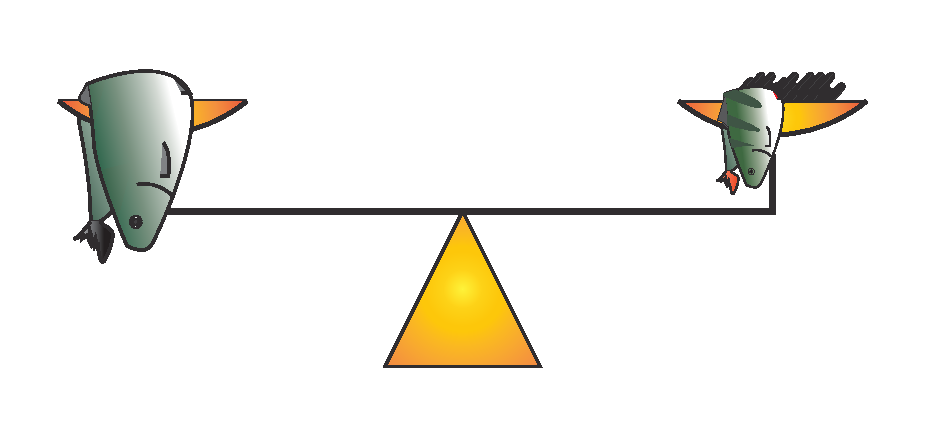
\includegraphics[scale=0.6]{pictures/Kuva10-1-vaaka.pdf} % CC-BY Lilja Tamminen
 %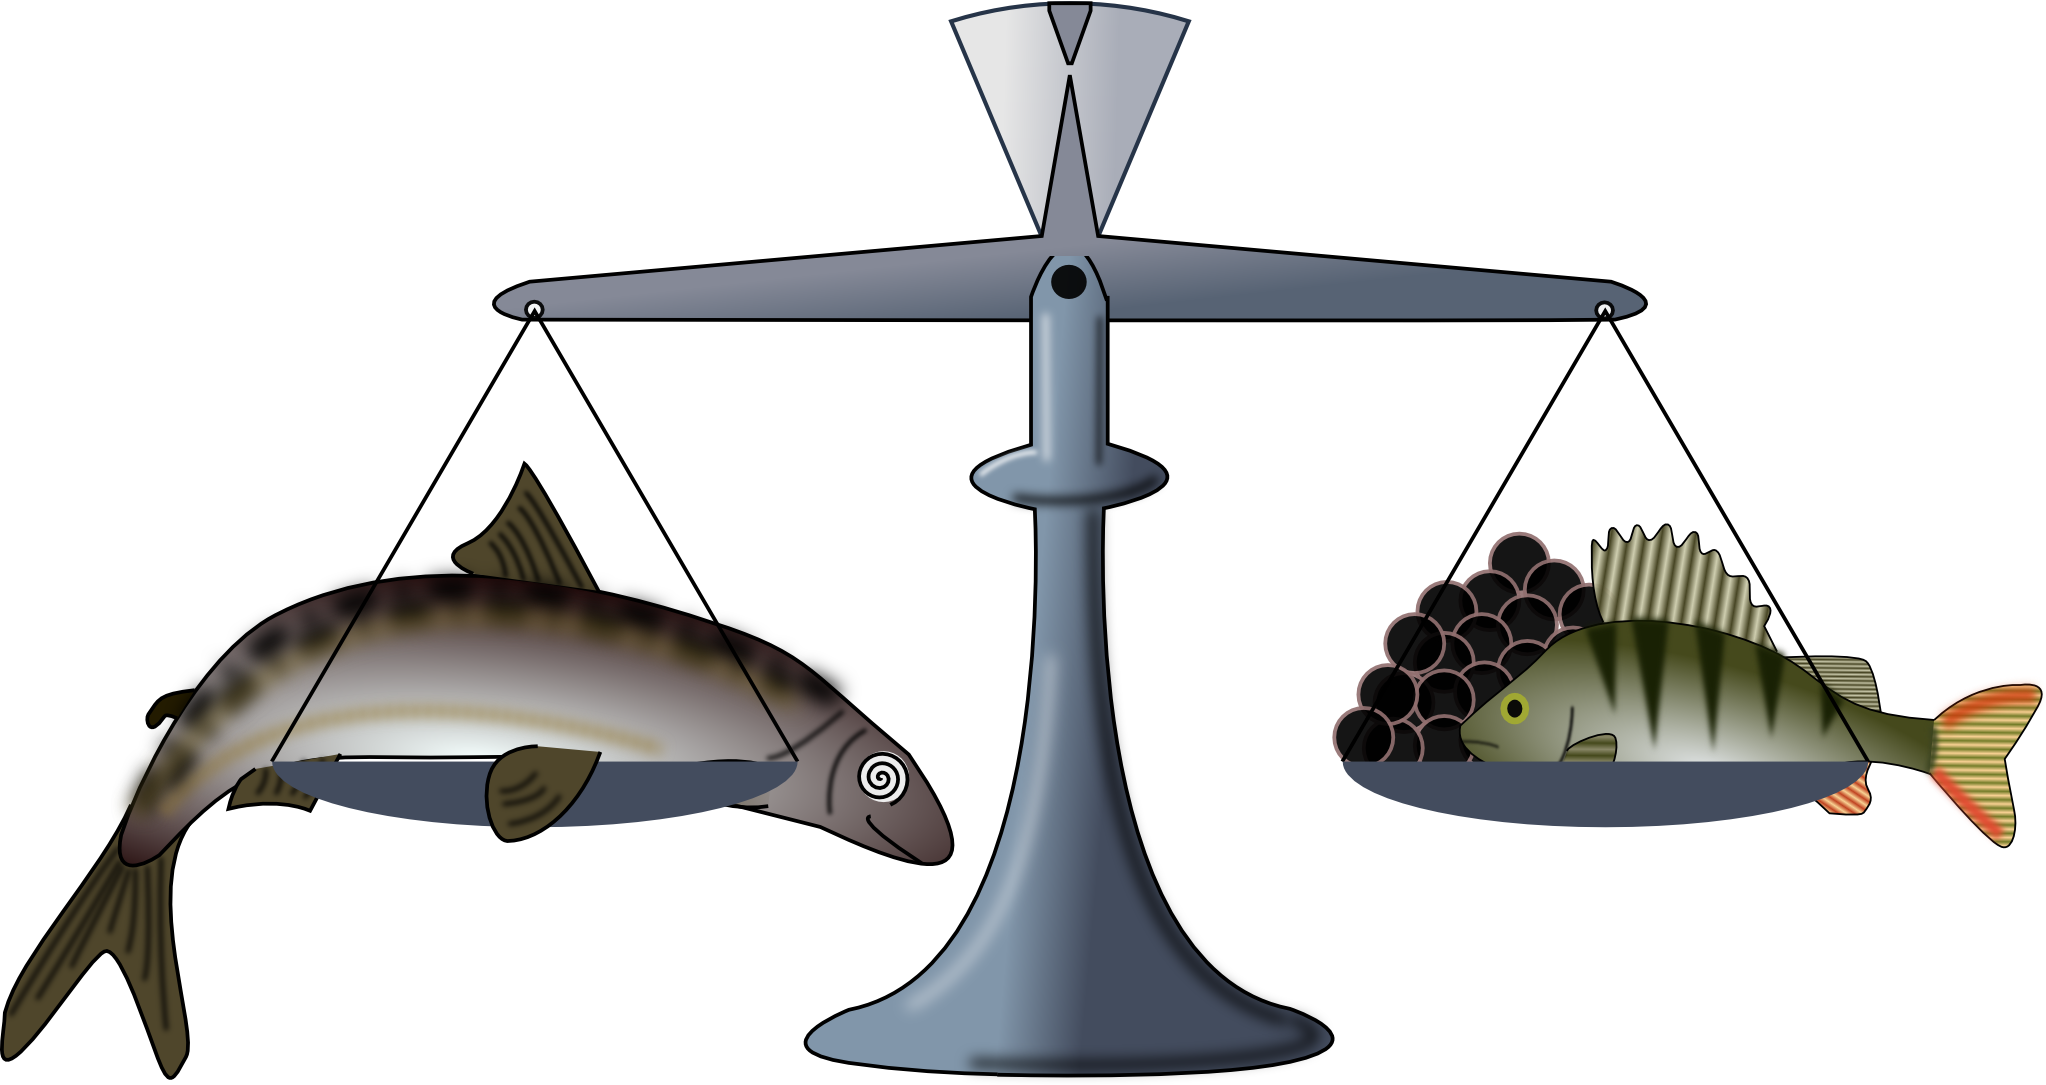
\includegraphics{unused/kala-vaaka.png} % CC-BY Hannu Köngäs
 % FIXME Hannun piirros on viimeistellympi (smoothit värjäykset jne.), Liljan piirros taas konsistentimpi
 % kirjan muun kuvituksen kanssa. Kumpi jätetään? Nyt päällä Liljan kuva.
 \end{center}


\textbf{Ratkaisu.}

Merkitään lakritsin määrää tuntemattomalla $x$. Tilannetta kuvaa yhtälö
\begin{equation*}
2 = 0{,5} + x.
\end{equation*}

Ratkaistaan yhtälö.

\begin{align*}
2 &= 0{,5} + x &&\text{| $-0{,5}$} \\
2 - 0{,5} &= x && \\
1{,5} &= x && \\
x &= 1{,5} && \\
\end{align*}


\textbf{Vastaus.} Lakritsia on $1{,5}$ kg.
\end{esimerkki}

% FIXME \todo{lisää yhtälöesimerkkejä} Laitoin tuon ToDon pois rumentamasta kirjaa.


\laatikko{
\begin{alakohdat}
\alakohta{Yhtälössä esiintyy yleensä \emph{tuntemattomia}, joiden arvoa ei tiedetä ja joita merkitään eri symboleilla. Jos tuntemattomia on vain yksi, sitä merkitään yleensä kirjaimella $x$.}
\alakohta{Niitä tuntemattoman $x$ arvoja, joilla yhtälö pätee, kutsutaan yhtälön \emph{ratkaisuiksi}.}
\alakohta{Yhtälön ratkaisemisella tarkoitetaan kaikkien yhtälön ratkaisujen selvittämistä.}
\end{alakohdat}
}

% FIXME  \todo{jokin helposti ymmärrettävä esimerkki tuntemattomista} Laitoin tuon ToDon pois rumentamasta kirjaa.

\laatikko{
Tyypillinen tapa ratkaista yhtälöitä on kirjoittaa ne ilmaistuna toisella tavalla. Käytännössä tämä tarkoittaa niiden muokkaamista siten, ettei alkuperäisen yhtälön paikkansapitävyys muutu. Tällaisia sallittuja muunnoksia ovat esimerkiksi:
\begin{alakohdat}
\alakohta{Yhtälön molemmille puolille voidaan lisätä tai molemmilta puolilta voidaan vähentää luku. Esimerkiksi yhtälö $3x+5 = 3$ saadaan näin muotoon $3x = -2$.}
\alakohta{Yhtälön molemmat puolet voidaan kertoa nollasta poikkeavalla luvulla. Esimerkiksi kertomalla yhtälön $2x = 4$ molemmat puolet luvulla $\frac{1}{2}$ saadaan yhtälö $x = 2$.}
\end{alakohdat}
}

Kuvitellaan orsivaaka, joka on tasapainossa. Vasemmalla ja oikealla puolella on eripainoisia esineitä, mutta ne painavat yhteensä yhtä paljon. Jos molemmille puolille lisätään nyt saman verran painoa, vaaka on yhä tasapainossa. Samalla tavalla yhtälön molemmille puolille on sallittua lisätä sama luku.

Yhtälöt ratkeavat siten, että niitä muokataan, kunnes vastauksen voi lukea siitä suoraan, esim $x=3$.
%Koska jokaisessa muokkausjonon yhtälössä ratkaisut ovat samat, näin saadaan %alkuperäisen yhtälön ratkaisut.

%%esimerkki tulee 1. asteen yhtälön yhteydessä

\laatikko{
Yhtälöitä on kolmenlaisia:
\begin{alakohdat}
\alakohta{Yhtälö, joka on aina tosi. Esimerkiksi yhtälöt $8=8$ ja $x=x$.}
\alakohta{Yhtälö, joka on joskus tosi. Esimerkiksi yhtälö $x+4=7$ on tosi, kun $x=3$,}
ja epätosi muulloin.
\alakohta{Yhtälö, joka ei ole koskaan tosi. Esimerkiksi yhtälö $0=1$.}
\end{alakohdat}
}

Tärkeimpiä näistä ovat joskus todet yhtälöt.

\laatikko{Yleisiä yhtälönratkaisuperiaatteita:

\begin{alakohdat}
\alakohta{Kerro tuntematonta sisältävät lausekkeet pois nimittäjistä.}
\alakohta{Yhdistä useat murtolausekkeet yhdeksi laventamalla.}
\alakohta{Yhdistä tuntemattomat.}
\alakohta{Kumoa juuret korottamalla yhtälö puolittain sopivaan potenssiin.}
\alakohta{Sulkuja ei välttämättä aina kannata kertoa auki.}
\alakohta{Yhtälö on ratkaistu vasta, kun jäljellä on enää vain yksi kappale tuntematonta suuretta, ja se sijaitsee yksin omalla puolellaan yhtälöä.}


\end{alakohdat}
}

Siirrymme nyt tarkastelemaan tärkeää yhtälöiden lajia, ensimmäisen asteen yhtälöitä.

    \section{Ensimmäisen asteen yhtälö}

\laatikko{
Ensimmäisen asteen yhtälöksi kutsutaan yhtälöä, joka on esitettävissä muodossa $ax+b=0$, jossa $a \neq 0$.
}

Yhtälötyypin nimi tulee siitä, että korkein potenssi, johon tuntematon $x$
yhtälössä korotetaan, on $1$.

\begin{esimerkki}
Muun muassa seuraavat yhtälöt ovat ensimmäisen asteen yhtälöitä:
\begin{alakohdat}
\alakohta{$2x = 4$}
\alakohta{$5x+3 = 0$}
\alakohta{$x+2 = 3x-4$}
\end{alakohdat}
\end{esimerkki}

\laatikko{
Ensimmäisen asteen yhtälö ratkaistaan siirtämällä ensin tuntemattoman $x$ sisältävät termit yhtälön vasemmalle puolelle ja vakiotermit oikealle puolelle. Tämän jälkeen yhtälö jaetaan puolittain tuntemattoman $x$ kertoimella.
}
% FIXME ruma todo-looda taas pois\todo{onko 1. asteen yhtälönratkaisun laatikossa käytettävä ''siirtää toiselle puolelle'' ehkä kuitenkin voi olla noin}

\begin{esimerkki}
Yhtälön $7x+4=4x+7$ ratkaisu saadaan seuraavasti:
\begin{align*}
7x+4 &= 4x+7 & &| \, \text{Vähennetään molemmilta puolilta $4x$.} \\
3x+4 &= 7 & &| \, \text{Vähennetään molemmilta puolilta 4.} \\
3x &= 3 & &| \, \text{Jaetaan molemmat puolet luvulla 3.} \\
x &= 1 & & \\
\end{align*}

\textbf{Vastaus.} $x=1$
\end{esimerkki}

Ensimmäisen asteen yhtälöllä on aina täsmälleen yksi ratkaisu.

Kaikki muotoa $ax+b=cx+d$ olevat yhtälöt, joissa $a \neq c$, ovat ensimmäisen asteen yhtälöitä. Tämä voidaan todistaa seuraavasti:

\begin{align*}
ax+b &= cx+d & &| \, \text{Vähennetään molemmilta puolilta $cx+d$}. \\
ax+b - (cx+d) &= 0 & &| \, \text{Järjestellään termejä uudelleen.} \\
ax - cx + b - d &= 0 & &| \, \text{Otetaan yhteinen tekijä.} \\
(a-c)x + (b-d) &= 0 & &
\end{align*}

Tämä on määritelmän mukainen ensimmäisen asteen yhtälö, koska $a \neq c$.

\begin{esimerkki}
Yleinen lähestymistapa muotoa $ax+b = cx+d$ olevien yhtälöiden ratkaisuun: \\
(1) Vähennä molemmilta puolilta $cx$. Saat yhtälön $(a-c)x + b = d$. \\
(2) Vähennä molemmilta puolilta $b$. Saat yhtälön $(a-c)x = d-b$. \\
(3) Jaa molemmat puolet lausekkeella $(a-c)$. Saat yhtälön ratkaistuun muotoon $x = \frac{d-b}{a-c}$.
\end{esimerkki}

\begin{tehtavasivu}

\begin{tehtava}
Onko $-2$ yhtälön $3x-4 = 7-2x$ ratkaisu?
\begin{vastaus}
Ei ole.
\end{vastaus}
\end{tehtava}

\begin{tehtava}
Mitä yhtälölle $ax+b = 0$ tapahtuu, jos kerroin $a$ saa arvon nolla?
Onko yhtälöllä ratkaisuja?
\begin{vastaus}
Jos $b = 0$, yhtälö toteutuu kaikilla $x$:n arvoilla. Jos $b \neq 0$, yhtälö
ei toteudu millään $x$:n arvolla. Periaatteessa kyseessä ei kuitenkaan
enää ole ensimmäisen asteen yhtälö, mikäli $a = 0$
\end{vastaus}
\end{tehtava}

\begin{tehtava}
%
Ratkaise:
\begin{alakohdat}
\alakohta{$x + 4 = 5$}
\alakohta{$1 - x = -3$}
\alakohta{$7x = 35$}
\alakohta{$-2x = 4$}
\alakohta{$10 - 2x = x$}
\alakohta{$9x + 4 = 6 - x$}
\alakohta{$\frac{2x}{5} = 4$}
\alakohta{$\frac{x}{3} + 1 = \frac{5}{6} - x$}
\end{alakohdat}
\begin{vastaus}
\begin{alakohdat}
\alakohta{$x=1$}
\alakohta{$x=4$}
\alakohta{$x=35/7$}
\alakohta{$x=-2$}
\alakohta{$x=10/3$}
\alakohta{$x=1/5$}
\alakohta{$x=10$}
\alakohta{$x=-1/8$}
\end{alakohdat}
\end{vastaus}
\end{tehtava}

\begin{tehtava}
Ratkaise yhtälö. Tarkista laskimella tai tietokoneella.
\begin{alakohdat}
    \alakohta{$-2x+5=2(5+x)$}
    \alakohta{$4(x-1) - 3x = 15-4x$}
    \alakohta{$6 - (2x+3) = 3-2x$}
    \alakohta{$x - 100\,000 = -0,25x$}
    \alakohta{$10^6 x - 3 \cdot 10^9 = 0$}
    \alakohta{$5(1-x) = -5x+3$}
\end{alakohdat}
%
\begin{vastaus}
\begin{alakohdat}
    \alakohta{$x=-\frac 5 4$}
    \alakohta{$x=\frac{19}{5}$}
    \alakohta{Yhtälö toteutuu kaikilla reaaliluvuilla.}
    \alakohta{$x=80\,000$}
    \alakohta{$x=3000$}
    \alakohta{Yhtälö ei toteudu millään reaaliluvulla.}
\end{alakohdat}
%
\end{vastaus}
\end{tehtava}





\begin{tehtava}
Ratkaise kysytty tuntematon yhtälöstä
\begin{alakohdat}
\alakohta{$F=ma$, $m=?$ (Voima on massa kerrottuna kiihtyvyydellä.)}
\alakohta{$p=\frac{F}{A}$, $F=?$ (Paine on voima jaettuna alalla.)}
\alakohta{$A=\pi r^2$, $r=?$ (Ympyrän pinta-ala on pii kerrottuna säteen neliöllä.)}
\alakohta{$V=\frac{1}{3} \pi r^2 h$, $h=?$ (Kartion tilavuus on piin kolmasosa}
kerrottuna säteen neliöllä ja kartion korkeudella.)
\end{alakohdat}
\begin{vastaus}
\begin{alakohdat}
\alakohta{$m=\frac{F}{a}$}
\alakohta{$F=p A$}
\alakohta{$r=\sqrt{\frac{A}{\pi}}$}
\alakohta{$h=\frac{V}{ \frac{1}{3} \pi r^2 h}$}
\end{alakohdat}
\end{vastaus}
\end{tehtava}

\begin{tehtava}
Ratkaise yhtälö. Tarkista laskimella tai tietokoneella.
\begin{alakohdat}
    \alakohta{$\dfrac{8x}{3} = 12$}
    \alakohta{$3 - \dfrac{x}{4} = x$}
    \alakohta{$-\dfrac{7x}{8} = x+2$}
    \alakohta{$x+7 = 1 - \dfrac{x-1}{2}$}
    \alakohta{$\dfrac{2x-1}{3} - 1 = \dfrac{4x}{9}$}
    \alakohta{$\dfrac{x+5}{3} = x+3-\dfrac{2x+1}{4}$}
\end{alakohdat}
%
\begin{vastaus}
\begin{alakohdat}
    \alakohta{$x=4\frac 1 2$}
    \alakohta{$x=2\frac{2}{5}$}
    \alakohta{$x=-1\frac{1}{15}$}
    \alakohta{$x = -3\frac 2 3$}
    \alakohta{$x=6$}
    \alakohta{$x=-6\frac{1}{2}$}
\end{alakohdat}
\end{vastaus}
\end{tehtava}


\begin{tehtava}
Huvipuistossa yksittäinen laitelippu maksaa 7 euroa, ja sillä pääsee yhteen laitteeseen. Rannekkeella pääsee käymään päivän aikana niin monessa laitteessa kuin haluaa, ja se maksaa 37 euroa. Kuinka monessa laitteessa on käytävä, jotta rannekkeen ostaminen kannattaa?
\begin{vastaus}
$6$ laitteessa
\end{vastaus}
\end{tehtava}

\begin{tehtava}
Kännykkäliittymän kuukausittainen perusmaksu on 2,90 euroa. Lisäksi jokainen puheminuutti ja tekstiviesti maksaa 0,69 senttiä. Pekan kännykkälasku kuukauden
ajalta oli 27,05 euroa.

\begin{alakohdat}
	\alakohta{Kuinka monta puheminuuttia/tekstiviestiä Pekka käytti kuukauden aikana?}
	\alakohta{Pekka lähetti kaksi tekstiviestiä jokaista viittä puheminuuttia kohden. Kuinka monta tekstiviestiä Pekka lähetti?}
\end{alakohdat}

	\begin{vastaus}
		\begin{alakohdat}
			\alakohta{350 puheminuuttia/tekstiviestiä}
			\alakohta{100 tekstiviestiä}
		\end{alakohdat}
	\end{vastaus}
\end{tehtava}

\begin{tehtava}
Sadevesikeräin näyttää vesipatsaan korkeuden millimetreinä. Eräänä aamuna
keräimessä oli 5~mm vettä. Seuraavana aamuna samaan aikaan keräimessä oli 23~mm vettä. Muodosta yhtälö ja selvitä, kuinka paljon vettä oli keskimäärin satanut kuluneen vuorokauden aikana tunnissa.
	\begin{vastaus}
	$0,75$ mm/tunti
	\end{vastaus}
\end{tehtava}

\begin{tehtava}
Määritä luvulle $a$ sellainen arvo, että yhtälön $5x-8-3ax=4-x$ ratkaisu on $-1$.
\begin{vastaus}
$a=6$
\end{vastaus}
\end{tehtava}

\begin{tehtava}
Kylpyhuoneessa on kolme hanaa. Hana A täyttää kylpyammeen 60 minuutissa, hana B 30 minuutissa ja hana C 15 minuutissa. Kuinka kauan kylpyammeen täyttymisessä kestää, jos kaikki hanat ovat yhtäaikaa auki?
\begin{vastaus}
$8$ min $34$ s
\end{vastaus}
\end{tehtava}

\end{tehtavasivu}

    \section{Suoraan ja kääntäen verrannollisuus}

Kaksi muuttujaa voivat riippua toisistaan monin eri tavoin. Tavallisia
riippuvuuden tyyppejä ovat suoraan ja kääntäen verrannollisuus.

\laatikko{
Kaksi muuttujaa $x$ ja $y$ ovat suoraan verrannolliset, jos toinen saadaan
toisesta kertomalla se jollakin vakiolla, eli $y = kx$. Vakiota $k$
kutsutaan \emph{verrannollisuuskertoimeksi}.}

Jos suureet $x$ ja $y$ ovat suoraan verrannolliset, niin tätä merkitään $x\sim y$ tai $x\propto y$.

Suoraan verrannollisuus voidaan tunnistaa esimerkiksi laskemalla muuttujien
suhde ja toteamalla, että se on muuttujista riippumaton vakio.

\begin{esimerkki}
Banaanien kilohinta on $2,00$ euroa. Seuraavassa taulukossa on
banaanien paino\footnote{Fysikaalisesti kyse on massasta, mutta
arkikielessä käytetään sanaa paino.}, jonka saa ostettua tietyllä rahamäärällä:
\begin{center} 
\begin{tabular}{|l|r|r|}
\hline
Hinta (euroa) & Paino (kg) & Hinta/paino (euroa/kg) \\
\hline
$1,00$ & $0,50$ & $2,00$ \\
$2,00$ & $1,00$ & $2,00$ \\
$3,00$ & $1,50$ & $2,00$ \\
$4,00$ & $2,00$ & $2,00$ \\
\hline
\end{tabular}
\end{center}
Hinnan ja painon suhde on vakio, $2,00$ euroa/kg, joten ostettujen
banaanien paino ja niihin käytetty rahamäärä ovat suoraan verrannolliset.
\end{esimerkki}

Suoraan verrannollisuutta voidaan kuvata myös niin, että jos
toinen muuttujista kaksinkertaistuu, niin toinenkin kaksinkertaistuu.
Samoin jos toisen muuttujan arvo puolittuu, toisenkin arvo puolittuu.

Jos suoraan verrannollisista muuttujista piirretään kuvaaja, pisteet
asettuvat suoralle:

%\missingfigure{Kuva, johon piirretty vaaka-akselille käytetty rahamäärä
%ja pystyakselille ostettujen banaanien paino.}

\begin{center}
\begin{kuvaajapohja}{1.5}{0}{5}{0}{3}
\kuvaajapiste{1}{0.5}
\kuvaajapiste{2}{1}
\kuvaajapiste{3}{1.5}
\kuvaajapiste{4}{2}
\kuvaaja{0.5*x}{}{black}
\node at (8.2,0) {euroa};
\node at (0,4.8) {kg};
\end{kuvaajapohja}
\end{center}

Suoraan verrannollisia muuttujia ovat myös esimerkiksi
\begin{alakohdat}
    \alakohta{aika ja kuljettu matka, kun liikutaan vakionopeudella, tai}
    \alakohta{kappaleen massa ja painovoiman kappaleeseen aiheuttama voima.}
\end{alakohdat}

Suoraan verrannollisuutta monimutkaisempi riippuvuus on kääntäen
verrannollisuus.

\laatikko{
Muuttujat $x$ ja $y$ ovat kääntäen verrannolliset, jos toinen saadaan toisesta
jakamalla jokin vakio sillä, eli $y = \frac{a}{x}$.
}

Kääntäen verrannollisuus voidaan tunnistaa esimerkiksi
kertomalla muuttujien arvoja keskenään ja huomaamalla,
että tulo on muuttujista riippumaton vakio.

\begin{esimerkki}
Nopeus ja matkaan tarvittava aika ovat kääntäen verrannolliset.
Jos kuljettavana matkana on $10$ km, voidaan nopeudet ja matka-ajat
kirjoittaa taulukoksi:
\begin{center} 
\begin{tabular}{|l|r|r|}
\hline
Nopeus (km/h) & Matka-aika (h) & Nopeus$\cdot$matka-aika (km) \\
\hline
$5$ & $2$ & $10$ \\
$10$ & $1$ & $10$ \\
$12$ & $0,8$ & $10$ \\
\hline
\end{tabular}
\end{center}
Tulo on aina $10$ km, joten nopeus ja matka-aika ovat kääntäen verrannolliset.
\end{esimerkki}

Kääntäen verrannollisuutta voidaan kuvata myös niin, että jos
toinen muuttujista kaksinkertaistuu, toinen puolittuu.

Jos kääntäen verrannollisista muuttujista piirretään kuvaaja, pisteet
muodostavat laskevan käyrän:

%\missingfigure{Kuva, johon on piirretty matka-aika ja nopeus (yllä olevan
%taulukon mukaisesti).}

% FIXME sellainen käyrätemplate, joka toimii myös silloin, jos toiseen akseliin
% FIXME tarvitaan eri jakoväli kuin toiseen.
% FIXME Myös akseleiden nimeäminen olisi kiva olla templatessa.
\begin{center}
\begin{kuvaajapohja}{0.8}{0}{13}{0}{5}
\kuvaajapiste{5}{2}
\kuvaajapiste{10}{1}
\kuvaajapiste{12}{0.8}
\kuvaaja{10/x}{}{black}
\node at (10.6,0) {h};
\node at (0,4.3) {km/h};
\end{kuvaajapohja}
\end{center}


Kääntäen verrannollisia muuttujia ovat myös esimerkiksi
\begin{alakohdat}
    \alakohta{kaivamistyön suorittamiseen kuluva aika ja työntekijöiden lukumäärä.}
\end{alakohdat}

\begin{tehtavasivu}

\begin{tehtava}
    Tutkitaan seuraavia muuttujapareja:
    \begin{alakohdat}
        \alakohta{Neliön sivun pituus ja neliön pinta-ala.}
        \alakohta{Kuljettu matka ja kulunut aika, kun nopeus on vakio.}
        \alakohta{Dieselin hinta ja 50 eurolla saatavan dieselin määrä.}
        \alakohta{Irtomyynnistä ostetun suolakurkkuerän paino ja hinta.}
    \end{alakohdat}
    Miten toinen muuttuja muuttuu ensimmäisen kaksinkertaistuessa tai puolittuessa? Ovatko muuttujat suoraan tai kääntäen verrannolliset vai eivät kumpaakaan?
    \begin{vastaus}
        Vastaus:
        \begin{alakohdat}
            \alakohta{Eivät ole.}
            \alakohta{Suoraan verrannolliset.}
            \alakohta{Kääntäen verrannolliset.}
            \alakohta{Suoraan verrannolliset.}
        \end{alakohdat}
    \end{vastaus}
\end{tehtava}

\begin{tehtava}
Ratkaise
\begin{alakohdat}
\alakohta{$ \frac{x}{3} = 1$}
\alakohta{$ \frac{8}{x} = 2$}
\alakohta{$ \frac{7}{x} = \frac{16}{8}$}
\alakohta{$ \frac{x}{3} = \frac{1}{7}$}
\end{alakohdat}
\begin{vastaus}
\begin{alakohdat}
\alakohta{$x= \frac{1}{3}$}
\alakohta{$y= \frac{1}{4}$}
\alakohta{$x= \frac{7}{2}$}
\alakohta{$x= \frac{3}{7}$}
\end{alakohdat}
\end{vastaus}
\end{tehtava}

\begin{tehtava}
Muodosta seuraavia tilanteita kuvaavat yhtälöt. 
%Voit käyttää vakion merkkinä esimerkiksi kirjainta $c$. %%%miksei vakiintunutta k:ta?
\begin{alakohdat}
\alakohta{Kultakimpaleen arvo ($x$) on suoraan verrannollinen sen massaan ($m$), eli mitä painavampi kimpale on, sitä enemmän siitä saa rahaa.}
\alakohta{Aidan maalaamiseen osallistuvien ihmisten määrä {$x$} on kääntäen verrannollinen maalaamiseen kuluvaan aikaan ($t$). Toisin sanoen, mitä}
enemmän maalaajia, sitä nopeammin homma on valmis.
\alakohta{Planeettojen toisiinsa aiheuttama vetovoima ($F$) on suoraan verrannollinen planeettojen massoihin ($m_1$ ja $m_2$) ja kääntäen verrannollinen niiden välisen etäisyyden ($r$) neliöön.}
\end{alakohdat}
\begin{vastaus}
\begin{alakohdat}
\alakohta{$ \frac{x}{m}=c$}
\alakohta{$ xt=c $}
\alakohta{$ \frac{Fr^2}{m_1+m_2}=c$}
\end{alakohdat}
\end{vastaus}
\end{tehtava}

\begin{tehtava}
Rento pyöräilyvauhti kaupunkiolosuhteissa on noin $20$~km/h. Lukiolta urheiluhallille on matkaa $7$~km. Kuinka monta minuuttia kestää arviolta pyöräillä lukiolta urheiluhallille?
\begin{vastaus}
Viiden minuutin tarkkuudella $20$ min.
\end{vastaus}
\end{tehtava}

\begin{tehtava}
    Isä ja lapset ovat ajamassa mökille Sotkamoon. On ajettu jo neljä
    viidesosaa matkasta, ja aikaa on kulunut kaksi tuntia. ''Joko ollaan perillä?''
    lapset kysyvät takapenkiltä. Kuinka pitkään vielä arviolta kuluu, ennen
    kuin ollaan mökillä?
    
    \begin{vastaus}
        Vastaus: 30 min
    \end{vastaus}
\end{tehtava}

\begin{tehtava}
    Äidinkielen kurssilla annettiin tehtäväksi lukea 300-sivuinen romaani.
    Eräs opiskelija otti aikaa ja selvitti lukevansa vartissa seitsemän sivua.
    Kuinka monta tuntia häneltä kuluu koko romaanin lukemiseen, jos
    taukoja ei lasketa?
    
    \begin{vastaus}
        Vastaus: 642 minuuttia eli 10 h 42 min.
    \end{vastaus}
\end{tehtava}

\begin{tehtava}
Alkuperäiskansojen perinteitä tutkiva etnologi kerää saamelaisten kansantarinoita. Kierrettyään viikkojen ajan saamelaisperheiden vieraana palaa etnologi yliopistolle mukanaan äänitiedostoiksi tallennettuja haastatteluja. Jotta etnologi voi ryhtyä kirjoittamaan tutkimusraporttia, pitää haastattelutiedostot ensin purkaa tekstiksi eli \emph{litteroida.} Tähän etnologi pyytää apua laitoksen opiskelijoilta. Neljä opiskelijaa litteroi tiedostot 25~tunnissa. Kuinka kauan aikaa kuluu, jos työhön saadaan vielä kolme opiskelijaa lisää? Kuinka monta opiskelijaa tarvitaan, jotta työ saataisiin tehdyksi 9~tunnissa? Oletetaan, että kaikkien opiskelijoiden työteho on sama.

\begin{vastaus}
Seitsemällä opiskelijalla työ valmistuu noin 14~tunnissa. Työ valmistuu 8~tunnissa, jos opiskelijoita on  12.
\end{vastaus}
\end{tehtava}

\begin{tehtava}
Kappaleen liike-energia on suoraan verrannollinen nopeuden neliöön. Kun kappale liikkui nopeudella 9,0~m/s, sillä oli 150~joulea liike-energiaa. Laske kappaleen liike-energia, kun sen nopeus on 5,0~m/s. 
\begin{vastaus}
46~J
\end{vastaus}
\end{tehtava}


\begin{tehtava}
	10 miestä kaivaa 10 kuoppaa 10 tunnissa. 
%	Kuinka kauan viidellä miehellä kestää kaivaa puolikas kuoppa?
	Kuinka kauan viidellä miehellä kestää kaivaa 20 kuoppaa?
	
	\begin{vastaus}
		Vastaus: 40 tuntia
	\end{vastaus}	
\end{tehtava}

\end{tehtavasivu}

    \section{Prosenttilaskenta}

Sana prosentti tulee latinan kielen sanoista \emph{pro centum}, mikä tarkoittaa kirjaimellisesti sataa kohden. Prosentteja käytetään ilmaisemaan suhteellista osuutta. Prosentin merkki on \%.


\laatikko{1~prosentti $= 1~\% = \frac{1}{100} = 0,01$}

\begin{esimerkki}
\mbox{}
\begin{itemize}
  \item $6~\% = \frac{6}{100} = 0,06$
  \item $48,2~\% = \frac{48,2}{100} = 0,482$
  \item $140~\% = \frac{140}{100} = 1,40$ 
\end{itemize}
\end{esimerkki}

% FIXME \todo{tehtävä: ilmaise desimaalilukuna seuraavat prosentit}

%%%%PERUSARVO%%%%%%%
\laatikko{
Lukua, josta suhde lasketaan, kutsutaan \emph{perusarvoksi}.
}


\begin{esimerkki}
Jos sadan euron hintaisen tuotteen hintaa on alennettu 25 prosenttia, niin alennettu hinta on 75 euroa. Jos sen sijaan alkuperäinen hinta nousee 15 prosenttia, niin tuotteen uusi hinta on 115 euroa. Perusarvo on molemmissa tapauksissa 100 euroa.

%\missingfigure{kuva suorakaiteesta, joka kuvaa perusarvoa (se voi olla vaik 10x10 pientä laatikkoa. Sit kuva, jossa peruarvosta on vähennetty 25~\% perusarvosta, eli 75 laatikkoa. Sit kuva, jossa perusarvoon on lisätty 15~\%, eli 115 laatikkoa. Sit sopivat havainnollistavat väritykset}

\begin{center}
 
\includegraphics[scale=.25]{pictures/Kuva13-1-100.pdf}
 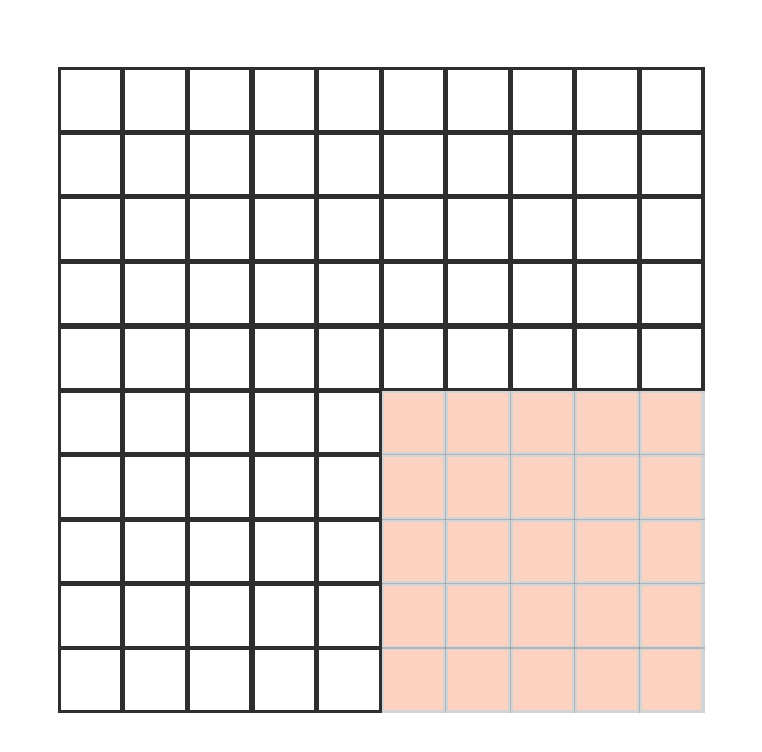
\includegraphics[scale=.25]{pictures/Kuva13-2-75.pdf}
 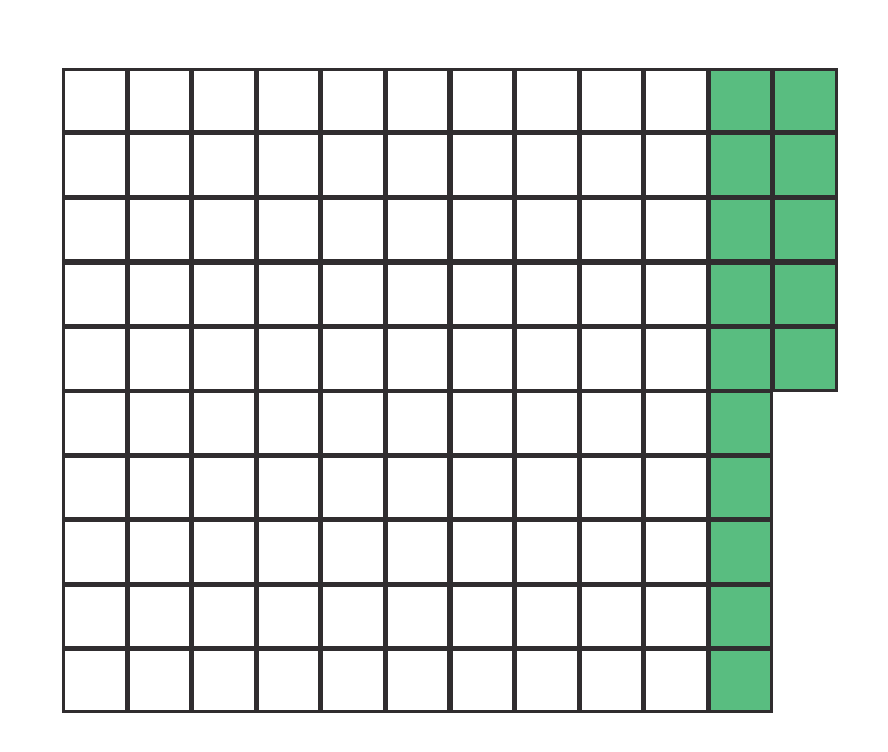
\includegraphics[scale=.25]{pictures/Kuva13-3-115.pdf}
\end{center}


\end{esimerkki}


% FIXME \todo{tehtävä perusarvosta}


%MUUTOSPROSENTTITEORIA
\laatikko{
Prosentteja käytetään usein ilmaisemaan suureiden muutoksia, esimerkiksi luku $b$ kasvaa luvuksi $a$. \emph{Muutosprosenttia} laskettaessa muutoksen suuruutta verrataan alkuperäiseen lukuun. Perusarvona on siis alkuperäinen arvo, johon nähden muutos on tapahtunut.

Jos kysytään, kuinka monta prosenttia $a$ on isompi $b$:tä, se tarkoittaa samaa, kuin kuinka monta $b$:n sadasosaa on se määrä, jolla $a$ on suurempi $b$:tä. Toisin sanoen kuinka monta $b$:n sadasosaa mahtuu $a-b$:hen. Se saadaan laskemalla

\begin{equation*}
\frac{a-b}{\frac{b}{100}} = \frac{a-b}{b} \cdot 100
\end{equation*}

Samalla tavalla saadaan laskettua, kuinka monta prosenttia luku kasvoi, kun se muuttui $a$:sta $b$:hen.
}




%TÄMÄ ON MUUTOSPROSENTTITEHTÄVÄESIMERKKI
\begin{esimerkki}
Vesan paino on tammikuussa 68~kg ja kesäkuussa 64~kg. Kuinka monta prosenttia Vesa on laihtunut?

\textbf{Ratkaisu.}

Lasketaan 
\begin{equation*}
\frac{68-64}{68}\cdot 100~\% = \frac{4}{68} \cdot 100~\%=0,06\cdot 100~\% = 6~\% 
\end{equation*}

\textbf{Vastaus.}

Vesa on laihtunut $6~\%$.
\end{esimerkki}

\begin{tehtava}

Oppikirjamaraton-tiimi kävi lounastamassa. Osoita oheisen kuitin tiedoilla vääräksi yleinen virhekäsitys, että 13 \%:n arvonlisävero olisi 13~\% lopullisesta myyntihinnasta.
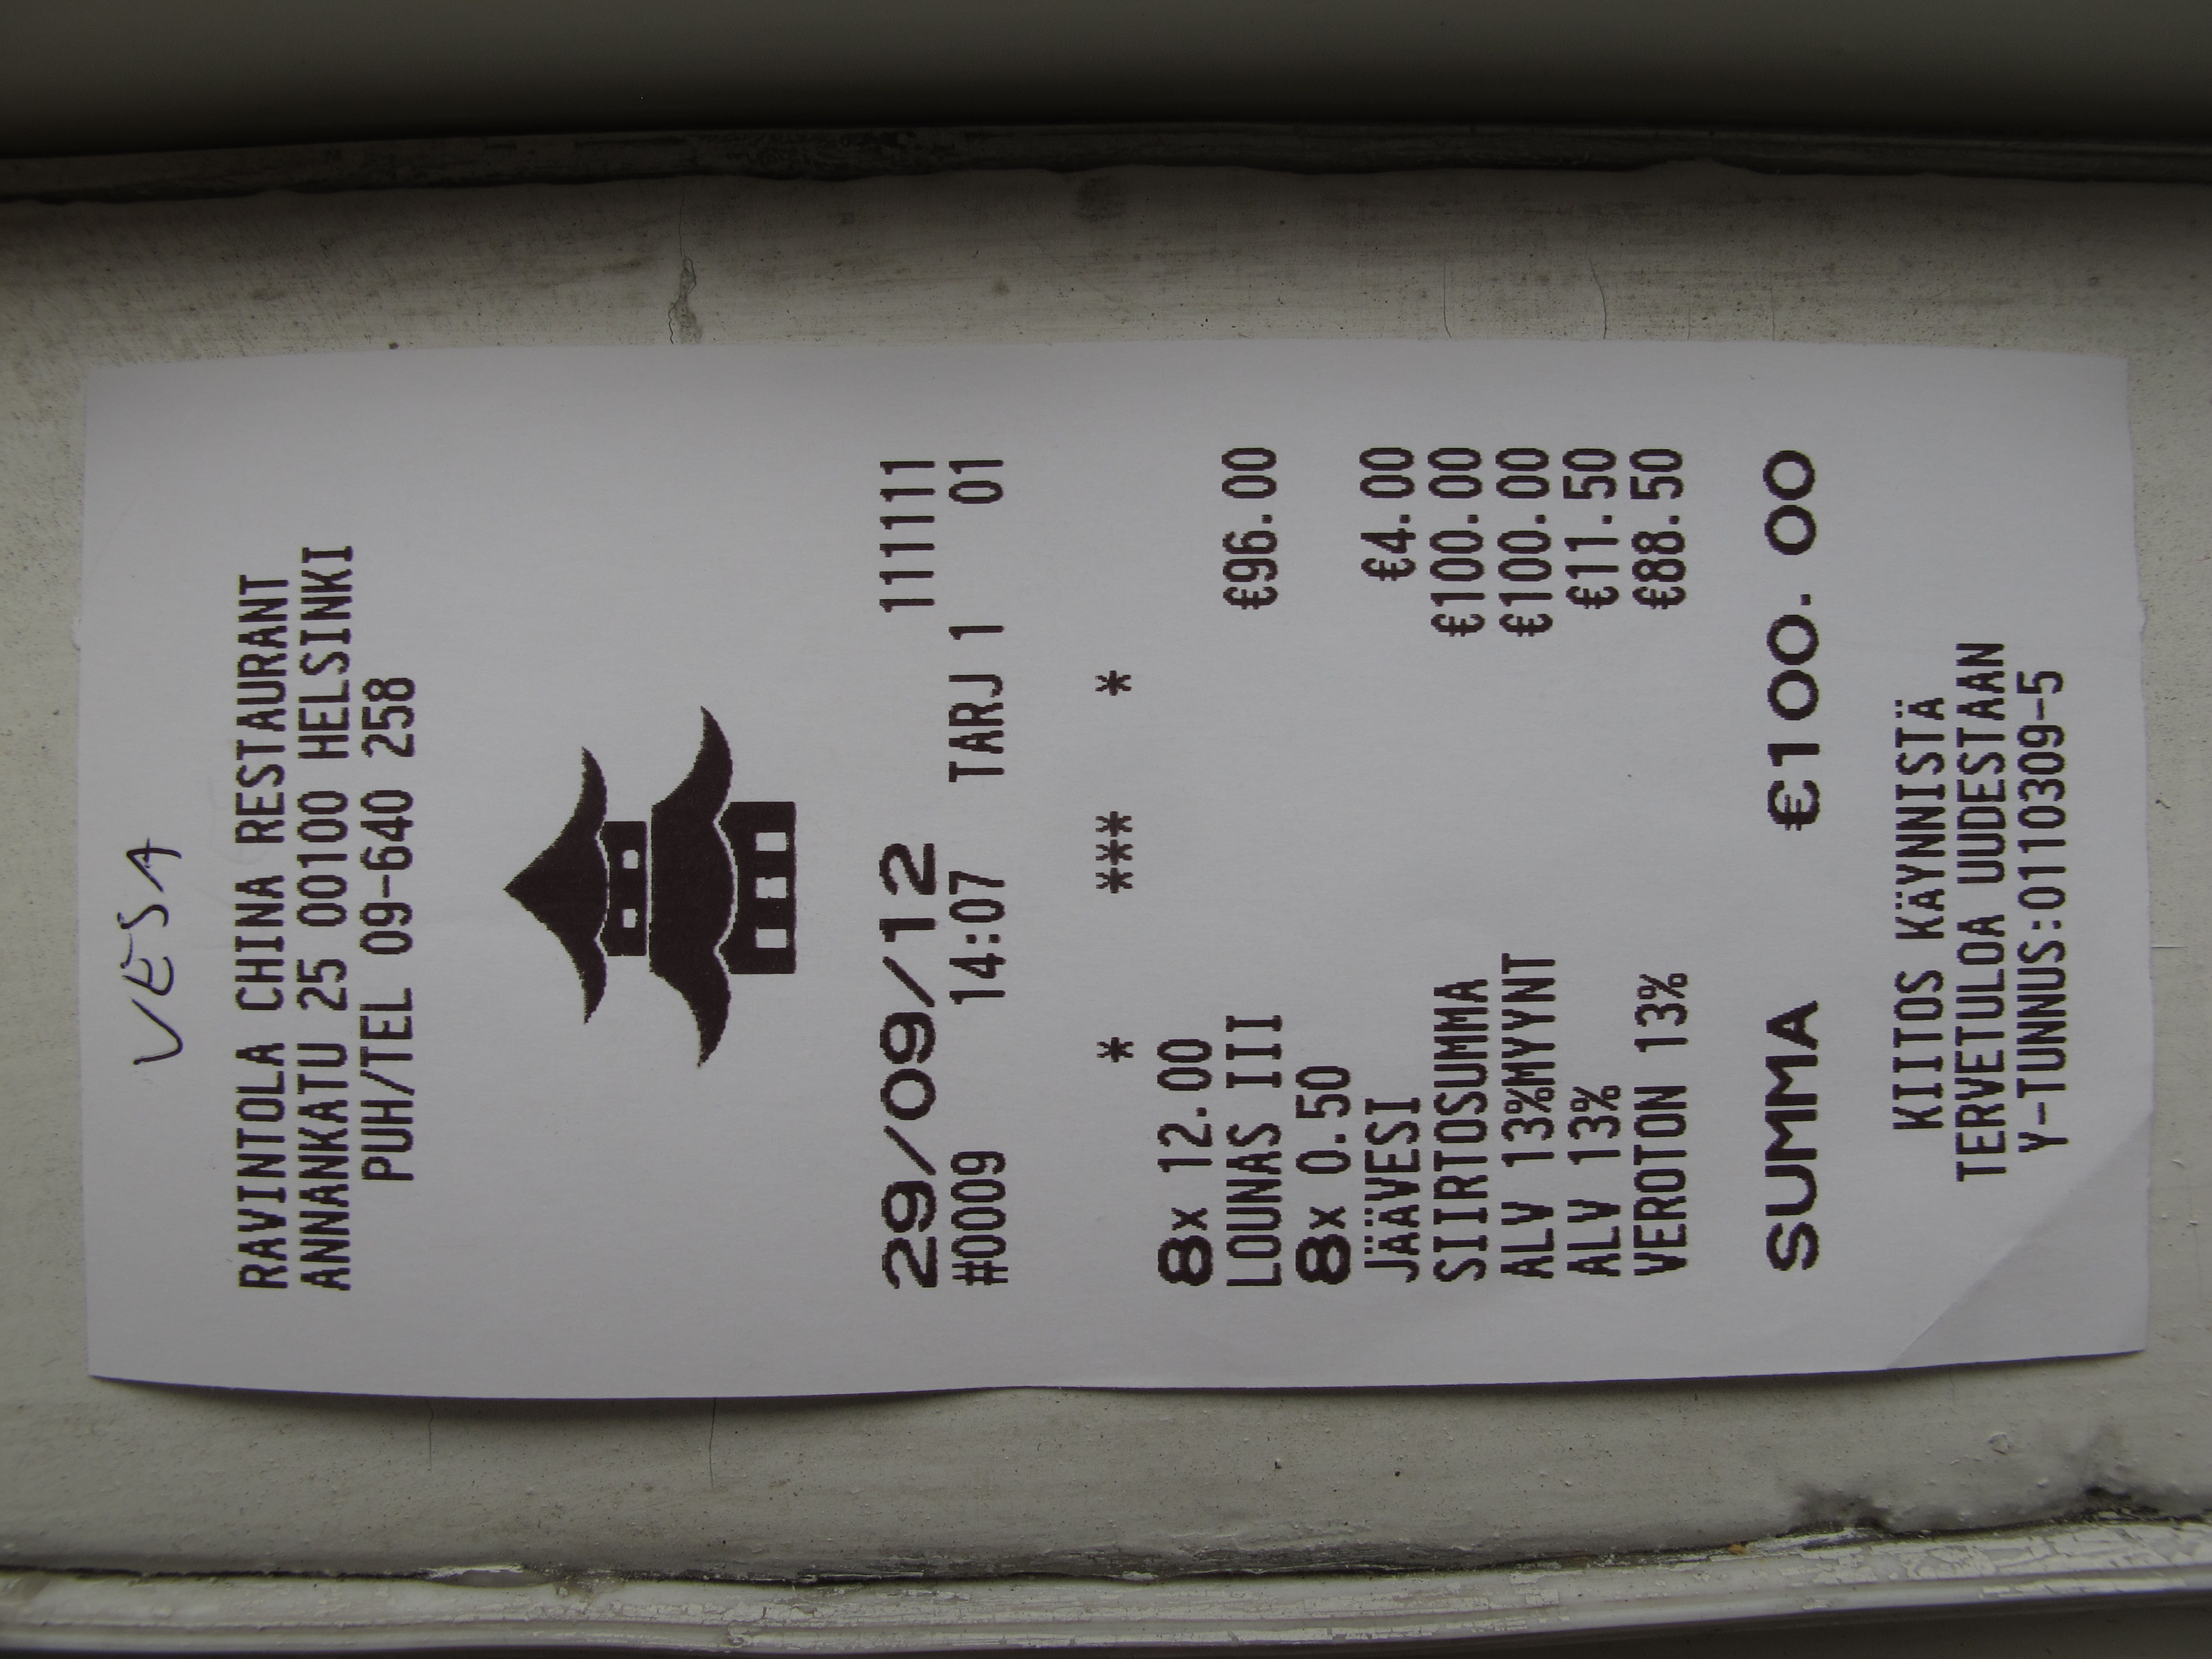
\includegraphics[width=80mm, angle=270]{pictures/alv-kuitti}

\begin{vastaus}
13~\% sadasta eurosta on 13 euroa, ei 11,50 euroa, niin kuin kuitissa todetaan.
\end{vastaus}


\end{tehtava}


%%%VERTAILUPROSENTTI%%%%%
\laatikko{
\emph{Vertailuprosentilla} ilmaistaan, kuinka monta prosenttia luku on jostain toisesta luvusta. Vertailuprosentin laskennassa käytetään perusarvona sitä lukua, johon verrataan.

Jos kysytään, kuinka monta prosenttia $b$ on $a$:stä, se tarkoittaa samaa, kuin kuinka monta $a$:n sadasosaa $b$ on. Toisin sanoen kuinka monta $a$:n sadasosaa $b$:hen mahtuu. Se saadaan laskemalla 

\begin{equation*}
\frac{b}{\frac{a}{100}} = \frac{b}{a} \cdot 100
\end{equation*}

% FIXME: millainen? \missingfigure{havainnollistava kuva vertailuprosentista suorakulmioiden avulla}
}

%TÄMÄ ON VERTAILUPROSENTTITEHTÄVÄESIMERKKI
\begin{esimerkki}
Vesa ansaitsee kuukaudessa ${2~300}$ euroa ja Antero ${1~700}$ euroa. Kuinka monta prosenttia Anteron tulot ovat Vesan tuloista? 

\textbf{Ratkaisu.}

Lasketaan

\begin{equation*}
\frac{1700}{2300} \cdot 100~\%  \approx 0,74\cdot 100~\% = 74~\%. 
\end{equation*}

Laskuissa käytettävä perusarvo on Vesan palkka eli 2~300 euroa.
    
\textbf{Vastaus.}

$74~\%$
\end{esimerkki}



%%%%PROSENTTIYKSIKKÖ
\laatikko{
\emph{Prosenttiyksikkö} mittaa prosenttiosuuksien välisiä eroja. Esimerkiksi $4~\%$ on $2$ prosenttiyksikköä suurempi kuin $2~\%$, mutta $100~\%$ suurempi kuin $2~\%$. Jos prosenttiluku muuttuu, muutos voidaan ilmaista joko prosentteina tai prosenttiyksikköinä.
}


%%%%%%PROSENTTIYKSIKKÖTEHTÄVÄESIMERKKI
\begin{esimerkki}
    Tuotteen markkinaosuus on vuoden tammikuussa 10~\% ja kesäkuussa 15~\%. 
    \begin{enumerate}[a)]
    \item Kuinka monta prosenttia tuotteen markkinaosuus on noussut?
    
    \item Kuinka monta prosenttiyksikköä tuotteen markkinaosuus on noussut?
    \end{enumerate}
    
    {\bf Ratkaisu.} 
    
    \begin{enumerate}[a)]
    \item Tuotteen markkinaosuus on noussut
    \[
    \frac{15-10}{10} \cdot 100~\%= \frac{5}{10}\cdot 100~\% = 50~\%.
    \]
    
    \item Tuotteen markkinaosuus on noussut $15-10=5$ prosenttiyksikköä. 
    \end{enumerate}
    
    {\bf Vastaus.}
    
    \begin{enumerate}[a)]
    \item 50 prosenttia
    \item 5 prosenttiyksikköä.
    \end{enumerate}
\end{esimerkki}

\subsection*{Tehtäviä}

\begin{tehtava}
    Laukun normaalihinta on 225 euroa, ja se on 25~\%:n alennuksessa.
    Mikä on alennettu hinta?
    \begin{vastaus}
    Vastaus: 168,75 euroa
    \end{vastaus}
\end{tehtava}

\begin{tehtava}
    Jaakon kuukausipalkka on 1623,52 euroa. Hän saa 1,3~\% palkankorotuksen.
    Mikä on Jaakon kuukausipalkka korotuksen jälkeen?
    \begin{vastaus}
    1644,63 euroa
    \end{vastaus}
\end{tehtava}
% FIXME alla käytetään euromerkkiä \euro, muualla sanallista muotoa
% ''euro''. Konsistenssin vuoksi voisi valita jomman kumman. 
% Yllä oleva sliedeksen. En pidä pahana ongelmana, että on molempia.
\begin{tehtava}
    Kirjan myyntihinta, joka sisältää arvolisäveron, on 9~\% suurempi kuin kirjan veroton hinta. Laske kirjan veroton hinta, kun myyntihinta on 27 \euro.
    \begin{vastaus}
        Vastaus: Kirjan veroton hinta on 24,77 \euro.
    \end{vastaus}
\end{tehtava}

\begin{tehtava}
	Sokerijuurikkaassa on 18~\% sokeria. Kuinka paljon sokerijuurikkaita tarvitaan valmistettaessa 8 tonnia sokeriliuosta, jonka sokeripitoisuus on 4,5~\%?
	\begin{vastaus}
        Vastaus: 2 tonnia
    \end{vastaus}
\end{tehtava}

\begin{tehtava}
    Perussuomalaisten kannatus oli vuoden 2007 eduskuntavaaleissa 4,1~\% ja 
    vuoden 2011 eduskuntavaaleissa 19,1~\%. Kuinka monta prosenttiyksikköä 
    kannatus nousi? Kuinka monta prosenttia kannatus nousi?
    \begin{vastaus}
    Vastaus: Kannatus nousi 15 prosenttiyksikköä. Prosentteina mitattuna kannatus nousi 366~\%.
    \end{vastaus}
\end{tehtava}

\begin{tehtava}
    Askartelukaupassa on alennusviikot, ja kaikki tavarat myydään 60~\%:n 
    alennuksella. Viimeisenä päivänä kaikista hinnoista annetaan vielä 
    lisäalennus, joka lasketaan aiemmin alennetusta hinnasta. Minkä suuruinen 
    lisäalennus tulee antaa, jos lopullisen kokonaisalennuksen halutaan olevan 80~\%?
    \begin{vastaus}
        Vastaus: 50~\%.
    \end{vastaus}
\end{tehtava}

\begin{tehtava}
	Hedelmissä on vettä aluksi 60~\%. Kuinka monta prosenttia vedestä on 
	haihdutettava, jotta hedelmissä tämän jälkeen olisi vain 20~\% vettä?
	\begin{vastaus}
		Vastaus: 50~\%.
	\end{vastaus}
\end{tehtava}
% FIXME korolle korkoa -laskut esitellään seuraavassa kappaleessa.
% Onko tämä tehtävä tarkoituksella tässä? 
\begin{tehtava}
    Erään pankin myöntämä opintolaina kasvaa korkoa 2~\% vuodessa. Kuinka monta 
    prosenttia laina on kasvanut korkoa alkuperäiseen verrattuna kymmenen vuoden kuluttua?
    \begin{vastaus}
        Vastaus: 22~\%.
    \end{vastaus}
\end{tehtava}

\begin{tehtava}

Samulin pituus on 165 cm ja Joonaksen 173 cm.
\begin{enumerate}
\item Kuinka monta prosenttia Samulin pituus on Joonaksen pituudesta?
\item Kuinka monta prosenttia Samuli on lyhyempi kuin Joonas?
\item Kuinka monta prosenttia Joonas on pidempi kuin Samuli?
\end{enumerate}

\begin{vastaus}
\begin{enumerate}
\item 95,4~\%
\item 4,62~\%
\item 4,85~\%
\end{enumerate}
\end{vastaus}

\end{tehtava}

\begin{tehtava}
	Yleinen arvonlisäveroprosentti oli Suomessa vuonna 2012 23~\% tuotteen verottomasta 
	hinnasta. Tuotteen hinta koostuu sen verottomasta hinnasta 
	ja tuotteesta maksettavasta arvonlisäverosta. Kuinka monta 
	prosenttia arvonlisävero on tuotteen myyntihinnasta?
	\begin{vastaus}
		18,7~\%
	\end{vastaus}
\end{tehtava}

\begin{tehtava}
	Kun matkalipun hintaa korotettiin 10,0~\%, matkustajien määrä väheni 10,0~\%. 
	Kuinka monella prosentilla tällöin lisääntyivät tai vähentyivät liikennöitsijän 
	lipputulot?
	\begin{vastaus}
		Vähentyivät 1 prosentilla.
	\end{vastaus}
\end{tehtava}
%Ansiotuloverotus on Suomessa progressiivista: suuremmista tuloista maksetaan

\begin{tehtava}
    Tuoreissa omenissa on vettä 80~\% ja sokeria 4~\%. Kuinka monta prosenttia sokeria on samoissa omenissa, kun ne on kuivattu siten, että kosteusprosentti on 20? [K2000, 4]
    \begin{vastaus}
        Vastaus: 16~\%
    \end{vastaus}
\end{tehtava}

% FIXME nykyisessä kappalejärjestyksessä verrannollisuus tulee vasta myöhemmin 
\begin{tehtava}
    Kappaleen putoamisen kesto maahan korkeudelta $x$ on kääntäen verrannollinen putoamiskiihtyvyyden $g$ neliöjuureen. Vakio $g$ on kullekin taivaankappaleelle ominainen ja eri puolilla taivaankappaletta likimain sama. Empire State Buildingin katolta (korkeus $381$ m) pudotetulla kuulalla kestää n. $6,2$ s osua maahan. Marsin putoamiskiihtyvyys on $37,6$ \% Maan putoamiskiihtyvyydestä. 
    
    Jos Empire State Building sijaitsisi Marsissa, kuinka monta prosenttia pitempi aika kuluisi kuulan maahan osumiseen?
    \begin{vastaus}
        Vastaus: $10$ s
    \end{vastaus}
\end{tehtava}

\begin{tehtava}
Matin ja Iidan duo saa julkisuutta, ja he alkavat myydä CD-levyään keikkojen yhteydessä 10 euron kappalehinnalla. Jonkin ajan päästä he päättävät laskea CD:n hintaa 20 prosenttia. Matti alkaa kuitenkin katua päätöstä, ja ehdottaa tämän alennetun hinnan korottamista 20 prosentilla. Mikä olisi tämän toimenpiteen jälkeen CD:n uusi hinta? Montako prosenttia olisi korotuksen oltava, jotta oikeasti päästäisiin takaisin alkuperäiseen 10 euron hintaan?
    \begin{vastaus}
25~\%
    \end{vastaus}
\end{tehtava}

\begin{tehtava}
Jalkapalloilija Georgios Samaras teki ensimmäisellä kaudellaan Skotlannin valioliigassa (2007-08) 5 maalia Celtic F.C.:n paidassa. Seuraavalla kaudella Samaras teki Celticille liigassa 15 maalia. Kuinka monta prosenttia Samaraksen maalimäärä nousi?
    \begin{vastaus}
200~\%
    \end{vastaus}
\end{tehtava}

\begin{tehtava}
 Kaupungissa tuli jokaisen talonomistajan suorittaa kaupungin kassaan 5~\% saadusta hyyrymäärästä\footnote{vuokra, ruotsin sanasta \emph{hyra}}. Sittemmin määrättiin, että mainittu prosentti oli oleva 10. Monellako prosentilla täytyy talonomistajien korottaa hyyryjä saadakseen saman puhtaan säästön kuin ennen? [YO 1877, 4]
    \begin{vastaus}
5,6~\%
    \end{vastaus}
\end{tehtava}

    \section{Potenssiyhtälöt}

Ensimmäisen asteen yhtälöä $ax+b = 0$ monimutkaisempia yhtälöitä saadaan,
kun tuntematon $x$ korotetaan potenssiin.

\laatikko{\emph{Potenssiyhtälö} on muotoa 
$
x^n=a
$,
oleva yhtälö, jossa $n$ on positiivinen kokonaisluku. Eksponentin $n$ arvoa kutsutaan potenssiyhtälön \emph{asteeksi}.}

Potenssiyhtälöitä tarvitaan esimerkiksi tilanteissa, joissa lasketaan
korolle korkoa. Myös pinta-ala- ja tilavuuslaskuissa esiintyy potenssiyhtälöitä.

\begin{esimerkki}
\begin{alakohdat}
\alakohta{Yhtälö $27x^3=7$ on potenssiyhtälö, sillä jakamalla se puolittain luvulla $27$ saadaan $x^3 = \frac{7}{27}$.}
\alakohta{Yhtälö $2x^{4}-7=3$ on potenssiyhtälö, sillä se voidaan muokata muotoon $x^n = a$,
\begin{eqnarray*}
2x^{4} -7 &=& 3 \\
2x^{4} &=& 3+7 \\
x^{4} &=& \frac{10}{2} \\
x^{4} &=& 5.
\end{eqnarray*}}
\alakohta{Yhtälö $x^{\frac{3}{2}}=42$ ei ole potenssiyhtälö, sillä eksponentti $\frac{3}{2}$ ei ole kokonaisluku. Yhtälö voidaan kuitenkin kirjoittaa uuden tuntemattoman $z=x^{\frac{1}{2}}=\sqrt{x}$ avulla: tällöin saadaan potenssiyhtälö $z^3 = 42$.)}
\alakohta{Yhtälö $x^{-2}=44$ ei ole potenssiyhtälö, sillä $-2$ ei ole positiivinen kokonaisluku. Sekin voidaan kirjoittaa potenssiyhtälönä, kun merkitään $z=x^{-1}=\frac{1}{x}$. Tällöin saadaan yhtälö $z^2 = 44$.)}
\end{alakohdat}
\end{esimerkki}

\laatikko{\emph{Potenssiyhtälön ratkaiseminen}:
\begin{alakohdat}
\alakohta{Jos potenssiyhtälön aste $n$ on \emph{parillinen} ja $a \ge 0$, yhtälöllä on kaksi ratkaisua, $$ x = \pm \sqrt[n]{a} \textrm{.} $$ ($\pm$ tarkoittaa, että sekä positiivinen että negatiivinen arvo käyvät: $\pm 5$ tarkoittaa sekä lukuja $5$ että $-5$.)}
\alakohta{Jos aste on \emph{pariton}, yhtälöllä on täsmälleen yksi ratkaisu,$ x = \sqrt[n]{a}.$}
\alakohta{Jos aste on \emph{parillinen} ja $a < 0$, potenssiyhtälöllä ei ole yhtään ratkaisua.}
\end{alakohdat}
}

\begin{esimerkki}
\begin{alakohdat}
\alakohta{Potenssiyhtälön $x^3 = 100$ ratkaisu on $x=100^{\frac{1}{3}}=4{,}6416...$.}
\alakohta{ Potenssiyhtälöllä $x^4=50$ on kaksi ratkaisua $x=50^{\frac{1}{4}}=2{,}6591...$ ja $x=-50^{\frac{1}{4}}=-2{,}6591...$.}
\alakohta{Potenssiyhtälöllä $x^6 = -1$ ei ole ratkaisua, sillä $x^4 = (x^3)^2 \ge 0$ kaikille $x$.}
\end{alakohdat}

\begin{center}
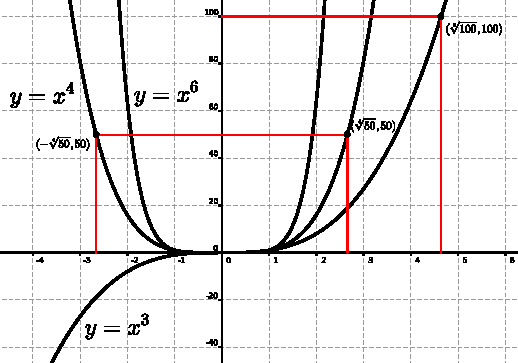
\includegraphics[width=12cm]{pictures/xpot346.pdf}
\end{center}
\end{esimerkki}


\begin{esimerkki}
Suursijoittaja Nalle Mursulla on $5~000$ euroa ylimääräistä rahaa, jonka hän aikoo sijoittaa $30$ vuodeksi.  Nalle Mursu haluaa sijoittamansa pääoman kasvavan $100~000$ euroksi $30$ vuodessa.  Kuinka suuren vuotuisen korkokannan Nalle Mursu tarvitsee sijoitukselleen? 

\emph{Ratkaisu}:  Olkoon vuotuinen korkokanta $r$. \emph{Korkoa korolle -periaatteen} nojalla $5~000$ euron sijoitus kasvaa $30$ vuodessa summaksi $5~000\cdot(1+r)^{30}$.  Merkitsemällä $x=1+r$ saamme yhtälön $5~000\cdot x^{30} = 100~000$.  Jakamalla yhtälö puolittain luvulla $5~000$ päädymme 
potenssiyhtälöön 
$$
x^{30} = 20~000,
$$ 
jonka ratkaisuksi saadaan $x=20~000^{\frac{1}{30}} = 1{,}39\ldots$. Näin
ollen suursijoittaja Nalle Mursun vaatima korkokanta sijoitukselleen on noin $r=1-x=1-1,39=0,39=39~\%$.
\end{esimerkki}

%Potenssifunktiot ovat tapa katsoa potenssiyhtälöitä.

%\laatikko{\emph{Potenssifunktio} on funktio, jossa muuttuja $x$ korotetaan %potenssiin $n$. Potenssifunktion lauseke siis on
%$$
%f(x) = x^n.
%$$
%}

%Potenssiyhtälöä $x^n=a$ voidaan nyt tarkastella tarkastelemalla funktiota %$f(x)=x^n$ ja sen kuvaajaa $y=f(x)$. Tällöin siis $y=a$, eli $y$-akseli vastaa %$a$:n arvoja.

%\missingfigure{Funktioiden $f(x)={x}^3$ ja $g(x)=x^4$ kuvaajat.}

%\laatikko{
%\begin{itemize}
%\item
%Olkoon $n$ \emph{pariton}. Tällöin potenssifunktio $f(x)=x^n$ on kaikkialla %aidosti kasvava ja jatkuva. Tästä seuraa, että yhtälöllä $y=f(x)$ on aina tasan %yksi ratkaisu kaikilla $y$.    
%\item
%Olkoon $n$ \emph{parillinen}. Tällöin potenssifunktio $f(x)=x^n$ on positiivinen, %symmetrinen, jatkuva ja aidosti kasvava, kun $x$ on positiivinen.  %Positiivisuudesta seuraa, että yhtälöllä $y=f(x)$ ei ole ratkaisuja, jos $y$ on %negatiivinen. Symmetriasta $f(x)=f(-x)$ seuraa, että jos $x$ on ratkaisu, niin %myös $-x$ on ratkaisu.  
%\end{itemize}
%}

Yhtälöt, jotka ovat muotoa $a\cdot x^n = b$ (joskus myös muotoa ($a\cdot x^n - b = 0$), ratkaistavuus riippuu useammasta seikasta. Mikäli $n$ on pariton, yhtälö on aina ratkaistavissa (eli sillä on reaalinen juuri):
\begin{align*}
a\cdot x^n &= b \\
x^n &= \frac{b}{a} \\
x &= \sqrt[n]{\frac{b}{a}}
\end{align*}

\begin{esimerkki}
$2x^3 + 16 = 0 \Leftrightarrow 2x^3 = -16 \Leftrightarrow x^3 = -8  \Leftrightarrow x = \sqrt[3]{-8} = -2 $
\end{esimerkki}

Mikäli $n$ on parillinen, yhtälö on ratkaistavissa jos ja vain jos $\frac{b}{a} \geq 0 $. Parillisella potenssifunktiolla voi olla yksi, kaksi tai ei yhtään ratkaisua.

\begin{esimerkki}
$x^2 = 0 \Leftrightarrow x = 0 \\
\Rightarrow$ Yhtälöllä on yksi ratkaisu.
\end{esimerkki}

\begin{esimerkki}
$x^2 - 9 = 0 \Leftrightarrow x^2 = 9 \Leftrightarrow x = \pm 3 \\
\Rightarrow$ Yhtälöllä on kaksi ratkaisua, sillä $3^2 = 9$ ja $(-3)^2 = 9$.
\end{esimerkki}

\begin{esimerkki}
$x^2 + 9 = 0 \Leftrightarrow x^2 = -9 \Leftrightarrow x = \sqrt{-9} \\
\Rightarrow$ Yhtälöllä ei ole reaalista ratkaisua.
\end{esimerkki}

\begin{tehtavasivu}

\begin{tehtava}
Ratkaise: \\
a) $ x^2 = 4 $ \qquad
b) $ x^3 = 27 $ \qquad
c) $ x^5 = -1 $ \qquad
d) $ x^2 - 3 = 0 $ \qquad
e) $ x^3 + 125 = 0 $
\begin{vastaus}
a) $ x = 2 $ \qquad
b) $ x = 3 $ \qquad
c) $ x = -1 $ \qquad
d) $ x = \sqrt{3} $ \qquad
e) $ x = -5 $ 
\end{vastaus}
\end{tehtava}

\begin{tehtava}
Ratkaise \\
a) $ 5x^2 = 25 $ \qquad
b) $ (2x)^3 = 8 $ \qquad
c) $ x^4 = \frac{1}{4} $ \qquad
d) $ (3x)^2 = 36 $ \qquad
e) $ (4x)^2 + 16 = 0 $.
\begin{vastaus}
a) $ x = \sqrt{5} $ \qquad
b) $ x = 1 $ \qquad
c) $ x = \pm\frac{1}{\sqrt{2}} $ \qquad
d) $ x = 2 $ \qquad
e) Ei ratkaisua. 
\end{vastaus}
\end{tehtava}

\begin{tehtava}
Ratkaise potenssiyhtälöt
\begin{alakohdat}
\alakohta{$x^3 = 81$}
\alakohta{$x^5 = 10$}
\alakohta{$x^2 = 4$}
\alakohta{$x^4 = 1$.}
\end{alakohdat}
\end{tehtava}

\begin{tehtava}
Ratkaise potenssiyhtälöt
\begin{alakohdat}
\alakohta{$x^4 - 8 = 0$}
\alakohta{$2x^3 + 7 = 0$}
\alakohta{$\frac{x^2}{4} - \frac{5}{2} = 1$}
\alakohta{$1,51 x^4 - 1,2 = 7,5$.}
\end{alakohdat}
\end{tehtava}

\begin{tehtava}
Muinainen hallitsija Tauno Alpakka rakennuttaa itselleen kuution muotoista palatsia.  Palatsin tilavuuden tulee olla $5~000~\mathrm{m}^3$. 
\begin{alakohdat}
\alakohta{Kuinka korkea palatsista tulee?}
\alakohta{Palatsi päällystetään $10~\mathrm{cm}$:n paksuisella kultakerroksella.  Kuinka monta kiloa kultaa tarvitaan? (Kullan tiheys on $19,23 \cdot 10^3~\mathrm{ kg}/\mathrm{m}^3$.) }
\end{alakohdat}
\end{tehtava}

\end{tehtavasivu}


\chapter{Funktiot}
    \section{Funktio}

Usein ollaan kiinnostuneita siitä, millainen yhteys kahden asian välillä
on. Funktio on matemaattinen työkalu näiden yhteyksien tarkastelemiseen.

\laatikko{
\emph{Funktio} $f$ liittää \emph{muuttujaan} $x$ arvon $f(x)$.

Funktiolla on \emph{määrittelyjoukko} $A$, johon muuttuja $x$ kuuluu, ja \emph{maalijoukko} $B$, johon funktion arvot kuuluvat.
}
%FIXME \todo{Pitäisiköhän tätä funktion määritelmää vielä hioa? Pitäisikö mainita ''Funktio on sääntö''?}
% FIXME Yllä olevasta oli jo pitkä keskustelu, issue 20.

\begin{esimerkki}
Hyödykkeen ja siitä maksettavan arvonlisäveron välistä yhteyttä
voidaan kuvata funktiolla. Valitaan funktion määrittelyjoukoksi
tiettyjen hyödykkeiden joukko,
\[
A = \{\text{ahvenfilee}, \text{AIV-rehu}, \text{auto}, \text{runokirja}, \text{ravintola-ateria}, \text{särkylääke}, \text{televisio}\},
\]
ja arvojoukoksi reaaliluvut. Funktio voi liittää kuhunkin hyödykkeeseen
esimerkiksi siitä maksettavan arvonlisäveroprosentin:
$f(\text{särkylääke}) = 9$ ja $f(\text{televisio}) = 23$.

\begin{center}
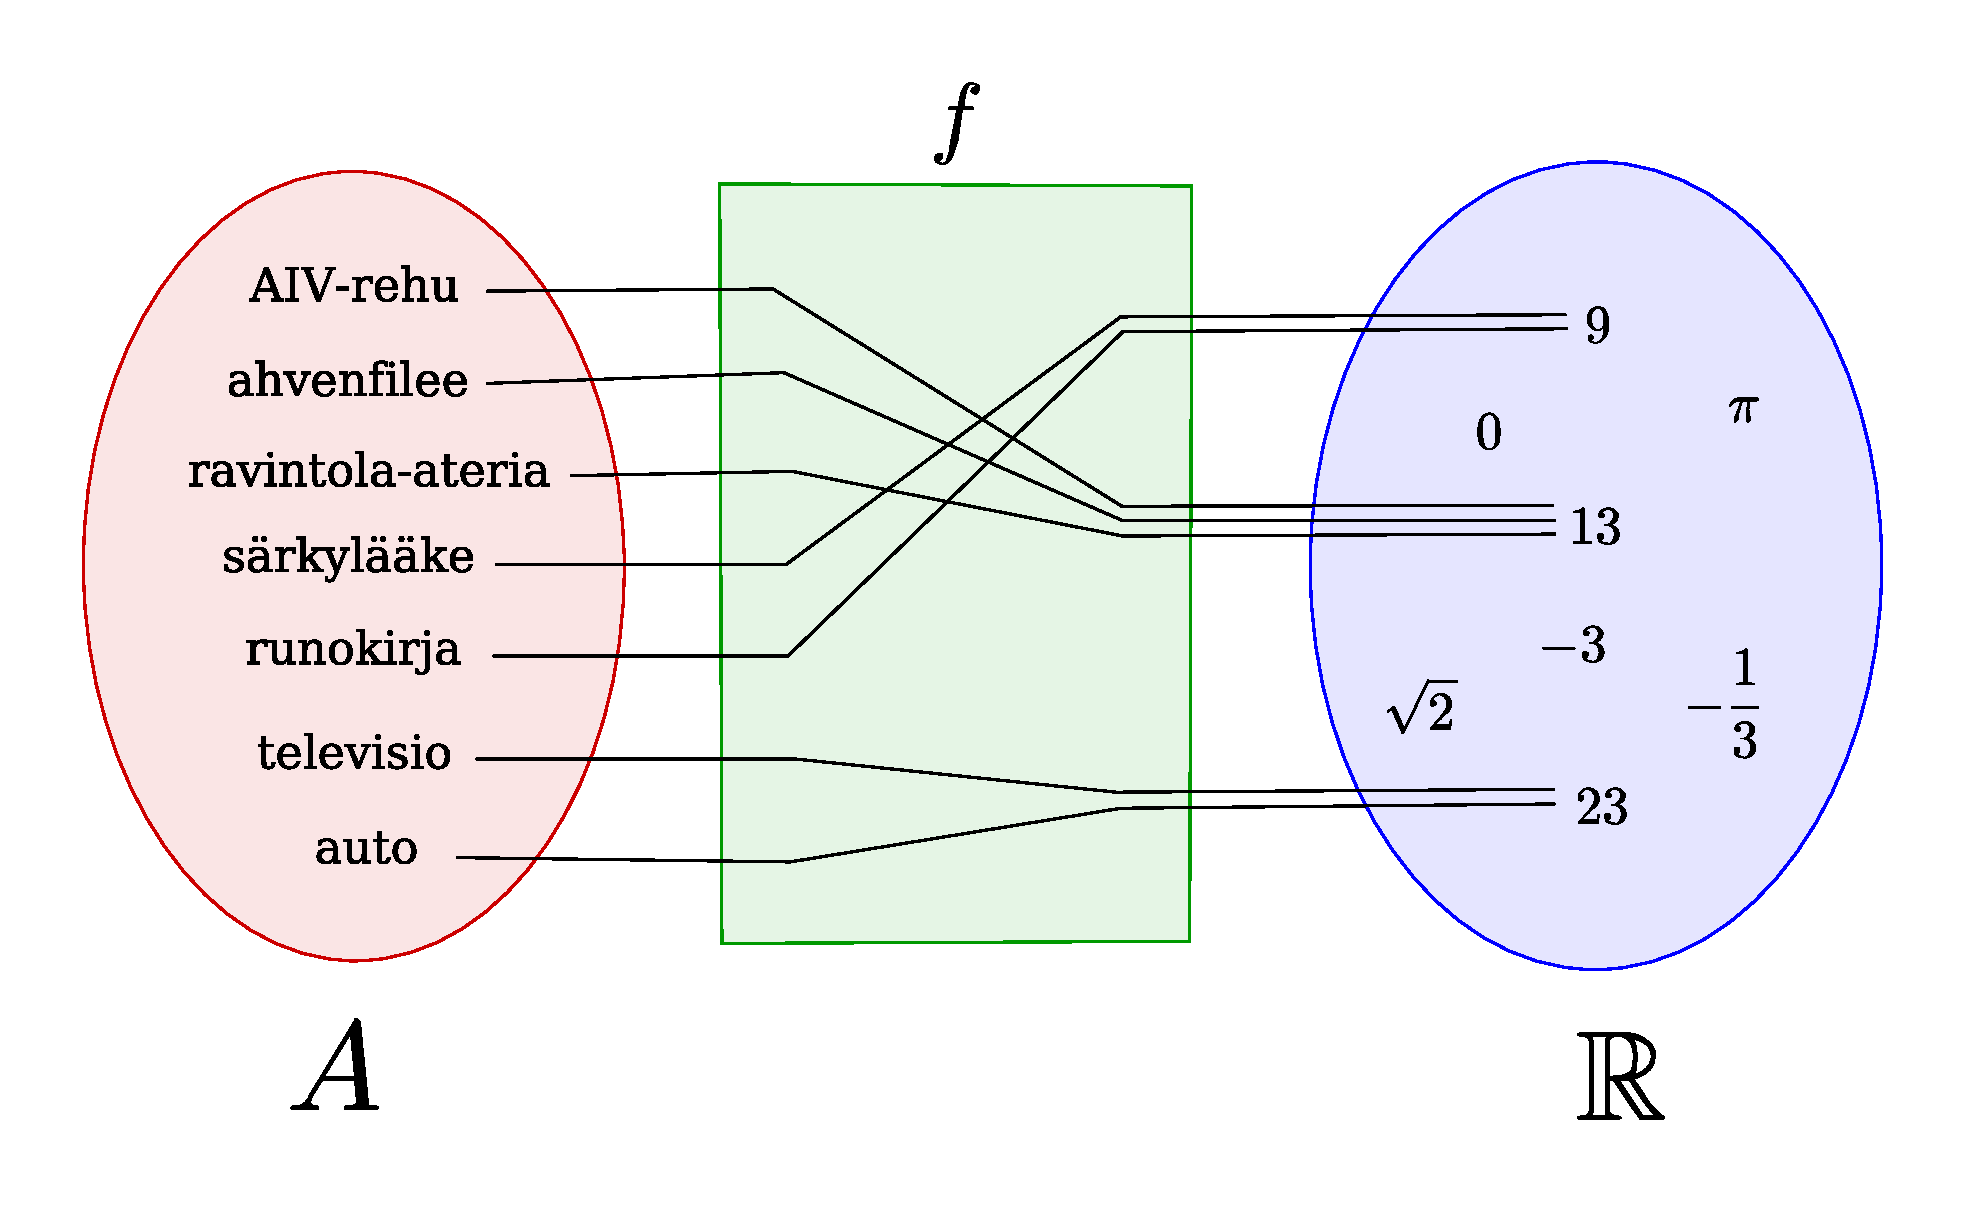
\includegraphics[width=13cm]{pictures/funktiokone.pdf}
\end{center}
\end{esimerkki}

Funktioiden käyttämiseen liittyy joitakin vakiintuneita tapoja:
\begin{itemize}
\item $f(x) = y$ lausutaan: ''Funktio saa arvon $y$ pisteessä $x$'',
\item Funktion määrittely- ja arvojoukko jätetään usein merkitsemättä, jos ne voidaan päätellä asiayhteydestä. Tällä kurssilla arvojoukkona on yleensä reaaliluvut.
\item Toisinaan funktiolle ja funktion kuvaajalle ei tehdä selkeää eroa:
$y = f(x)$ samaistetaan koordinaatistoon piirretyn funktion kuvaajan kanssa.
Periaatteessa funktio ja sen kuvaaja ovat kuitenkin eri asioita.
\end{itemize}

Funktiolla on usein jokin selkeä sääntö, joka voidaan kirjoittaa
matemaattisena lausekkeena.

\begin{esimerkki}
Jos neliön sivun pituutta merkitään muuttujalla $x$, voidaan sivun pituuden
ja neliön pinta-alan välistä yhteyttä kuvata funktiolla
$A(x) = x^2$.
\end{esimerkki}

Funktion määrittelyjoukko koostuu niistä muuttujan arvoista, joilla
funktio on määritelty eli joilla funktion arvo voidaan laskea.

\begin{esimerkki}
Määritellään funktio $f$ lausekkeella
\[
f(x) = \frac{1}{x-1}.
\]
Mikä on funktion määrittelyjoukko?

\textbf{Ratkaisu.}
Funktio $f(x)$ on määritelty, kun nimittäjä $x-1$ on erisuuri
kuin 0. Tämä toteutuu kaikilla $x$:n arvoilla lukuun ottamatta
arvoa $x = 1$. Funktion määrittelyjoukkoon kuuluvat siis
kaikki reaaliluvut paitsi luku $1$.
\end{esimerkki}

Funktion \emph{arvojoukko} sisältää ne maalijoukon alkiot,
jotka funktio saa arvokseen ainakin yhdessä pisteessä.

\begin{esimerkki}
Mikä on edellä määritellyn funktion $f(x)$ arvojoukko?

\textbf{Ratkaisu.}
Arvojoukon selvittämiseksi tutkitaan, millä luvun $a$ arvoilla
yhtälöllä $f(x) = a$ on ratkaisu,
\begin{align*}
a &= \frac{1}{x-1} & &| \, \text{Oletetaan, että $x \neq 1$, jolloin voimme kertoa lausekkeella $(x-1)$ puolittain.} \\
a(x-1) &= 1 \\
x-1 &= \frac{1}{a} \\
x &= 1+\frac{1}{a} & &| \, \text{Havaitaan, että yhtälöllä on ratkaisu
kaikilla $a \neq 0$.}
\end{align*}
Funktion arvojoukkona on siis koko reaalilukujen joukko poislukien luku $0$.
\end{esimerkki}


\subsection*{Tehtäviä}
\begin{tehtava}
Olkoon $f(x)=\frac{2^x+4}{x}$. Laske
\begin{enumerate}[a)]
\item $f(1)$
\item $f(2)$
\item $f(\frac{1}{2})$
\item $f(\frac{1}{3})$
\item $f(0)$
\item $f(-1)$
\end{enumerate}
\begin{vastaus}
\begin{enumerate}[a)]
\item $6$
\item $4$
\item $2\sqrt{2}+8$
\item $3\sqrt[3]{2}+12$
\item ei määritelty
\item $\frac{-9}{2}$
\end{enumerate}
\end{vastaus}
\end{tehtava}

% kai vaikeahko
\begin{tehtava}
Millä $x$:n arvoilla yhtälö $f(f(x)) = x$ pätee, kun
\begin{enumerate}[a)]
\item $f(x) = 1$
\item $f(x) = x$
\item $f(x) = x+1$
\item $f(x) = 2x$
\item $f(x) = 2x+1$?
\end{enumerate}

\begin{vastaus}
\begin{enumerate}[a)]
\item $x = 1$
\item kaikilla $x\in\mathbb{R}$
\item ei ratkaisuja
\item $x = 0$
\item $x = -1$
\end{enumerate}
\end{vastaus}
\end{tehtava}

    \section{Koordinaatisto ja funktion kuvaaja}
Funktioita reaaliluvuilta reaaliluvuille voidaan havainnollistaa koordinaatistossa kuvaajien avulla. Funktion $f$ kuvaajassa koordinaatistoon piirretään ne pisteet, joilla y-koordinaatti on $f$:n arvo sen x-koordinaatissa. Siis kaikilla $f$:n määrittelyjoukon luvuilla $x$ lasketaan $y = f(x)$ ja piirretään piste $(x, y)$ koordinaatistoon. Funktioita voi piirtää helposti myös graafisilla laskimilla tai tietokoneohjelmilla (esimerkiksi Wolfram Alphalla\footnote{\url{http://www.wolframalpha.com/}}).

% Tarvitaan kuvien ja taulukkojen vierekkäin laittamiseen.
\def\vcent#1{\mathsurround0pt$\vcenter{\hbox{#1}}$}

\begin{esimerkki}
Funktion $f(x) = \frac{x}{2} - 1$ kuvaaja sisältää kaikki pisteet $(x, y)$, joilla pätee $y = \frac{x}{2} - 1$:
\begin{center}
\begin{tabular}{cc}
\begin{tabular}{|r|l|}
\hline
$x$ & $y = f(x)$ \\
\hline
$-3$ & $-2,5$ \\
$-2$ & $-2$ \\
$-1$ & $-1,5$ \\
$0$ & $-1$ \\
$1$ & $-0,5$ \\
$2$ & $0$ \\
$3$ & $0,5$ \\
\hline
\end{tabular} &
\vcent{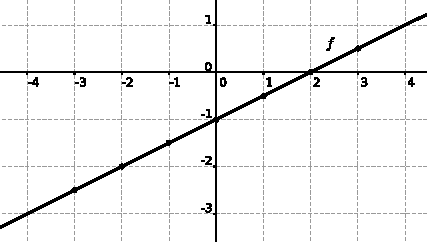
\includegraphics[width=8cm]{pictures/suoraesim.pdf}}
\end{tabular}
\end{center}
\end{esimerkki}

\begin{esimerkki}
Funktion $f(x) = x^2$ kuvaaja sisältää kaikki pisteet $(x, y)$, joilla pätee $y = x^2$:
\begin{center}
\begin{tabular}{cc}
\begin{tabular}{|r|l|}
\hline
$x$ & $y = f(x)$ \\
\hline
$-2$ & $4$ \\
$-1$ & $1$ \\
$-0,5$ & $0.25$ \\
$0$ & $0$ \\
$0,5$ & $0.25$ \\
$1$ & $1$ \\
$2$ & $4$ \\
\hline
\end{tabular} &
\vcent{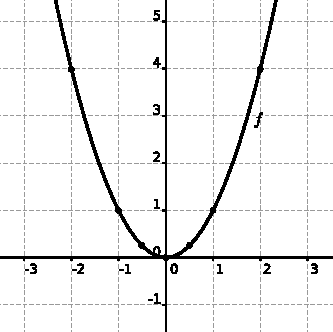
\includegraphics[width=6cm]{pictures/paraabeli.pdf}}
\end{tabular}
\end{center}
\end{esimerkki}

\begin{esimerkki}
Funktion $f(x) = x^3-5x+2$ kuvaaja sisältää kaikki pisteet $(x, y)$, joilla pätee $y = x^3-5x+2$:
\begin{center}
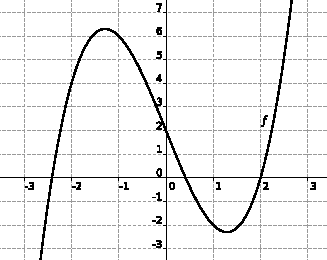
\includegraphics[width=7cm]{pictures/deg3polynomiesim.pdf}
\end{center}
\end{esimerkki}

\begin{tehtavasivu}

\paragraph*{Opi perusteet}

\begin{tehtava}
Hahmottele funktion kuvaaja kynällä ja paperilla tai laskimen avulla. Voit myös käyttää tietokonetta.
\begin{alakohdat}
\alakohta{$f(x) = 2$}
\alakohta{$f(x) = 3x+2$}
\alakohta{$f(x) = x^2$}
\alakohta{$f(x) = \frac{2}{x}$}
\end{alakohdat}

%\begin{vastaus}
%\end{vastaus}
\end{tehtava}

\begin{tehtava}
Laske taulukkoon funktion arvo pisteissä $x=-2$, $x=-1$, $x=0$, $x=1$ ja $x=2$. Hahmottele näiden tietojen avulla funktion kuvaaja.
\begin{alakohdat}
\alakohta{$f(x)= x^2+x+1$}
\alakohta{$f(x)= 3x^2$}
\alakohta{$f(x)= x^3 +2x+2$}
\end{alakohdat}
\begin{vastaus}
\begin{alakohdat}
\alakohta{$f(-2)=3,f(-1)=1, f(0)=1, f(1)=3$ ja $f(2)=7$}
\alakohta{$f(-2)=12, f(-1)=3, f(0)=0, f(1)$ ja $f(2)=12$}
\alakohta{$f(-2)=6, f(-1)=1, f(0)=2, f(1)=5$ ja $f(2)=14$}
\end{alakohdat}
\end{vastaus}
\end{tehtava}

\end{tehtavasivu}

    \chapter{Potenssifunktio}

Kahden muuttujan välinen riippuvuus ei monesti ole suoraan
tai kääntäen verrannollista. Potenssifunktion käyttäminen on eräs
keino kuvata tällaisia riippuvuuksia.

\laatikko{Potenssifunktioita ovat muotoa
$ f(x) = a x^n $ olevat funktiot, jossa $a \neq 0$. }

Eksponenttia $n$ kutsutaan potenssifunktion \emph{asteluvuksi}
tai \emph{asteeksi}.
Potenssifunktion eksponentti voi olla mikä tahansa reaaliluku, mutta
rajoitumme ensin käsittelemään tapauksia, jossa $n = 1, 2, 3\ldots $.

\begin{esimerkki}
Jos neliön sivun pituus on $x$, neliön pinta-ala voidaan laskea
funktiolla $A(x)=x^2$.
Esimerkiksi jos $x = 3$ cm, saadaan neliön pinta-alaksi $A(x) = 9$ cm$^2$.
Vastaavasti kuutiolle: jos $x$ kuvaa kuution särmän pituutta, funktiolla
$V(x)=x^3$ voidaan laskea kuution tilavuus. Sekä $A(x)$ että $V(x)$ ovat
esimerkkejä potenssifunktioista.
\end{esimerkki}

Potenssifunktion aste vaikuttaa funktion kuvaajan muotoon:
\begin{itemize}
  \item
Jos aste on parillinen, kuvaaja on U-kirjaimen muotoinen ja funktio
saa $a$:n merkistä riippuen joko pelkästään positiivisia tai pelkästään
negatiivisia arvoja.
  \item
Jos aste on pariton, kuvaaja muodostaa ''kaksoismutkan'' ja potenssifunktio
saa sekä positiivisia että negatiivisia arvoja.
\end{itemize}

%\missingfigure{Potenssifunktioiden kuvaajat -- yksi parillisilla potensseilla ja toinen parittomilla (kerroin a positiivinen).}
\begin{center}
\begin{kuvaajapohja}{0.5}{-6}{6}{-6}{6}
\kuvaaja{0.2*x**2}{$\frac{1}{5}x^2$}{red}
\kuvaaja{0.2*x**3}{$\frac{1}{5}x^3$}{blue}
\end{kuvaajapohja}
\end{center}
Potenssifunktion tärkeitä erikoistapauksia ovat asteluvut $n = 1$ ja $n = -1$.
Kun $n = 1$, saadaan edellisessä luvussa esitelty suoraan verrannollinen
riippuvuus $x$:n ja $f(x)$:n välillä, ja kun $n = -1$, muuttuja $x$ ja
funktion arvo $f(x)$ ovat kääntäen verrannolliset.

Potenssifunktiota voidaan laajentaa sallimalla eksponentille $n$
myös negatiiviset arvot.
Tällöin funktion muoto muuttuu merkittävästi. Funktio ei myöskään ole
enää määritelty kohdassa $x = 0$, vaan funktion arvot
''räjähtävät äärettömyyteen'', kun y-akselia lähestytään:

%\missingfigure{Potenssifunktioiden kuvaajat - yksi potenssilla -1 ja toinen potenssilla -2.}

\begin{center}
\begin{kuvaajapohja}{0.5}{-6}{6}{-6}{6}
%\kuvaaja{x**(-1)}{$\frac{1}{5}x^2$}{red}
%\kuvaaja{x**(-2)}{$\frac{1}{5}x^3$}{blue}
% FIXME: alla oleva puukotus, että saa äärettömyyteen menevät käppyrät piirtymään oikein
\newcommand{\kuvaajaneg}[3]{
\draw[smooth,color=#3,thick,domain=\kuvaajaminx:-0.01,scale=\kuvaajascale,samples=300] plot function{(#1) < \kuvaajamaxy ? ((#1) > \kuvaajaminy ? (#1) : NaN) : NaN} node[right] {#2};
}
\newcommand{\kuvaajapos}[3]{
\draw[smooth,color=#3,thick,domain=0.01:\kuvaajamaxx,scale=\kuvaajascale,samples=300] plot function{(#1) < \kuvaajamaxy ? ((#1) > \kuvaajaminy ? (#1) : NaN) : NaN} node[right] {#2};
}
\kuvaajaneg{x**(-1)}{$x^{-1}$}{red}
\kuvaajaneg{x**(-2)}{}{blue}

\kuvaajapos{x**(-1)}{}{red}
\kuvaajapos{x**(-2)}{$x^{-2}$}{blue}

\end{kuvaajapohja}
\end{center}

%Potenssifunktiota käsitellään samalla lailla riippumatta eksponentin
%etumerkistä. Huomaa kuitenkin, että $\frac{1}{x^n} \neq 0 $ kaikilla $x$:n %arvoilla.

%Tästä alaspäin on potenssiyhtälöitä, jotka varmaan menee jo päälle
%aiemmin käydyn asian kanssa. Sekaannus meikäläisen osalta... -Matti

\section*{Tehtäviä}

\subsubsection*{Opi perusteet}

\begin{tehtava}
Mikä on seuraavien potenssifunktioiden aste?
\begin{enumerate}[a)]
\item $f(x) = x$
\item $f(x) = 5x^5$
\item $f(x) = \frac{1}{2x}$
\item $f(x) = x^{-2}$
\end{enumerate}
\begin{vastaus}
\begin{enumerate}
\item $1$
\item $5$
\item $-1$
\item $-2$
\end{enumerate}
\end{vastaus}
\end{tehtava}

\begin{tehtava}
Olkoon $f(x)=x^{-3}$. Laske
\begin{enumerate}[a)]
\item $f(1)$
\item $f(2)$
\item $f(-\frac{1}{3})$
\end{enumerate}
\begin{vastaus}
\begin{enumerate}
\item $1$
\item $\frac{1}{8}$
\item $-27$
\end{enumerate}
\end{vastaus}
\end{tehtava}

\subsubsection*{Hallitse kokonaisuus}

\begin{tehtava}
Olkoon $f(x)=x^2$. Millä $x$:n arvoilla
\begin{enumerate}[a)]
\item $f(x)=4$
\item $f(x)=25$
\item $f(x)=121$
\end{enumerate}
\begin{vastaus}
\begin{enumerate}
\item $2$
\item $5$
\item $11$
\end{enumerate}
\end{vastaus}

\end{tehtava}
\begin{tehtava}
Minkä kahden kokonaisluvun välissä yhtälön $x^2 = 12$ ratkaisu on?
\begin{vastaus}
Ratkaisu on lukujen $3$ ja $4$ välissä.
\end{vastaus}
\end{tehtava}

\subsubsection*{Sekalaisia tehtäviä}

\begin{tehtava}
Kuution tilavuus särmän pituuden funktiona on $f(x) = x^3$. Jos kuution tilavuus on $64$, mikä on särmän pituus?
\begin{vastaus}
Särmän pituus on $4$.
\end{vastaus}
\end{tehtava}

    \section{Eksponenttifunktio}

Potenssifunktiossa $f(x) = x^n$ muuttuja $x$ on kantalukuna. Jos muuttuja
$x$ on sen sijaan eksponenttina, saadaan joukko funktioita, joita
kutsutaan \emph{eksponenttifunktioiksi}.

\laatikko{Eksponenttifunktiot ovat muotoa $f(x) = a^x$, $a > 0$,
$a \neq 1$ olevia funktioita.}

Eksponenttifunktioita on kahta tyyppiä: kasvavia ja väheneviä.
Kasvavilla eksponenttifunktioilla $a>1$, esimerkiksi

\begin{center}
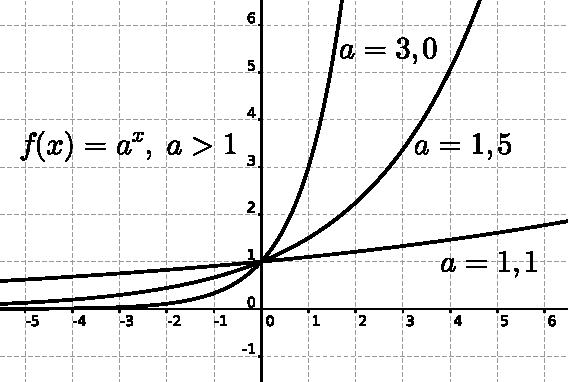
\includegraphics{pictures/apotenssiinxaisompikuinyksi.pdf}
\end{center}

Vähenevillä eksponenttifunktioilla $0<a<1$, esimerkiksi

\begin{center}
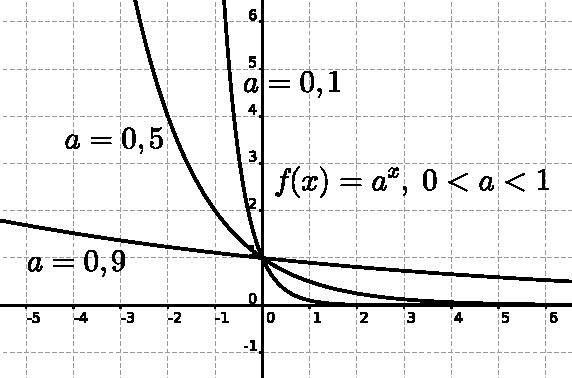
\includegraphics{pictures/apotenssiinxaisompikuinnolla.pdf}
\end{center}

Negatiiviselle kantaluvulle ei ole määritelty yleistä reaalilukupotenssia, 
joten eksponenttifunktiota ei ole määritelty, kun $a < 0$. 

Kun $a=0$ tai $a=1$, eksponenttifunktio pelkistyy vakiofunktioksi.
Lisäksi $0^0$:a ei ole määritelty, joten vaaditaan, että
eksponenttifunktion kantaluvulle $a$ pätee $a>0$ ja $a \neq 1$.

%\emph{Eksponenttiyhtälö} muodostuu, kun kysytään, millä $x$:n arvoilla %eksponenttifunktio saavuttaa tietyn arvon.

\begin{esimerkki}
Millä muuttujan $x$ arvoilla eksponenttifunktio $f(x) = 2^x$ saa arvon
$f(x) = 64$?

\textbf{Ratkaisu.}
Kirjoitetaan tehtävä yhtälöksi: $2^x = 64$. Kokeilemalla huomataan,
että $x = 6$ ratkaisee yhtälön.

Varmistutaan vielä siitä, että yhtälöllä ei ole muita ratkaisuja.
Eksponenttifunktion kantalukuna on $2$, joten eksponenttifunktio on
kasvava. Funktio $f(x) = 2^x$ ei siis voi saada uudelleen arvoa $64$,
kun $x > 6$. Samasta syystä $f(x)$ ei voi olla $64$, kun $x < 6$.

Ainoa ratkaisu yhtälölle on siis $x = 6$.
\end{esimerkki}

\begin{esimerkki}
Millä muuttujan $x$ arvoilla eksponenttifunktio
$f(x) = \left( \frac{1}{2} \right)^{x}$ saa arvon
$f(x) = 1/5$?

\textbf{Ratkaisu.}
Edellisen esimerkin tavoin kokeillaan $x$:n eri arvoja. Havaitaan,
että kun $x = 2$, funktio saa arvon $f(x) = \frac{1}{4}$, ja
kun $x = 3$, on $f(x) = \frac{1}{8}$. Ratkaisu on siis välillä
$2 < x < 3$.

Ratkaisun etsimistä voidaan jatkaa kokeilemalla esimerkiksi
arvoa $x = 2,5$. Näin päästään lähemmäksi ratkaisua, mutta
yhtälön ratkaisu on irrationaalinen, joten sen desimaalikehitelmä
on äärettömän pitkä ja jaksoton. Tarkkaa ratkaisua ei siis saada tällä menetelmällä.

Yleisen eksponenttiyhtälön tarkkaan ratkaisemiseen palataan myöhemmillä
matematiikan kursseilla.
\end{esimerkki}


\subsection*{Eksponentiaalinen malli}

Kun eksponenttifunktiota käytetään kuvaamaan jotakin reaalimaailman
ilmiötä, siitä käytetään nimeä \emph{eksponentiaalinen malli}.

Eksponentiaalinen malli on eräs yleisimmin käytetyistä matemaattisista
malleista. Sillä kuvataan sellaista kasvua tai vähenemistä, jossa
kullakin ajanhetkellä funktion hetkellinen muutos on suoraan
verrannollinen funktion sen hetkiseen arvoon. Tämä muotoillaan
täsmällisesti myöhemmillä matematiikan kursseilla.

\begin{esimerkki}
Soluviljelmässä olevien \emph{Escherichia coli} -bakteerien
määrää voidaan kuvata eksponentiaalisella mallilla: ajanhetkellä
$t = 0$ bakteerien lukumäärä on $1$, ja kullakin aika-askeleella
bakteerien lukumäärä tuplaantuu. Malli voidaan kirjoittaa
\[
f(t) = 2^t, t \ge 0,
\]
jossa $f(t)$ on bakteerien lukumäärä ajanhetkellä $t$.

Huomaa, että funktion $f(t)$ arvot voivat
olla myös rationaalisia tai irrationaalisia, vaikka bakteerien
määrä on kokonaisluku. Yleensä tätä ei pidetä ongelmallisena,
vaan funktiota voidaan käsitellä, ikään kuin bakteerien määrä
olisi jatkuvasti kasvava suure.
\end{esimerkki}

\begin{esimerkki}
Radioaktiivisessa hajoamisessa atomiydinten lukumäärää kuvataan
eksponentiaalisella mallilla. Jos ydinten määrä ajanhetkellä
$t = 0$ on $f(t) = k$, malli voidaan kirjoittaa
\[
f(t) = k \cdot \left( \frac{1}{2} \right)^t, t \ge 0,
\]
jossa $f(t)$ on atomiydinten lukumäärä ajanhetkellä $t$. Atomiydinten
lukumäärä siis puolittuu kullakin aika-askeleella.
\end{esimerkki}

\subsection*{Tehtäviä}

\paragraph*{Opi perusteet}

\begin{tehtava}
Olkoon $f(x) = 4^x$. Laske
\begin{enumerate}[a)]
\item $f(0)$
\item $f(3)$
\item $f(\frac{1}{2})$
\end{enumerate}
\begin{vastaus}
\begin{enumerate}[a)]
\item $1$
\item $64$
\item $2$
\end{enumerate}
\end{vastaus}
\end{tehtava}

\begin{tehtava}
Olkoon $f(x) = 10^x$. Millä $x$:n arvoilla
\begin{enumerate}[a)]
\item $f(x) = 1000$
\item $f(x) = \frac{1}{100}$
\item $f(x) = -1$?
\end{enumerate}
\begin{vastaus}
\begin{enumerate}[a)]
\item $3$
\item $6$
\item Ei ratkaisua.
\end{enumerate}
\end{vastaus}
\end{tehtava}

\paragraph*{Hallitse kokonaisuus}
\begin{tehtava}
Minkä kahden peräkkäisen kokonaisluvun välissä yhtälön
$10^x = 500$ ratkaisu on?
\begin{vastaus}
Ratkaisu on lukujen $2$ ja $3$ välissä.
\end{vastaus}
\end{tehtava}


\begin{tehtava}
Olkoon $f(t) = 20 \cdot 2^t$ bakteerien lukumäärä soluviljelmässä
ajanhetkellä $t$. Millä ajanhetkellä bakteerien lukumäärä on tasan 160?
\begin{vastaus}
Ajanhetkellä $t = 3$.
\end{vastaus}
\end{tehtava}

\begin{tehtava}
Miten muokkaisit edellisen tehtävän funktiota, jos bakteerien lukumääräksi
halutaan 5 ajanhetkellä $t = 0$?
\begin{vastaus}
$f(t) = 5 \cdot 2^t$
\end{vastaus}
\end{tehtava}

\begin{tehtava}
Millä ajanhetkellä atomiydinten määrä on alle $1/200$ alkuperäisestä?
\begin{vastaus}
Ajanhetkellä $t = 8$.
\end{vastaus}
\end{tehtava}

\paragraph*{Sekalaisia tehtäviä}

\begin{tehtava}
(YO 1877 4) Vuosikymmenen 1860--70 kuluessa lisääntyi Helsingin väkiluku puolella vuoden 1860 väkiluvulla. Jos väkiluvun lisäys tapahtuisi seuraavinakin vuosikymmeninä samassa suhteessa, paljonko väkeä Helsingissä olisi 1890, kun siellä 1860 oli 21~700 asukasta? 
	\begin{vastaus}
	73~200 (pyöristämättä 73~237,5)
	\end{vastaus}
\end{tehtava}


% % tähän parempi tehtävä atomiytimistä
%\begin{tehtava}
%Millä ajanhetkellä atomiydinten määrä on alle $1/200$ alkuperäisestä?
%\begin{vastaus}
%Ajanhetkellä $t = 8$.
%\end{vastaus}
%\end{tehtava}


\chapter{Kertaustehtäviä}
    \chapter{Harjoituskokeita}

\section*{Harjoituskoe 1}

\begin{description}
	\item[] Ei laskinta.
	\item[1.] Kerro jokin \\
	(a) aina tosi yhtälö \\
	(b) joskus tosi yhtälö (ja milloin se on tosi) \\
	(c) aina epätosi yhtälö.
	\item[2.] Laske \\
	(a) $\sqrt{144}$ \qquad
	(b) $\sqrt{196}$ \qquad
	(c) $\sqrt[3]{64}$ \qquad
	(d) $\sqrt[3]{216}$.
	\item[3.] Muuta murtoluvuksi \\
	(a) $0,45$ \qquad
	(b) $0,33\ldots$ \qquad
	(c) $0,2857142\ldots$ \qquad
	(d) $0,388\ldots$.
	\item[4.] Laske auki \\
	(a) $(a+b)^2$ \qquad
	(b) $(a-b)^2$ \qquad
	(c) $(a+b)(a-b)$.
	\item[5.] Mitkä seuraavista luvuista ovat alkulukuja? \\
	(a) $11$ \qquad
	(b) $4$ \qquad
	(c) $29$ \qquad
	(d) $39$.
	\item[6.] Ratkaise \\
	(a) $x^2 = 1$ \qquad
	(b) $x^4 = x^2$.
	\item[7.] Muuta seuraavat kymmenjärjestelmän luvut heksadesimaaliluvuiksi. \\
	(a) $175$ \qquad
	(b) $384$.
	\item[8.] Funktio $f$ määritellään kaavalla $f(x) = x^2 + 2x + 3$. Ilmaise $f(f(x))$ muodossa, jossa ei ole termiä $f(x)$.
\end{description}

\section*{Harjoituskoe 2}

\begin{description}
	\item[] Ei laskinta.
	\item[1.] Kerro jokin \\
	(a) kokonaisluku, joka ei ole luonnollinen luku \\
	(b) rationaaliluku, joka ei ole kokonaisluku \\
	(c) reaaliluku, joka ei ole rationaaliluku.
	\item[2.] Ratkaise \\
	(a) $11x=77$ \qquad
	(b) $8x+174=50$ \\
	(c) $7x+7=5x$ \qquad
	(d) $6x+7=8x+1$.
	\item[3.] Muuta desimaaliluvuksi \\
	(a) $\frac{3}{10}$ \qquad
	(b) $\frac{3}{16}$ \qquad
	(c) $\frac{5}{9}$ \qquad
	(d) $\frac{5}{11}$.
	\item[4.] Tuoreessa ananaksessa veden osuus on 80\% ananaksen massasta ja A-, B- ja C-vitamiinien yhteenlaskettu osuus 0,05\% massasta. Ananas kuivatetaan niin, että veden osuus laskee 8 prosenttiin ananaksen massasta. Kuinka suuri on A-, B- ja C-vitamiinien osuus kuivatun ananaksen massasta? (Luvut eivät ole faktuaalisia.)
	\item[5.] Muuta seuraavat kymmenjärjestelmän luvut binääriluvuiksi. \\
	(a) $100$ \qquad
	(b) $128$.
	\item[6.] Sievennä \\
	(a) $\frac{a^2 b^2}{a}$, $a \neq 0$ \qquad
	(b) $3(a^2+1)-2(a^2-1)$ \\
	(c) $ab(a+2a)$ \qquad
	(d) $(a^3 b^2 c)^2$.
	\item[7.] Olkoon $f(t) = 35 \cdot 2^t$ bakteerien lukumäärä soluviljelmässä ajanhetkellä $t$ (sekuntia). Monenko sekunnin kuluttua bakteereita on yli 1000? Yhden sekunnin tarkkuus ylöspäin pyöristettynä riittää.
	\item[8.] Määritellään kahdelle järjestetylle lukunelikolle $(a, b, c, d)$ laskutoimitus $\odot$ seuraavasti: $(a_1, b_1, c_1, d_1) \odot (a_2, b_2, c_2, d_2) = (a_1 a_2 + b_1 c_2, a_1 b_2 + b_1 d_2, c_1 a_2 + d_1 c_2, c_1 b_2 + d_1 d_2)$. Laske $(1, 1, 1, 0) \odot (1, 1, 1, 0)$.

\end{description}

    \section{Ylioppilaskoetehtäviä}

Ylioppilaskokeissa on yleensä tehtäviä tai tehtävien alakohtia, joiden ratkaiseminen on mahdollista ensimmäisen kurssin tiedoin.

\begin{description}

    \item[(K2012/1b)]  Ratkaise yhtälö
                        \[\frac{x}{6} - \frac{x-3}{2} - \frac{7}{9} = 0 \]
    \item[(K2012/2a)]  Laske lausekkeen $ \frac{15}{4} - \left( \frac{6}{3} \right)^2 $ arvo.
    \item[(S2011/1b)]  Ratkaise yhtälö
                        \[ \frac{4x - 1}{5} = \frac{x + 1}{2} + \frac{3 - x}{4}. \]
%    \item[(S2011/2a)]  Sievennä välivaiheet esittäen lauseke
%                       \[ \frac{1}{\sqrt{2} + \frac{1}{2 + \sqrt{2}}} \]
    \item[(K2011/1a)]  Ratkaise yhtälö
                        \[ \frac{2}{x} = \frac{3}{x - 2} \]
    \item[(K2011/2a)]  Osakkeen arvo oli 35,50 euroa. Se nousi ensin 12~\%,
                        mutta laski seuraavana päivänä 10~\%. Kuinka monta prosenttia
                        arvo nousi yhteensä näiden muutosten jälkeen?
    \item[(S2010/1a)]  Sievennä lauseke $ (a + b)^2 - (a - b)^2 $.
    \item[(K2010/1b)]  Sievennä lauseke $ (\sqrt{a} + 1)^2 - a - 1 $.
    \item[(S2009/1c)]  Osoita, että $ \sqrt{27 - 10 \sqrt{ 2} } = 5 - \sqrt{2} $.
    \item[(S2009/2b)]  Ratkaise yhtälö $ \sqrt{x + 2 } = 3  $.
    \item[(K2009/1a)]  Sievennä $ \frac{a^2}{3} - \left( \frac{-a}{3} \right)^2 $.
    \item[(S2008/1b)]  Sievennä lauseke
                        \[ \frac{1}{x} - \frac{1}{x^2} + \frac{1 + x}{x^2} \]
    \item[(S2009/2b)]  Ratkaise yhtälö
                        \[ \frac{x}{6} - \frac{x - 2}{3} = \frac{5}{12} \]
    \item[(K2008/4)]   Vuonna 2007 alennettiin parturimaksujen arvonlisäveroa 22
                        prosentista 8 prosenttiin. Jos alennus olisi siirtynyt
                        täysimääräisenä parturimaksuihin, kuinka monta prosenttia
                        ne olisivat alentuneet? Arvonlisävero ilmoitetaan prosentteina
                        verottomasta hinnasta ja se on osa tuotteen tai palvelun hintaa.
    \item[(S2007/1c)]  Ratkaise $L$ yhtälöstä
                        \[ t = \frac{1}{2\pi\sqrt{LC}} \]
    \item[(S2007/4)]   Tuotteen hintaa korotettiin $p$ prosenttia, jolloin menekki väheni.
                        Tämän johdosta hinta päätettiin alentaa takaisin alkuperäiseksi.
                        Kuinka monta prosenttia korotetusta hinnasta alennus oli?
    \item[(K2007/1c)]  Sievennä lauseke $ \sqrt[3]{a \sqrt{a}} \quad (a > 0) $.
    \item[(K2007/3a)]  Merivettä, jossa on 4,0 painoprosenttia suolaa, haihdutetaan
                        altaassa, kunnes sen massa on vähentynyt 28~\%. Mikä on
                        suolapitoisuus haihduttamisen jälkeen? Anna vastaus prosentin
                        kymmenesosan tarkkuudella. 
    \item[(K2007/3b)]  Mikä on vuotuinen korkoprosentti, jos tilille talletettu rahamäärä
                        kasvaa korkoa korolle 1,5--kertaiseksi 10 vuodessa? Lähdeveroa
                        ei oteta huomioon. Anna vastaus prosentin sadasosan 
                        tarkkuudella.
        \item[(S2006/5)]   Hopean ja kuparin seoksesta tehty esine painaa 150~g, ja sen
                       tiheys on 10,1~kg/dm\(^3\). Kuinka monta painoprosenttia 
                        esineessä on hopeaa ja kuinka monta kuparia, kun hopean tiheys on 
                        10,5~kg/dm\(^3\) ja kuparin 9,0~kg/dm\(^3\)?
    \item[(K2006/1a)]  Ratkaise $x$ yhtälöstä $4x + 2 =  3 - 2(x + 4)$.
    \item[(K2006/1c)]  Sievennä lauseke 
                        \[ \frac{1}{a - 1} \left( a - \frac{1}{a} \right) \]
     \item[(K2006/4)]   Kesämökin rakentaminen tuli 25~\% arvioitua kalliimmaksi.
 Rakennustarvikkeet olivat 19~\% ja muut kustannukset 28~\% 
                        arvioitua kalliimpia. Mikä oli rakennustarvikkeiden arvioitu osuus ja 
                        mikä lopullinen osuus kokonaiskustannuksista?
    \item[(S2005/1a)]  Ratkaise reaalilukualueella yhtälö 
                        \[ 2(x - 1) + 3(x + 1 ) = -x \]
    \item[(S2005/1c)]  Ratkaise reaalilukualueella yhtälö $ x^{16} = 256 $.
    \item[(K2005/1a)]  Sievennä lauseke
                        \[ \frac{x}{1 - x} + \frac{x}{1 + x} \]
%    \item[(K2005/2a)]  Ratkaise yhtälöryhmä
%                        \[
%                         \left\{
%                         \begin{aligned}
%                              x + y &= a \\
%                              x - y &= 2a
%                         \end{aligned}
%                         \right.
%                      \]
    \item[(K2005/3)]   Asuinrakennuksesta saadut vuokrat ovat 12~\% pienemmät kuin
                        ylläpitokustannukset. Kuinka monta prosenttia vuokria olisi
                        korotettava, jotta ne tulisivat 10~\% suuremmiksi kuin 
                        ylläpitokustannukset, jotka samanaikaisesti kohoavat 4~\%?
    \item[(K2004/3)]   Perheen vuokramenot olivat 25~\% tuloista. Vuokramenot nousivat
                        15~\%. Montako prosenttia vähemmän rahaa riitti muuhun
                        käyttöön korotuksen jälkeen?
    \item[(S2003/5)]   Päärynämehusta ja omenamehusta tehdyn sekamehun sokeripitoisuus
                        on 11~\%. Määritä mehujen sekoitussuhde, kun päärynämehun
                        sokeripitoisuus on 14~\% ja omenamehun 7~\%.

    \item[(K2003/1)]   Sievennä lausekkeet
        \begin{enumerate}[(a)]
            \item $ \sqrt{3\frac{3}{4}} \big/ \sqrt{1\frac{2}{3}} $
            \item $ \left( \frac{x}{y} + \frac{y}{x} -
                    2 \right) \big/ \left( \frac{x}{y} - \frac{y}{x} \right) $.
        \end{enumerate}
    \item[(S2002/2)]   Vuoden 1960 jälkeen on nopeimman junayhteyden matka-aika
                        Helsingin ja Lappeenrannan välillä lyhentynyt 37 prosenttia.
                        Laske, kuinka monta prosenttia keskinopeus on tällöin noussut.
                        Oletetaan, että radan pituus ei ole muuttunut.
    \item[(S2002/4a)]  Olkoon $ a \neq 0$ ja $b \neq 0 $. Sievennä lauseke
                        \[
                            \frac{a + \frac{b^2}{a} } {b + \frac{a^2}{b} }
                        \]
    \item[(K2002/3)]   Vuonna 2001 erään liikeyrityksen ulkomaille suuntautuvan
                        myynnin arvo kasvoi 10~\% vuoteen 2000 verrattuna. Samaan
                        aikaan myynnin arvo kotimaassa väheni 5~\%. Tällöin koko
                        myynnin arvo kasvoi 6~\%. Laske, kuinka monta prosenttia
                        myynnistä meni vuonna 2000 ulkomaille.
    \item[(S2001/1)]   Ratkaise lineaarinen yhtälöryhmä
                       \[
                         \left\{
                          \begin{aligned}
                             3x - 2y &= 1 \\
                             4x + 5y &= 2                      
                         \end{aligned}
                         \right.
                       \]
    \item[(S2001/3)]   Juna lähtee Tampereelta klo 8.06 ja saapuu Helsinkiin klo 9.58.
                        Vastakkaiseen suuntaan kulkeva juna lähtee Helsingistä klo 8.58
                        ja saapuu Tampereelle klo 11.02. Matkan pituus on 187 kilometriä.
                        Oletetaan, että junat kulkevat tasaisella nopeudella, eikä
                        pysähdyksiin kuluvia aikoja oteta huomioon. Laske kummankin
                        junan keskinopeus. Millä etäisyydellä Helsingistä junat
                        kohtaavat, ja paljonko kello tällöin on? 
    \item[(K2001/4)]   Säiliö sisältää 2,3~kg ilmaa, ja pumppu poistaa jokaisella
                        vedolla 5~\% säiliössä olevasta ilmasta. Kuinka monen vedon
                        jälkeen säiliössä on vähemmän kuin 0,2~kg ilmaa?
    \item[(S2000/1)]   Sievennä seuraavat lausekkeet:
                        \begin{enumerate}[(a)]
                            \item $ \left( x^{n - 1} \right)^{n - 1} \cdot
                                \left( x^{n} \right)^{2 - n} $
                            \item $ \sqrt[3]{a} \; ( \sqrt[3]{a^2} - \sqrt[3]{a^5}) $
                        \end{enumerate}
    \item[(S2000/3)]   Matkaa kuljetaan tasaisella nopeudella. Kun matkasta on
                        jäljellä 40~\%, nopeutta lisätään 20~\%. Kuinka monta
                        prosenttia koko matkaan kuluva aika tällöin lyhenee?

\end{description}

    \section{Pääsykoetehtäviä}

\subsection*{Arkkitehtivalinta}

\begin{description}
    \item[(2012/1)] Taloyhtiössä on $210$ asukasta. Taloyhtiö perii vesimaksua
        $15$ \euro/henkilö/kk. Kaupunki perii taloyhtiöltä vesimaksua
        kokonaiskulutuksen mukaan $3,17$~\euro $/ \mathrm{m}^3$.
        Taloyhtiön toteutunut kokonaisvedenkulutus on asukasta kohden
        155 litraa vuorokaudessa, mihin sisältyy hukkaan valuvia
        vuotoja yhtiötä kohden $1500~\mathrm{m}^3$ vuodessa. Oletamme,
        että vuodessa on $365$ vuorokautta.
                    
    \begin{alakohdat}
        \alakohta{Kuinka monta litraa vettä taloyhtiössä valuu hukkaan minuutissa?}
        \alakohta{Vuodot tukitaan. Montako prosenttia vesimaksua voitaisiin laskea tai tulee korottaa, jotta vesimaksu tällöin kattaisi taloyhtiön vuotuiset vesikulut?}
    \end{alakohdat}
    
    Anna vastaukset kolmen numeron tarkkuudella.
\end{description}

% Vastaus: a) 2,85~l/min b) laskea 12,9 prosenttia

\begin{description}
    \item[(2010/3)] Arkkitehdit M. Uoto, F. Örm ja S. Hapé ovat suunnitelleet Aalto-yliopiston aulaan kullatusta teräskuutiosta muodostuvan taideteoksen. Kultaus on ohut.
    
    Toteutuksen aikana teoksen sijoituspaikka muuttuu, jolloin teräskuution tilavuutta kasvatetaan 19~\% alkuperäisestä. Loppulaskutuksessa materiaalikustannusten todetaan kasvaneen samaiset 19~\% alkuperäisestä budjetista.                   
    \begin{alakohdat}
        \alakohta{Paljonko kultaukseen käytetyn kullan määrä kasvoi toteutuksen aikana?}
        \alakohta{Teräksen yksikköhinta ei toteutuksen aikana muuttunut. Miten kullan yksikköhinta siis muuttui?}
    \end{alakohdat}
    
    Anna vastaukset prosentteina $0,1$ prosenttiyksikön tarkkuuteen pyöristettynä.
\end{description}

\subsection*{Diplomi-insinöörivalinta}
\begin{description}
	\item[(2012/3)] Asumistukea maksetaan 80~\% vuokran määrästä, siltä osin kuin
        vuokra ei ylitä 252 euroa. Vuokran määrää vähennettynä asumistuella
        kutsutaan omavastuuksi.
        
		\begin{alakohdat}
			\alakohta{Minkä suuruinen vuokra on, kun omavastuu on puolet vuokrasta?}
		\end{alakohdat}
	
	\item[(2009/1)] Kokonaistuotanto jaetaan materian ja palveluiden tuotantoon.
        Verrataan tuotantoa tammikuussa 2008 tammikuuhun 2009. Tänä vuoden pituisen
        tarkastelujakson aikana materiatuotanto kasvoi 2,0~\% ja palvelutuotanto laski 7,0~\%.
	
	   Kuinka suuri oli materiatuotannon osuus kokonaistuotannosta tammikuussa 2009,
	   
    	\begin{alakohdat}
    		\alakohta{kun tammikuussa 2008 materia- ja palvelutuotanto olivat yhtäsuuret?}
    		\alakohta{kun vertailuaikana kokonaistuotanto laski 2,0~\%?}
    	\end{alakohdat}
    	
	   Anna kummatkin vastaukset 0,1~\%-yksikön tarkkuuteen pyöristettynä.

	\item[(2008/2)] Yritys hankkii 5000~kg raaka-ainetta, josta on vettä 5,40~\%
        (painoprosenttia) ja väripigmenttiä 2,60~\%. Ennen käyttöä raaka-aine on
        laimennettava siten, että lisäyksen jälkeen sekoituksesta 6,60~\% on vettä.
	
    	\begin{alakohdat}
    		\alakohta{Miten paljon hankittuun raaka-aineeseen tulee lisätä vettä, jotta haluttu vesipitoisuus saavutetaan?}
    		\alakohta{Miten paljon vettä ja väripigmenttiä tulee lisätä hankittuun raaka-aineeseen, jotta haluttu vesipitoisuus saavutetaan, ja lisäksi väripigmentin suhteellinen osuus massasta säilyy alkuperäisenä 2,60~\%:na?}
    	\end{alakohdat}
    	
    	Anna vastaukset sadan gramman tarkkuudella.

	\item[(2007/1)] Vaaleissa kaikkiaan 39~300 äänestäjästä 45~\% äänestää varmasti
        puoluetta A ja 47~\% puoluetta B. Loput ovat ns. liikkuvia äänestäjiä,
        jotka eivät ole vielä päättäneet kantaansa.
	
    	\begin{alakohdat}
    		\alakohta{Oletetaan, että kaikki äänioikeutetut äänestävät. Kuinka monta liikkuvien äänestäjien ääntä puolueen A täytyy tällöin kerätä saadakseen enemmistön, vähintään puolet annetuista äänistä?}
    		\alakohta{Oletetaan, että täsmälleen kolmasosa liikkuvista äänestäjistä jättää äänestämättä. Kuinka monta prosenttia liikkuvien äänestäjien annetuista äänistä puolueen A täytyy tällöin kerätä saadakseen enemmistön kaikista annetuista äänistä?}
    	\end{alakohdat}	 	
	
\end{description}

\subsection*{Matematiikan ja tilastotieteen valinta}

\begin{description}
	\item[(2012/1a)] Ratkaise yhtälö $\frac{3}{2}x - \frac{2}{3} = \frac{2}{3}x - \frac{1}{4}$.
	\item[(2011/1)] Oletetaan, että polttoaineessa E05 on etanolia 5~\% ja
        bensiiniä 95~\% ja polttoaineessa E10 etanolia 10~\% ja bensiiniä 90~\%.
        Oletetaan myös, että etanolin energiasisältö on $\frac{2}{3}$ puhtaan bensiinin
		energiasisällöstä. Jos tietyllä autolla 100~km kulutus on 10 litraa
        polttoainetta E05, paljonko kulutus on polttoainetta E10? Anna vastaus
        sievennettynä murto- tai sekalukuna. Jos polttoaineen E10 hinta on 1,60~€/l
        ja polttoaineen E05 hinta on 1,65~€/l, kumpaa on edullisempaa käyttää?
	\item[(2008/1)] Matkailuauton nopeus on 80~km/h, mutta kolmasosalla matkasta
        Jyväskylästä Heinolaan se laskee tietöiden takia 40~kilometriin tunnissa.
        Kuinka paljon tietyöt alentavat matkailuauton keskinopeutta välillä Jyväskylä--Heinola?
\end{description}

\subsection*{Tekniikan ja liikenteen alan AMK-valinta}

\begin{description}
	\item[(K2012/3)] Erään tuotteen valmistuskustannuksista raaka-aineiden osuus on
        65~\% ja palkkojen osuus on 35~\%.
        
    	\begin{alakohdat}
    		\alakohta{Jos työntekijät saavat 5~\% palkankorotuksen, niin kuinka monta prosenttia tuotteen valmistuskustannukset kasvavat?}
    		\alakohta{Jos toisaalta valmistuskustannukset halutaan pitää ennallaan palkankorotuksen jälkeen, niin montako prosenttia raaka-ainekustannusten pitää pienentyä?}
    	\end{alakohdat}	 

	\item[(K2012/4)] Esitä luku $\frac{1}{1+\frac{1}{1+\frac{1}{1+1}}}$ yhtenä murtolukuna (siis muodossa $\frac{m}{n}$ [missä $m$ ja $n$ ovat kokonaislukuja, toim. lis.]).
	\item[(S2011/2)] Olkoon $a=132$ ja  $b=112$. Kuinka monta prosenttia 
		\begin{alakohdat}
			\alakohta{luku a on suurempi kuin luku b}
			\alakohta{luku b on pienempi kuin luku a}
			\alakohta{luku b on luvusta a? }
		\end{alakohdat}
	\item[(K2011/1)] Laske lukujen $\frac{1}{3}$ ja $-\frac{7}{3}$
		\begin{alakohdat}
			\alakohta{summan vastaluku}
			\alakohta{summan käänteisluku }
			\alakohta{käänteislukujen summa.}
		\end{alakohdat}
	\item[(K2011/2)] Yksi kilogramma etanolia tuottaa palaessaan energiaa 26,8~MJ
        ja vastaavasti yksi kilogramma puhdasta bensiiniä tuottaa palaessaan energiaa
        42,6~MJ. Kuinka monta prosenttia enemmän energiaa puhdas bensiini tuottaa
        palaessaan kuin 95~E10 -bensiini, joka sisältää 10~\% etanolia? Ilmoita
        vastaus yhden desimaalin tarkkuudella. 
\end{description}

\subsection*{Kauppatieteiden valintakoe}

Kauppatieteiden valintakokeen tehtävät ovat monivalintoja. Kussakin tehtävässä on täsmälleen yksi oikea vastausvaihtoehto. Kokeessa saa käyttää ainoastaan ns. nelilaskinta, jolla voi laskea vain yhteen-, vähennys-, kerto- ja jakolaskuja sekä neliöjuuren. Seuraavia tehtäviä ratkoessasi sinun kannattaa miettiä, miten toimisit, jos käytössäsi olisi vain nelilaskin.

\begin{description}
	\item[(2002/38)] Mikä on lukujen $a=2^{1/2}$, $b=3^{1/3}$ ja $c=5^{1/5}$ suuruusjärjestys?
        
		\begin{alakohdat}
			\alakohta{$a>b>c$}
			\alakohta{$a>c>b$}
			\alakohta{$b>a>c$}
			\alakohta{$c>a>b$}
		\end{alakohdat}

%Oikea vastausvaihtoehto: c

	\item[(2008/43)] TietoEnatorin liikevaihto vuonna $2007$ oli $1\,772{,}4$ MEUR (miljoona Euroa). Mikä
	alla olevista vaihtoehdoista on lähimpänä vuoden $1999$ liikevaihtoa, kun
	liikevaihdon keskimääräinen vuotuinen muutosprosentti kahdella desimaalilla on
	ollut $3{,}96 \%$? Keskimääräinen muutosprosentti on luku, joka ilmaisee kuinka paljon
	liikevaihto olisi vuosittain prosentuaalisesti kasvanut, jos prosentuaalinen kasvu olisi
	ollut vakio.
        
		\begin{alakohdat}
			\alakohta{$1\,299{,}1$ MEUR}
			\alakohta{$1\,346{,}0$ MEUR}
			\alakohta{$1\,704{,}9$ MEUR}
			\alakohta{$1\,249{,}6$ MEUR}
		\end{alakohdat}

%Oikea vastausvaihtoehto: a

	\item[(2004/40)] Piensijoittajan rahavarat $r$ vuoden alussa ovat 1 000 \euro, ja ne kasvavat korkoa vuotuisen korkotekijän $R=1{,}04$ mukaisesti. Vuoden lopussa korko lisätään pääomaan, ja seuraavana vuotena vuotuinen korkotekijä on $R=1{,}10$. Korkotuotto kahdelta vuodelta on (lähimpään kokonaislukuun pyöristettynä)
        
		\begin{alakohdat}
			\alakohta{$145$ \euro.}
			\alakohta{$140$ \euro.}
			\alakohta{$100$ \euro.}
			\alakohta{$144$ \euro.}
		\end{alakohdat}

%Oikea vastausvaihtoehto: d

	\item[(2003/33)] Yhtä tuotetta valmistavan monopoliyrityksen kuukauden tarjontamäärän ollessa $q$ (yks/kuukausi) on tuotteen hinta $p$ (euroa/yks) annettu hintafunktiolla $p = 100-q$. Kun kyseessä on monopoli, yritys määrää markkinahinnan $p$ valitsemalla tuotantomäärän $q$, jolloin hinta määräytyy hintafunktion mukaisesti. Yrityksen tuotantokustannukset $c(q)$ (euroa/kuukausi) tuotantomäärän $q$ funktiona ovat\\
$c(q)=100+80q$, kun $q\leq 15$, ja\\
$c(q)=700+40q$, kun $q\geq 15$.\\
Yrityksen voitto $pq-c(q)$ saavuttaa maksimiarvonsa, kun
        
		\begin{alakohdat}
			\alakohta{$q=10$.}
			\alakohta{$q=15$.}
			\alakohta{$q=30$.}
			\alakohta{$q=60$.}
		\end{alakohdat}

%Oikea vastausvaihtoehto: c

	\item[(2000/33)] Erään tuotteen kysyntämäärä $d$ (yksikköä) riippuu yksikköhinnasta $p$ (mk/yksikkö) funktion $d=5000p^{-1{,}5}$ mukaisesti. Tuotteen yksikkökustannukset ovat vakio $15$ mk/yksikkö. Suurin nettotuotto saadaan tällöin hinnalla
        
		\begin{alakohdat}
			\alakohta{$40$ mk.}
			\alakohta{$45$ mk.}
			\alakohta{$50$ mk.}
			\alakohta{$55$ mk.}
		\end{alakohdat}

%Oikea vastausvaihtoehto: b
	
\end{description}


\Closesolutionfile{ans}
